\documentclass
[
	paper = a4,
    pagesize,
	12 pt,
	oneside,                       % Chose ›oneside‹ for digital version, ›twoside‹ for printed version.
    open = right,
	DIV = calc,
	BCOR = 0 mm,                   % Binding correction. Only necessary for printed version. Depends on actual binding.
	bibtotoc
]
{scrbook}

% Do not change the following commands.
\newcommand*{\printTitle}{}
\newcommand*{\printAuthor}{}
\newcommand*{\printDateOfBirth}{}
\newcommand*{\printPlaceOfBirth}{}
\newcommand*{\printSubject}{}
\newcommand*{\myTitle}[1]{\renewcommand*{\printTitle}{#1}}
\newcommand*{\myName}[1]{\renewcommand*{\printAuthor}{#1}}
\newcommand*{\myDateOfBirth}[1]{\renewcommand*{\printDateOfBirth}{#1}}
\newcommand*{\myPlaceOfBirth}[1]{\renewcommand*{\printPlaceOfBirth}{#1}}
\newcommand*{\mySubject}[1]{\renewcommand*{\printSubject}{#1}}

\myTitle{High-level Visualization of Graph Algorithms}  % Change!
\myName{Julius Milian Severin}  % Change!
\myDateOfBirth{March~12, 1995}  % Change!
\myPlaceOfBirth{Berlin, Germany}  % Change!
\mySubject{{Graph Algorithms}{Visualization}}  % Change!

\usepackage[utf8]{inputenc}
\usepackage[T1]{fontenc}
\usepackage[english]{babel}

\usepackage{graphicx}

\graphicspath{{Images/}}

\usepackage{pgf}

\usepackage							% Microtypography tuning.
[
	protrusion = true,
	expansion = false,
	tracking = true,
	kerning = true,
	spacing = false,
	babel = true
]
{microtype}							% http://ctan.mirrorcatalogs.com/macros/latex/contrib/microtype/microtype.pdf

\SetTracking[unit = space]{font = */*/*/sc/*}{25}   % Adjust kerning for small caps.

\SetExtraKerning[unit = space]		% Adjusted kerning for certain characters.
{
	font = */*/*/*/*
}
{
	: = {100, },
	; = {100, },
	? = {150, 150},
	! = {150, 150},
	: = {250, },
	; = {150, },
	? = {250, 250},
	! = {250, 250},
	» = { , -200},
	« = {-200, },
	› = { , -200},
	‹ = {-200, },
	– = {200, 250},
	— = {200, 250},
	@ = {200, 200}
}

\usepackage{booktabs}
\usepackage{breakurl}
\usepackage{emptypage}

\usepackage[bottom]{footmisc}
\usepackage{remreset}

\makeatletter
    \@removefromreset{footnote}{chapter}
\makeatother

\renewcommand*{\footnoterule}{\rule{0 pt}{0 pt}}
\deffootnote[1.2 em]{1.2 em}{0 em}{\makebox[1.4 em][l]{\textbf{\thefootnotemark}}}

\usepackage{xparse}

\DeclareDocumentCommand{\myfootnote}{o o o m}
{%
    \IfNoValueTF{#1}%
    {%
        \footnote{#4}%
    }%
    {%
        \IfNoValueTF{#2}%
        {%
            \kern #1 em\footnote{#4}%
        }%
        {%
            \IfNoValueTF{#3}%
            {%
                \kern #1 em\footnote{#4}\kern #2 em%
            }%
            {%
                \kern #1 em\footnote[#3]{#4}\kern #2 em%
            }%
        }%
    }%
}

\usepackage{titlesec}

\titleformat{\chapter}
    {\normalfont\rmfamily\huge\bfseries}
    {\thechapter}{1 em}{}

\titleformat{\section}
    {\normalfont\rmfamily\Large\bfseries}
    {\thesection}{1 em}{}

\titleformat{\subsection}
    {\normalfont\rmfamily\large\bfseries}
    {\thesubsection}{1 em}{}

\titleformat{\subsubsection}
    {\normalfont\rmfamily\normalsize\bfseries}
    {\subsubsectionname}{1 em}{}


\pagestyle{headings}

\usepackage{amsmath}
\usepackage{amssymb}
\usepackage{amsfonts}
%\usepackage{upgreek}               % Use if you want to use upright lowercase and italic upercase greek letters.
%\usepackage{dsfont}                % Use if you want to use special symbols.

%\usepackage[printonlyused]{acronym} % Use if you want to have acronyms. http://mirror.hmc.edu/ctan/macros/latex/contrib/acronym/acronym.pdf

%\usepackage{pifont}				% Special symbols.
%\usepackage{fourier-orns}			% More special symbols.
\usepackage{lettrine}

\usepackage{enumitem}
\usepackage
[
	format = plain,
	textfont = {sf, footnotesize},
	labelfont = {sf, bf}
]
{caption}[2008/08/24]
\usepackage{subcaption}				% For using sub-figures.

\usepackage
[
    algo2e,
    ruled,
    vlined,
    linesnumbered,
    algochapter
]
{algorithm2e}

\SetAlCapFnt{\sffamily\footnotesize}
\SetAlCapNameFnt{\sffamily\footnotesize}

\usepackage[numbers]{natbib}

\makeatletter
    \def\NAT@spacechar{~}% NEW
\makeatother

\definecolor{darkblue}{rgb}{0, 0, 0.5}

\usepackage
[
	bookmarks = true,
	bookmarksopen = false,
	bookmarksnumbered = true,
	pdfstartpage = 1,
	pdftitle = {{\printTitle}},
	pdfauthor = {{\printAuthor}},
	pdfsubject = {{\printSubject}},
	backref = page,
	breaklinks = true,
	colorlinks = true,
	linkcolor = darkblue,
	anchorcolor = darkblue,
	citecolor = darkblue,
	filecolor = darkblue,
	menucolor = darkblue,
	pagecolor = darkblue,
	urlcolor = darkblue
]

\usepackage{hyperref}


\renewcommand*{\backref}[1]{}
\renewcommand*{\backrefalt}[4]
{
    \ifcase #1
        Not cited.
    \or
        \footnotesize (Cited on page #2.)
    \else
        \footnotesize (Cited on pages #2.)
    \fi
}

\usepackage{cleveref}

\begin{document}




\begin{document}


\frontmatter
% Title Page
\thispagestyle{empty}
\begin{center}
    {\Huge \textbf{\printTitle}}\\[7 ex]
    {\Large\textsc{Bachelor Thesis}}\\[4 ex]    
    {\large
        to attain the scientific degree\\[4 ex]
        \textbf{Bachelor of Science}
    }
    \vfill
    \includegraphics[width = 8 cm]{HPI_logo.pdf}\\[8 ex]
    \begin{tabular}{l}
        handed in by \textbf{\printAuthor}\\[1.1 ex]
        born \printDateOfBirth, in \printPlaceOfBirth\\[3 ex]
        \textbf{Advisor:} Prof.~Dr.~Tobias Friedrich\\[9 ex]
    \end{tabular}
    
    Potsdam, \today
\end{center}

% Abstract
\chapter*{}
\addcontentsline{toc}{chapter}{Abstract}
\thispagestyle{empty}

\begin{center}
    \large \textbf{Abstract}
\end{center}

Developing an algorithm is an iterative process.
Therefore an understanding of the different approches is important.
Furthermore, as the algorithm becomes more complex, it may come to different results than expected, when running on real data.

This thesis deals with those issues on the example of shortest path algorithm on tiled map data.
Therefore, multiple ways of visualizing a shortest path algorithm with respect of this specific class of algorithms are introduced.
Using those methods we were able to archieve a better understanding of the algorithms and built a powerful basis for discussions.
In addition we enabled the researchers to find the missbehaviour more easily.

\chapter*{}
\addcontentsline{toc}{chapter}{Zusammenfassung}
\thispagestyle{empty}

\begin{center}
    \large \textbf{Zusammenfassung}
\end{center}

Das Entwickeln eines Algorithmusses ist ein iterativer Prozess.
Daher ist es wichitg, dass alle Beteiligten, die verschiedenen Ansätze verstehen.
Ausserdem kann es mit wachsender Komplexität des Algoithmus dazu kommen, dass sich der Algorithmus auf echten Daten anders verhalten als gedacht.
Das finden der Ursache kann ein äußerst komplexes Verfahren sein.

In der folgenden Arbeit erklären wir, wie wir die Entwicklung eines Algorithmus zum finden kürzester Wege durch eine Visualisierung untersützt haben.
Dabei gehen wir auf die Probleme ein, die wir wärend der Entwicklung der Visualisierung lösen mussten.


% Table of Contents
\renewcommand*{\listfigurename}{\normalfont\rmfamily\Large\bfseries List of Figures}
\renewcommand*{\listtablename}{\normalfont\rmfamily\Large\bfseries List of Tables}
\pdfbookmark{\contentsname}{toc}
\microtypesetup{protrusion = false}
    \tableofcontents
    \begingroup
    \let\clearpage\relax
    \listoffigures                  % Comment out if necessary.
    \listoftables                   % Comment out if necessary.
    \endgroup
\microtypesetup{protrusion = true}


\mainmatter
\chapter{Introduction} \label{introduction}
Graphs are a common structure in computer science.
Therefore developing more efficient graph algorithms plays a big role in algorithm engineering.
During the process of development knowing how the algorithm behaves is really important.
Firstly developing an algorithm is an iterative process it is fundamental to communicate about the different approaches and therefore create an understanding of them in the whole team.
Furthermore, the developed algorithms can become quite complex and therefore the idea of how the algorithms should behave and the way they actually behave on real graph data can diverge quite a lot.
\par
As the eyes are a fast way to access information a good way to achieve this understanding is to visualize the progress of the algorithm.
Though there are many tools for visualizing graphs, there is still a lack of algorithm visualization tools.
Therefore writing an own visualization that fits one's needs might be necessary.
In the following, we will describe the process of developing a sensemaking visualization the example of a shortest path algorithm. The algorithm was developed on a geographical tiled road network with the special requirement to reduce the amount of tile-accesses during the algorithm.


\chapter{Preliminaries} \label{questions}

In this chapter, we will lay the foundation on which we are going to build the visualization in \cref{main}.
\newline Thereby in \cref{specification} we are going to look at the basis of the algorithms that are going to be visualized, the data the algorithms are running on and finally combine both and therefore continue on how the given data influences the algorithms.
Following this, we are going to take a look at questions that need to be answered for developing the visualization.
Those will then be answered in the corresponding sections in \cref{main}

\section{Problem Specification} \label{specification}

% Routing
The algorithms that are going to be displayed in out visualization are graph algorithms, or more precisely, shortest path algorithms.\\
A shortest path algorithm, in general, has the goal to find a path from a start node to a target node in a graph.
A graph consists of multiple node and edges.
Thereby an edge connects exactly two nodes in either one direction, in a directed graph, or both directions, in an undirected graph.
Depending on the graph, nodes and/or edges can be so-called weighted, which describes the costs that occur when a route passes the element.
The shortest path algorithm has to find a path with the smallest possible summed costs.

% Basic algorithm
\par The groundwork of the algorithm was the Dijkstra algorithm and its improvement the A*-algorithm.
The Dijkstra algorithm starts at the start node wherefrom it observes its neighbors, the nodes that are connected to the start node by an edge.
At any point, the algorithm can observe any neighbor of the already explored nodes.
It decides which node should be explored next, depending on the overall path costs from the start node.
The algorithm is done as soon as it observes the target node.
This leads to a more or less circular spreading around the start node.
The A*-algorithm adopts this strategy with the difference that it uses some heuristic which leads to a more target-oriented spreading and therefore less observed nodes which results in a faster algorithm.

% Data
\par The graph the algorithm is running on was derived from a road network.
Therefore every node represents a crossing point and every edge stands for a street or even a ferry route.
For our graph, this means that the edges are directed and have a certain weight, which can be calculated using the speed of the edge and its length.
In addition, every node has given a pair of coordinates, which refers to a certain position on the Earth.
The special thing about the graph is a geographical grid that divides the graph into tiles.
Therefore every node belongs to exactly one tile which is accessed whenever one of the related nodes is observed.
Those tiles have been introduced by the Navigation Data Standart (NDS) which requires that every tile is encrypted and compressed.

% impact
\par The NDS impacts the algorithms in so far as accessing tiles becomes the major effort on runtime, as decrypting and decompressing is costly and therefore time-consuming.
Hence the algorithms should access as little tiles as possible.
As the algorithms are developed for portable devices, the algorithms have access to the so-called cache, a fast storage with limited size.
Since tiles can be stored in the cache, accessing a tile is only costly whenever it is not in the cache.
Due to the limited size of the cache, loading a tile requires removing another, as soon as the cache is full.


\section{Displaying the Graph} \label{graph}

For developing a visualization of a graph algorithm it is necessary to think about the basics and therefore about how to display the graph itself first.
For displaying the graph we will have to think about how we are going to arrange the nodes on the screen.
As we already have some positioning of the notes, even though it is based on a three-dimensional body, this might be a good starting point.
\\After having figured this out, we need to discuss the way we are going to represent nodes and edges.
Therefore we will evaluate common methods used by e.g. teaching.


\section{Displaying the Algorithm}

In this section, we will take a look on how to transform the static representation of the graph to visualization of an algorithm.
The challenge here is to transform the graph to a sequence of multiple states of the algorithm.
Furthermore, we are going to examine how to include all information in the visualization, necessary to support the researcher in understanding and developing the algorithms.


\subsection{Basics}

For building the visualization we need some basis, which we will then customize till it fits out needs.
This basis is going to be formed here.
We will have to decide how the visualization starts and how the process of the evolving graph can be shown.
We need to think about how to place the displayed on the screen and whether and, if so, how we are going to label the start and the target of the algorithm.


\subsection{Displaying the Tiles}

At this point, we are going to have a basic idea on how to visualize the algorithms.
Thus we can now start thinking about how to modify the visualization for fitting the in in \cref{specification} introduced graph and algorithms better.
Therefore we will take a look at possibilities of representing the tiles in the visualization.


\subsection{Visualizing the Cache}

Now that we found a way to represent the tiles, we can finally find a way how to make the cache visible.
Firstly we want to know at every point which blocks are in the cache.
Furthermore, the information how often is in fact the most important information to display, as the goal of improving the algorithm is, to reduce the amount of overall tile loads as much as possible.
Hence it would be highly desirable to recognize how well an algorithm performs at one glance.
Moreover, it should be possible to analyze a specific algorithm and to determine in which regions perform better or worse.


\section{Compare algorithms}


During the algorithm research multiple approaches are developed.
Therefore there is a need to compare those approaches.
In this section, we will tackle this challenge and think about a possibility to compare two algorithms.


\section{Miscellaneous}

Now that we are able to visualize algorithms on a higher-level, we will develop fetarutes that add some additional information to the visualization, or increase the accessibility of the information.



\chapter{Building the Visualization} \label{main}

In this chapter, we will discuss the questions raised in \cref{questions} and thereby build the visualization step by step.


\section{Displaying the Graph} \label{graph}

In \cref{graph} we already introduced the issues we are going to tackle in this section.
We will, therefore, start by finding a way to arrange the nodes in our visualization.
In fact, we are going to decide how to map a pair of coordinates onto our two-dimensional screen, as the position of a node is given by only one pair of coordinates as well and therefore lay the foundation for many future features.\\

A very common way to project the Earth on a two-dimensional representation is the Mercator projection.
This projection is for example used by the web mapping service Google Maps and was originally developed for nautical cartography in the 16th century.
Hence it suggests itself being used for our visualization of routing algorithm.\\
The way the Mercator projection works is, to map the coordinates on a two-dimensional map by using the coordinates as if the earth would be flat.
This results in a more and more distorted map the closer it comes to the poles, as the actual distance between the longitudes on the Earth decreases the closer they come to the poles.
Therefore the Mercator projection simply increases the distance of the latitudes in relation to the distance to the poles.
This leads on the one side to a nondistorted map that hence can be used for nautical navigation, but on the other side, this leads to the effect that countries on or close to the equator appear much smaller than more distant ones.
In fact, the Antarctica would actually be infinitely big in Mercator projection.

As the Mercator projection would require calculations for every coordinate we wanted to map we further take a look at an alternative way of projecting the earth.\\
The Equirectangular projection starts the same way as the Mercator projection and simply plots the coordinates as in a linear scaled coordinate system.
But contrary to the Mercator projection it stops at this point.
As a result, the countries closer to the poles are not bigger in general, but broader than those close to the equator.

\begin{figure}[H]
    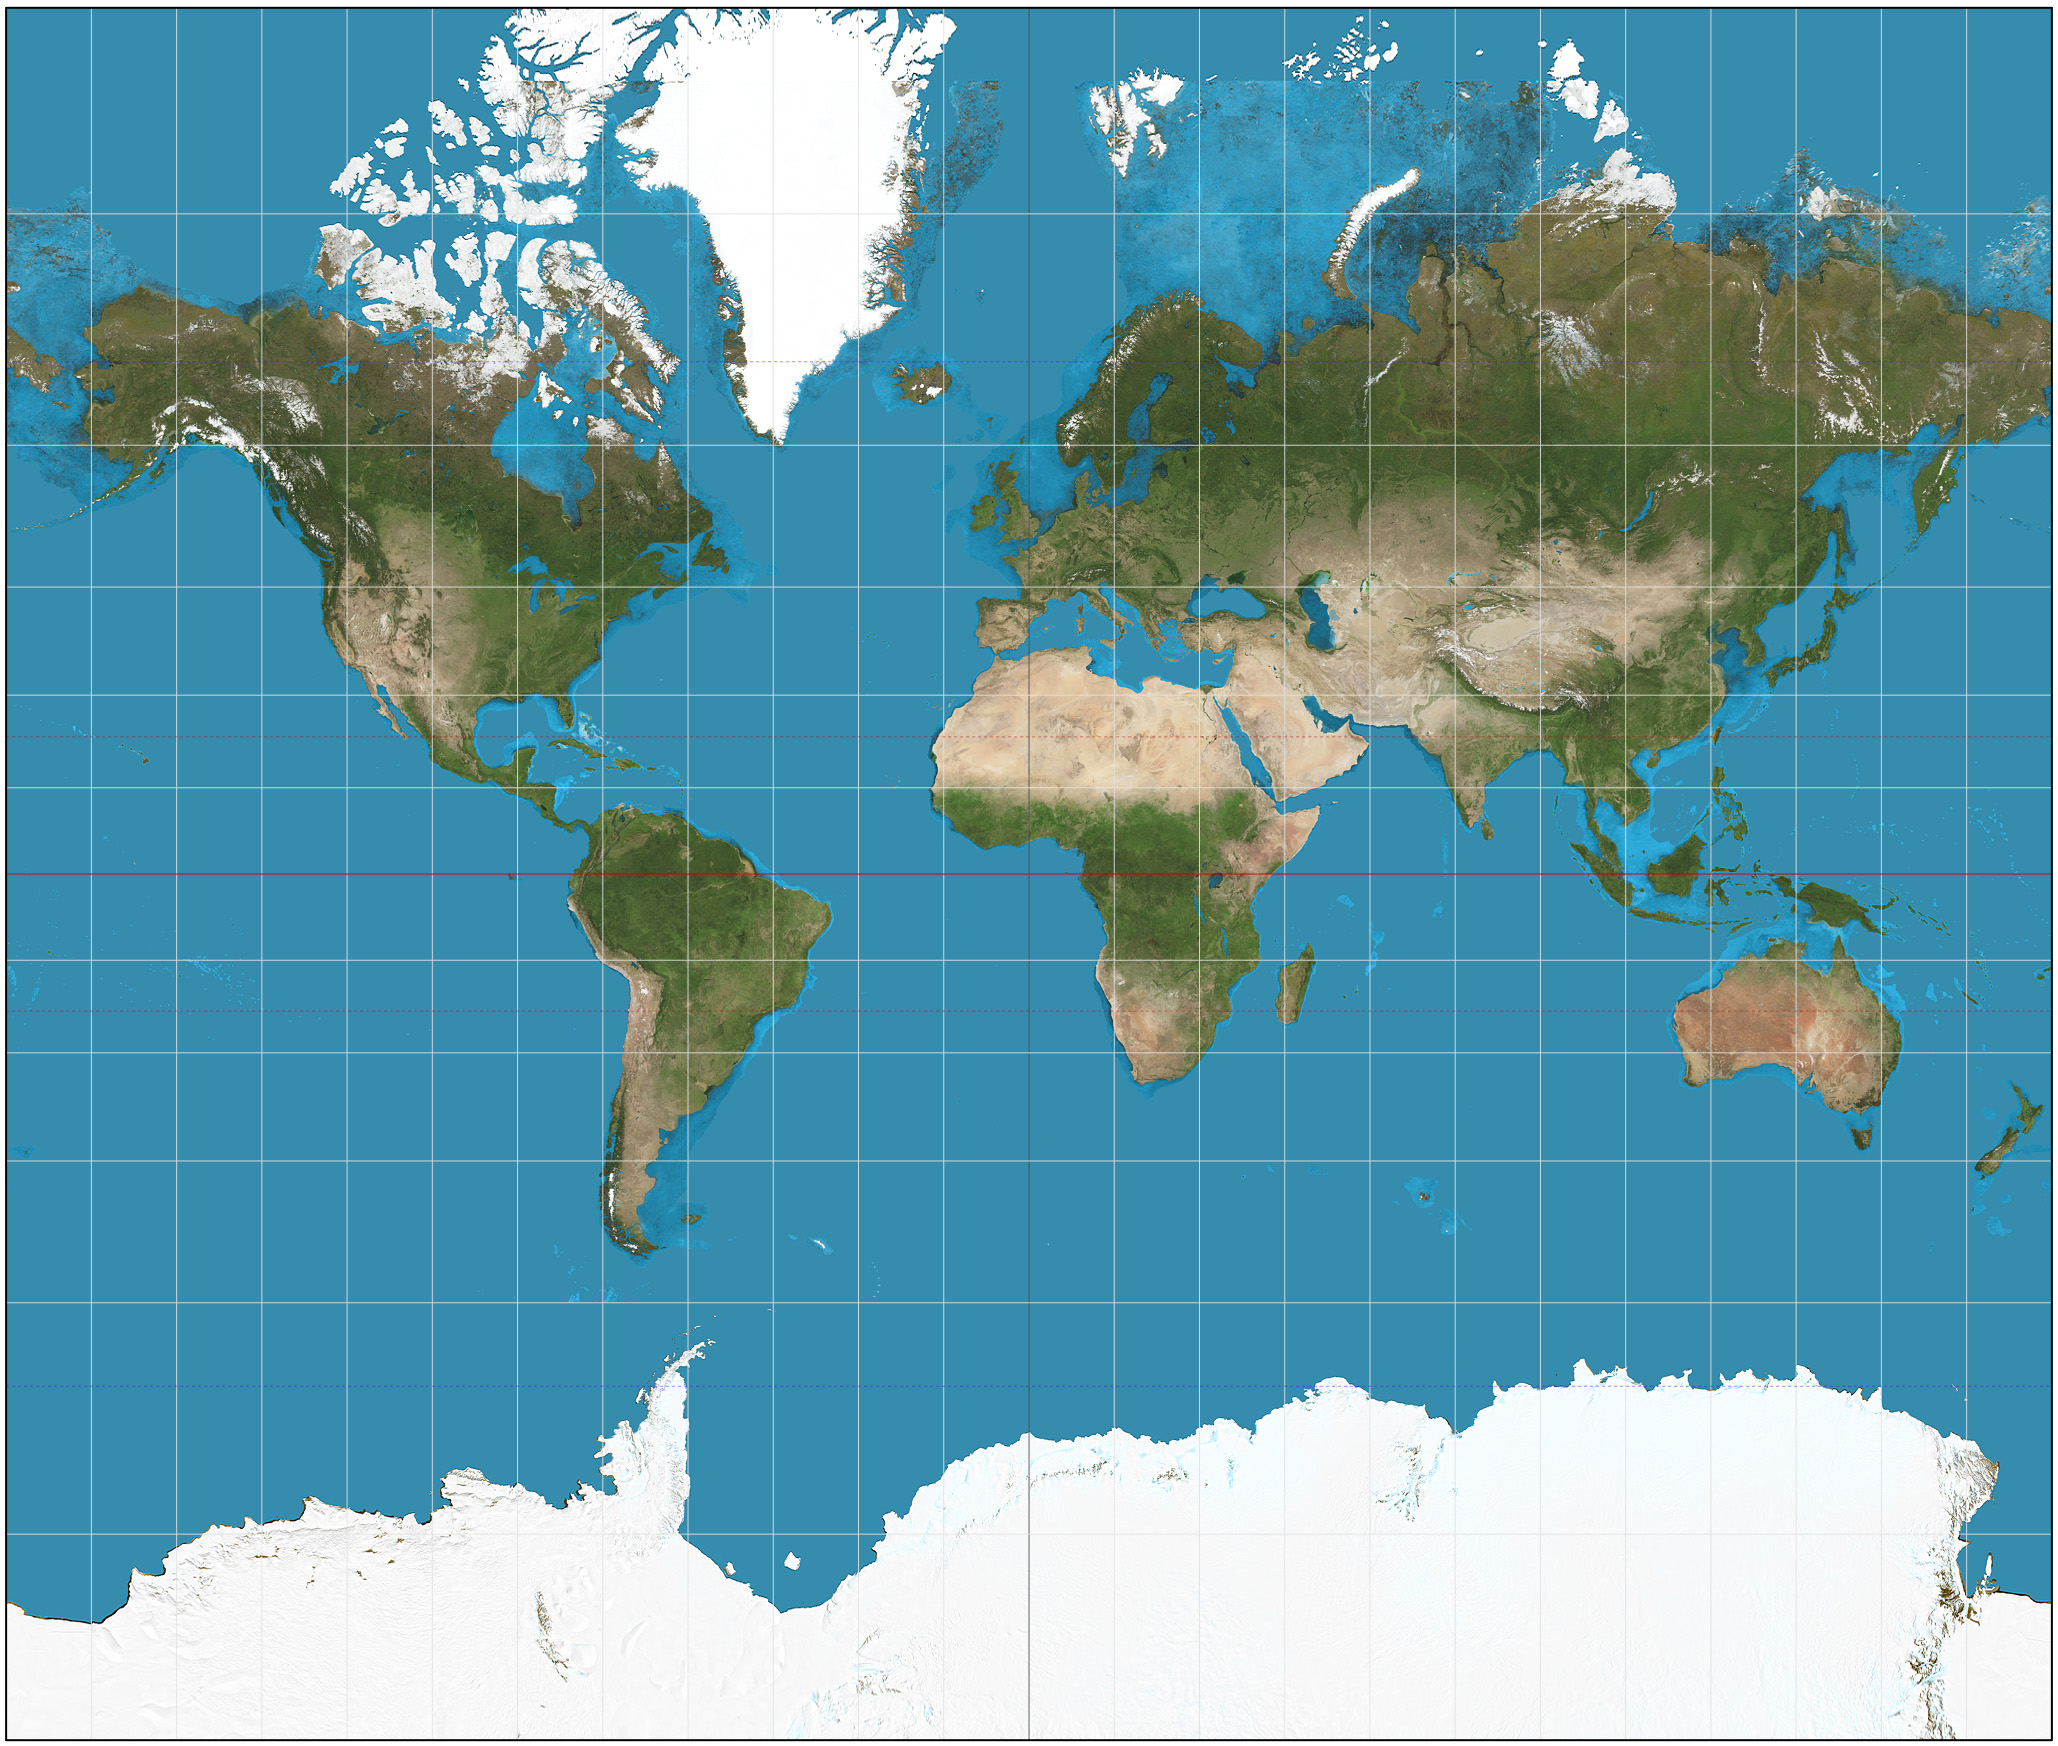
\includegraphics[width=.5\textwidth]{Images/Mercator_projection_SW.jpg}
    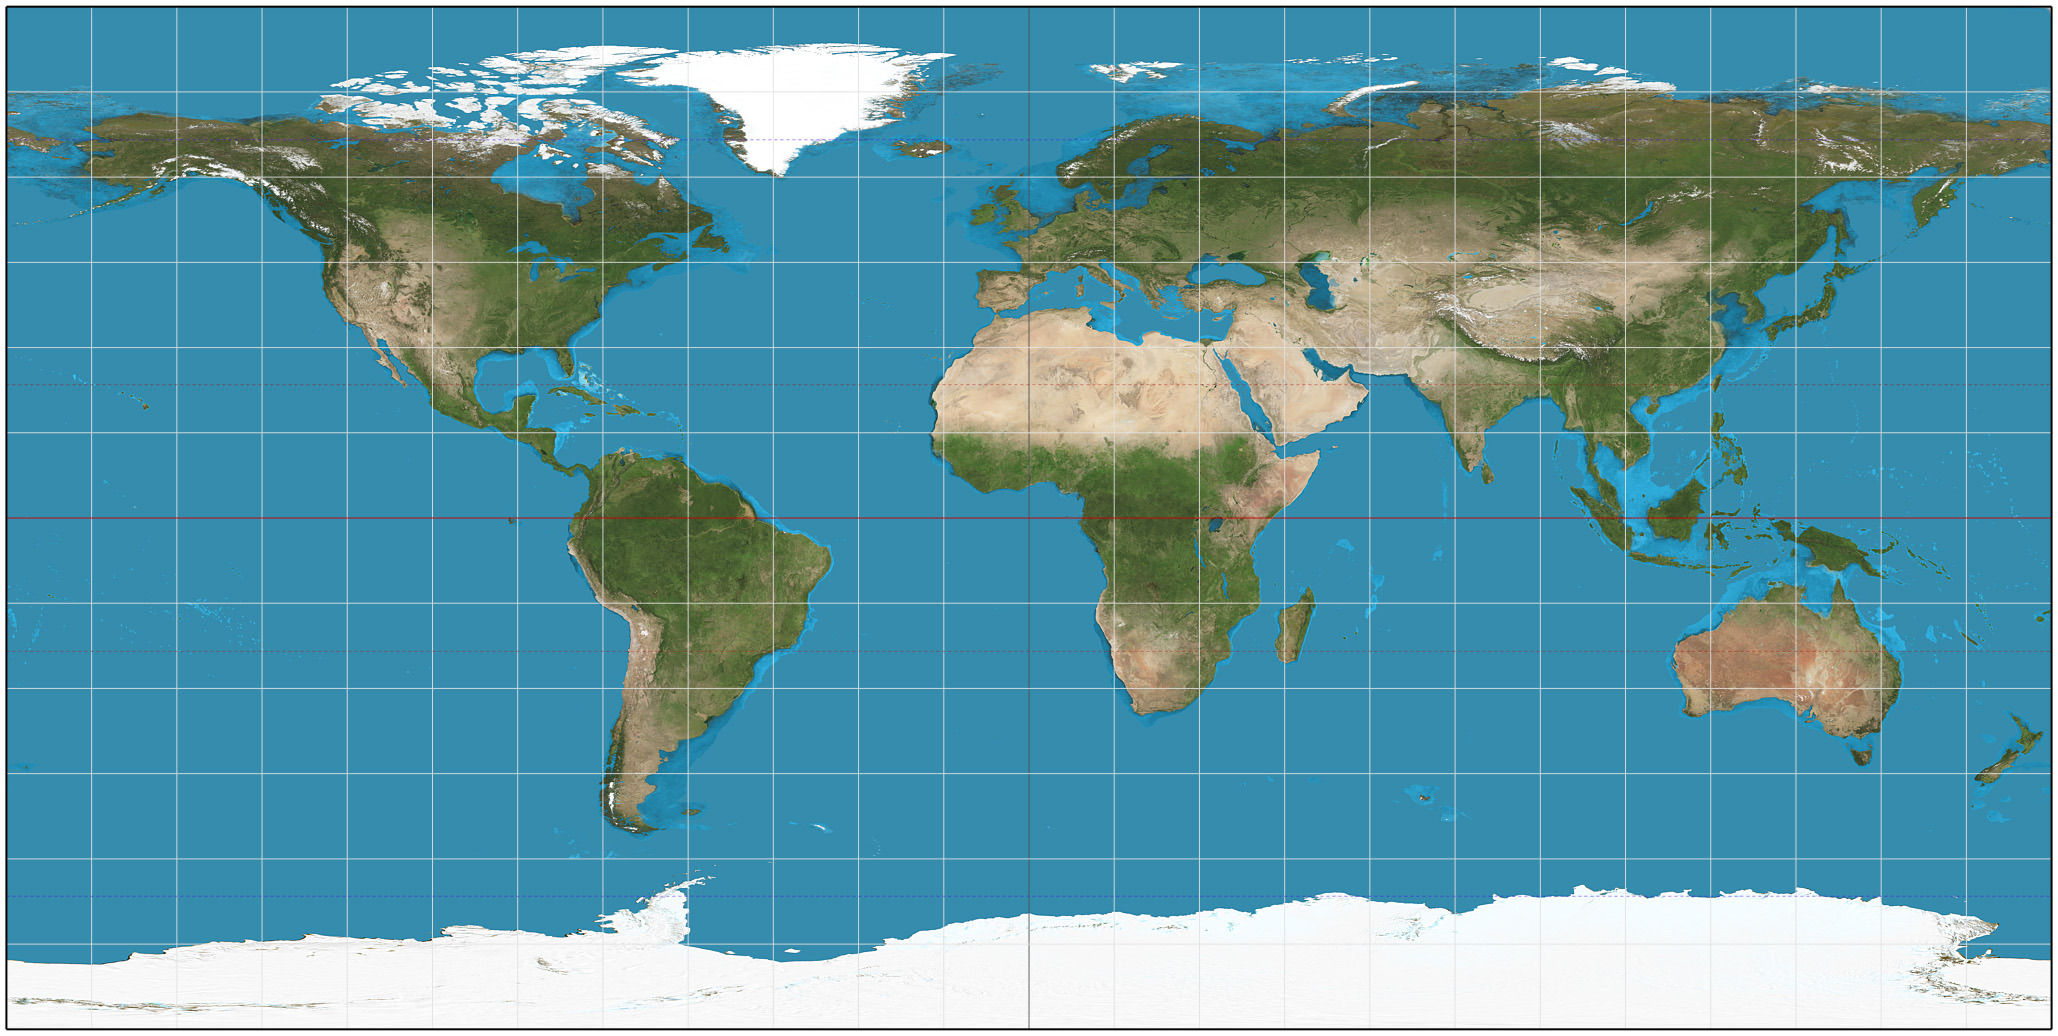
\includegraphics[width=.5\textwidth]{Images/Equirectangular_projection_SW.jpg}
\caption[]{Mercator projection(left) vs. Equirectangular projection(right)}
\label{fig:projections}
\end{figure}

In \cref{fig:projections} we can see, what we already described before.
In contrast to the Equirectangular projection on the right that looks quite swaged near the poles, the Mercator projection on the left stretches vertically in those parts, which leads to a much more natural looking map.
Nevertheless, the Equirectangular projection has the huge benefit, that no extra calculation is necessary to use it.
Therefore and due to the fact that the effect of the Mercator projection is quite low, we are going to use the Equirectangular projection for further work.


\paragraph{Edges}
At this point, we've already decided how to arrange the nodes on the screen.
That is why we can now think about a way to represent the basic elements of the graph, starting with the edges.
The most obvious characteristic of edges, is that they connect nodes.
Therefore the first thing that comes to mind, when thinking about drawing edges, which is also widely seen in graph visualizations, is to represent them by straight lines.
This might also be the best fit for our visualization, as it can be implemented without any bigger performance costs and even shows the length of the by the edge represented street quite well.\\
A possible improvement could still be achieved by displaying a more precise length and the other information we got about the edges, the speed.
An idea for showing a more precise length is, to bend the lines depending on the factor between the linear distance and the given length of two nodes.
The speed could be represented by coloring the lines.
For example, a slow edge could be colored red and a faster one green.\\
As clearness and comprehensibility is a major goal we want to achieve, we are going to stick with the simple single-colored, straight lines for now.


\paragraph{Nodes}
In most common visualizations of graphs nodes are represented as circles.
Those visualizations are mostly used for smaller graphs, which are used to explain the basic concepts of an algorithm.
Thus we should reconsider this representation of nodes, as we are also going to display graphs with millions of nodes.
Since we know that at the end of every edge is exactly one node, we can clearly identify every node, as long as the node is connected to any other edge.
Therefore we should consider to not add any additional representation of those nodes to the visualization as they do not add any value to it and only make the visualization more crowded.
But how to proceed with the remaining nodes?
As the only way for those nodes to play a role during our algorithm would be to be the start or the target node, we can just not visualize them for the sake of clarity.


\section{Displaying the Algorithm}

In this section, we are going to take a look on how to transform the representation a graph, as discussed in \cref{graph}, in a visualization of an algorithm.
The difference between the representation of a graph and the visualization of a graph algorithm is, that the visualization of an algorithm is a process which means that we want to display what is happening while the algorithm progresses.

\subsection{Basics}
For showing the process of the algorithm we are going to start with an empty space and then add one edge after another as they have been passed by the algorithm.
For a better highlighting of the last passed edge, we are going to highlight this specific edge.

\begin{figure}[H]
    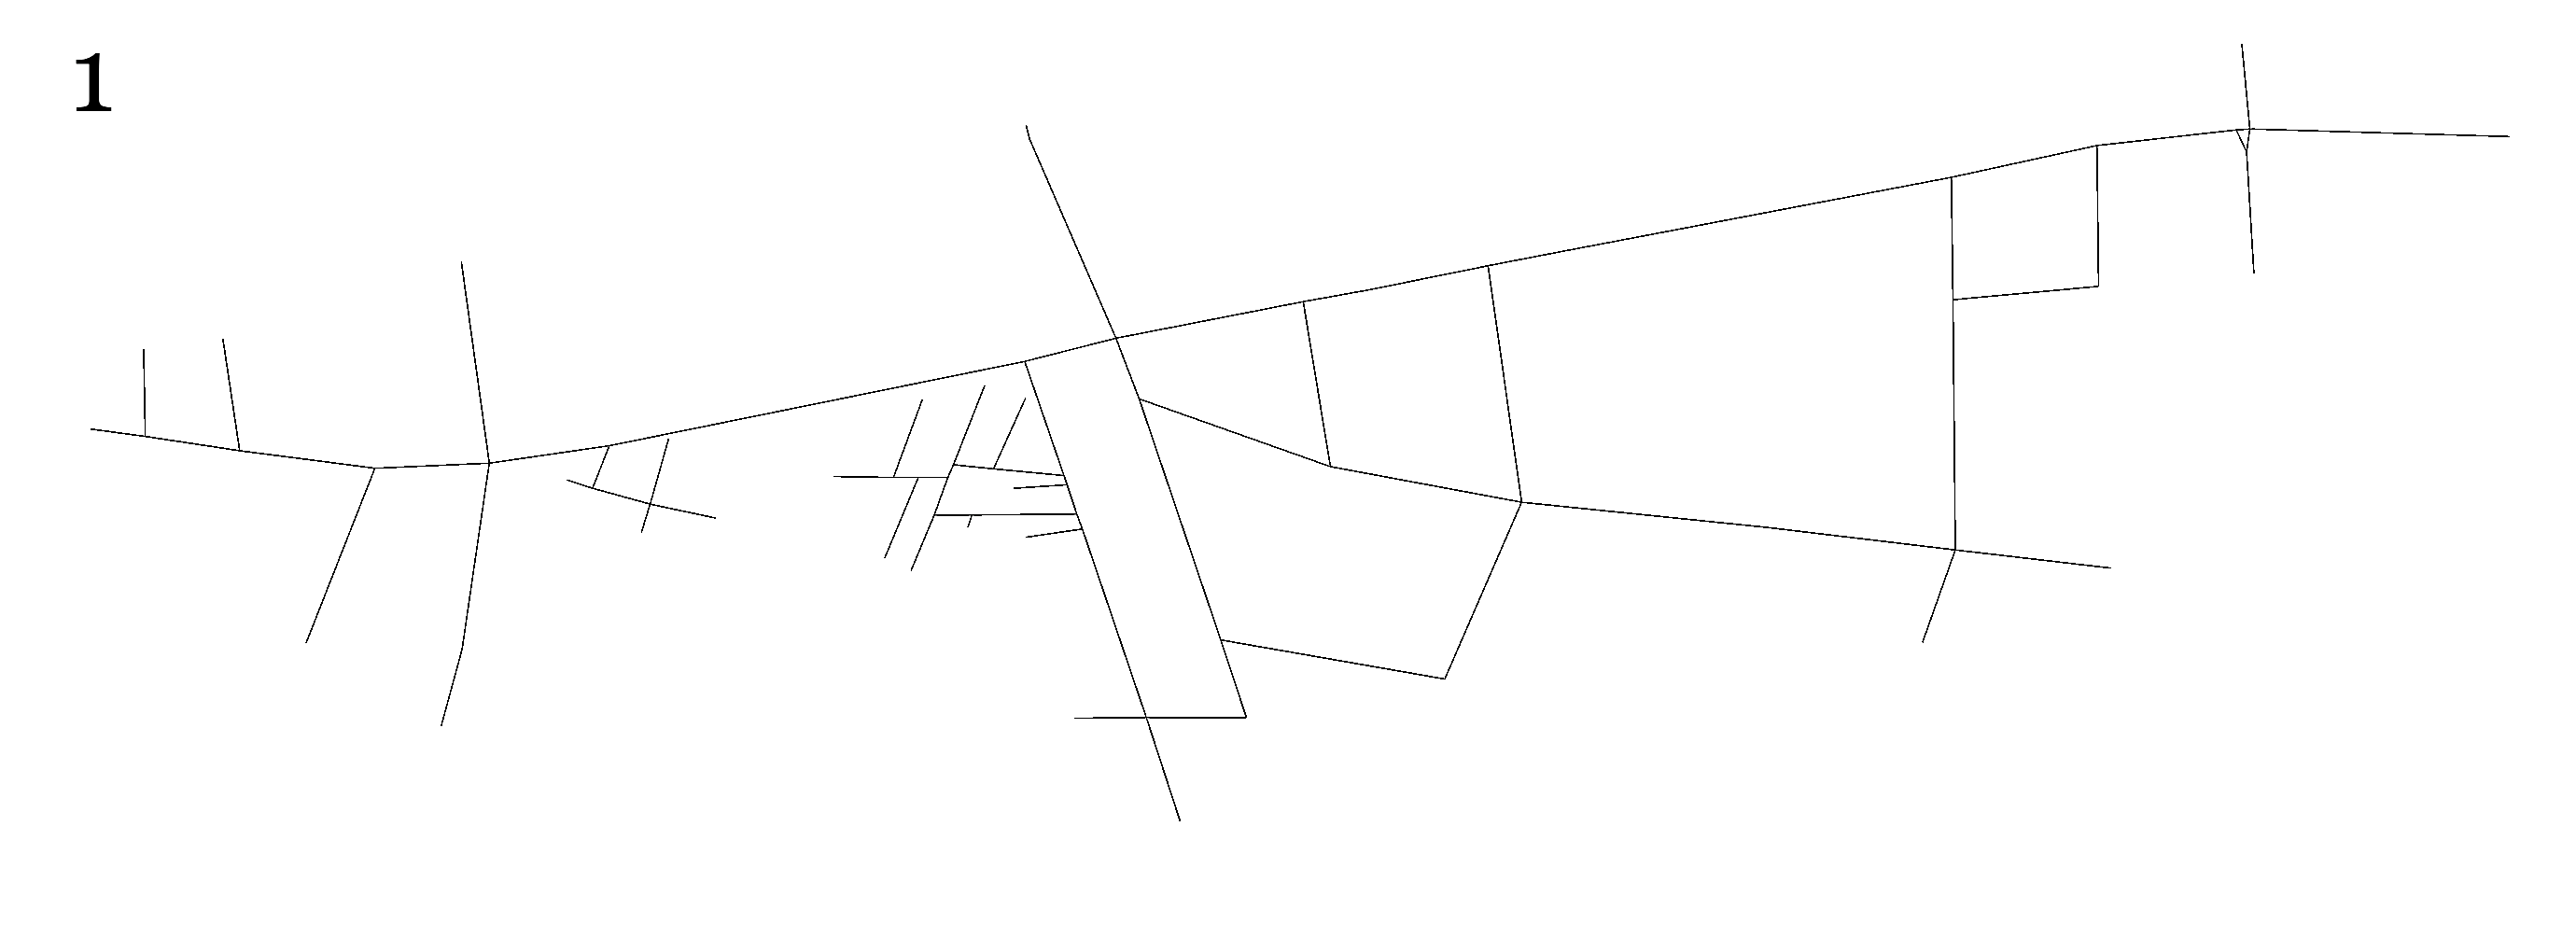
\includegraphics[width=.5\textwidth]{Images/vis-step-one.png}
    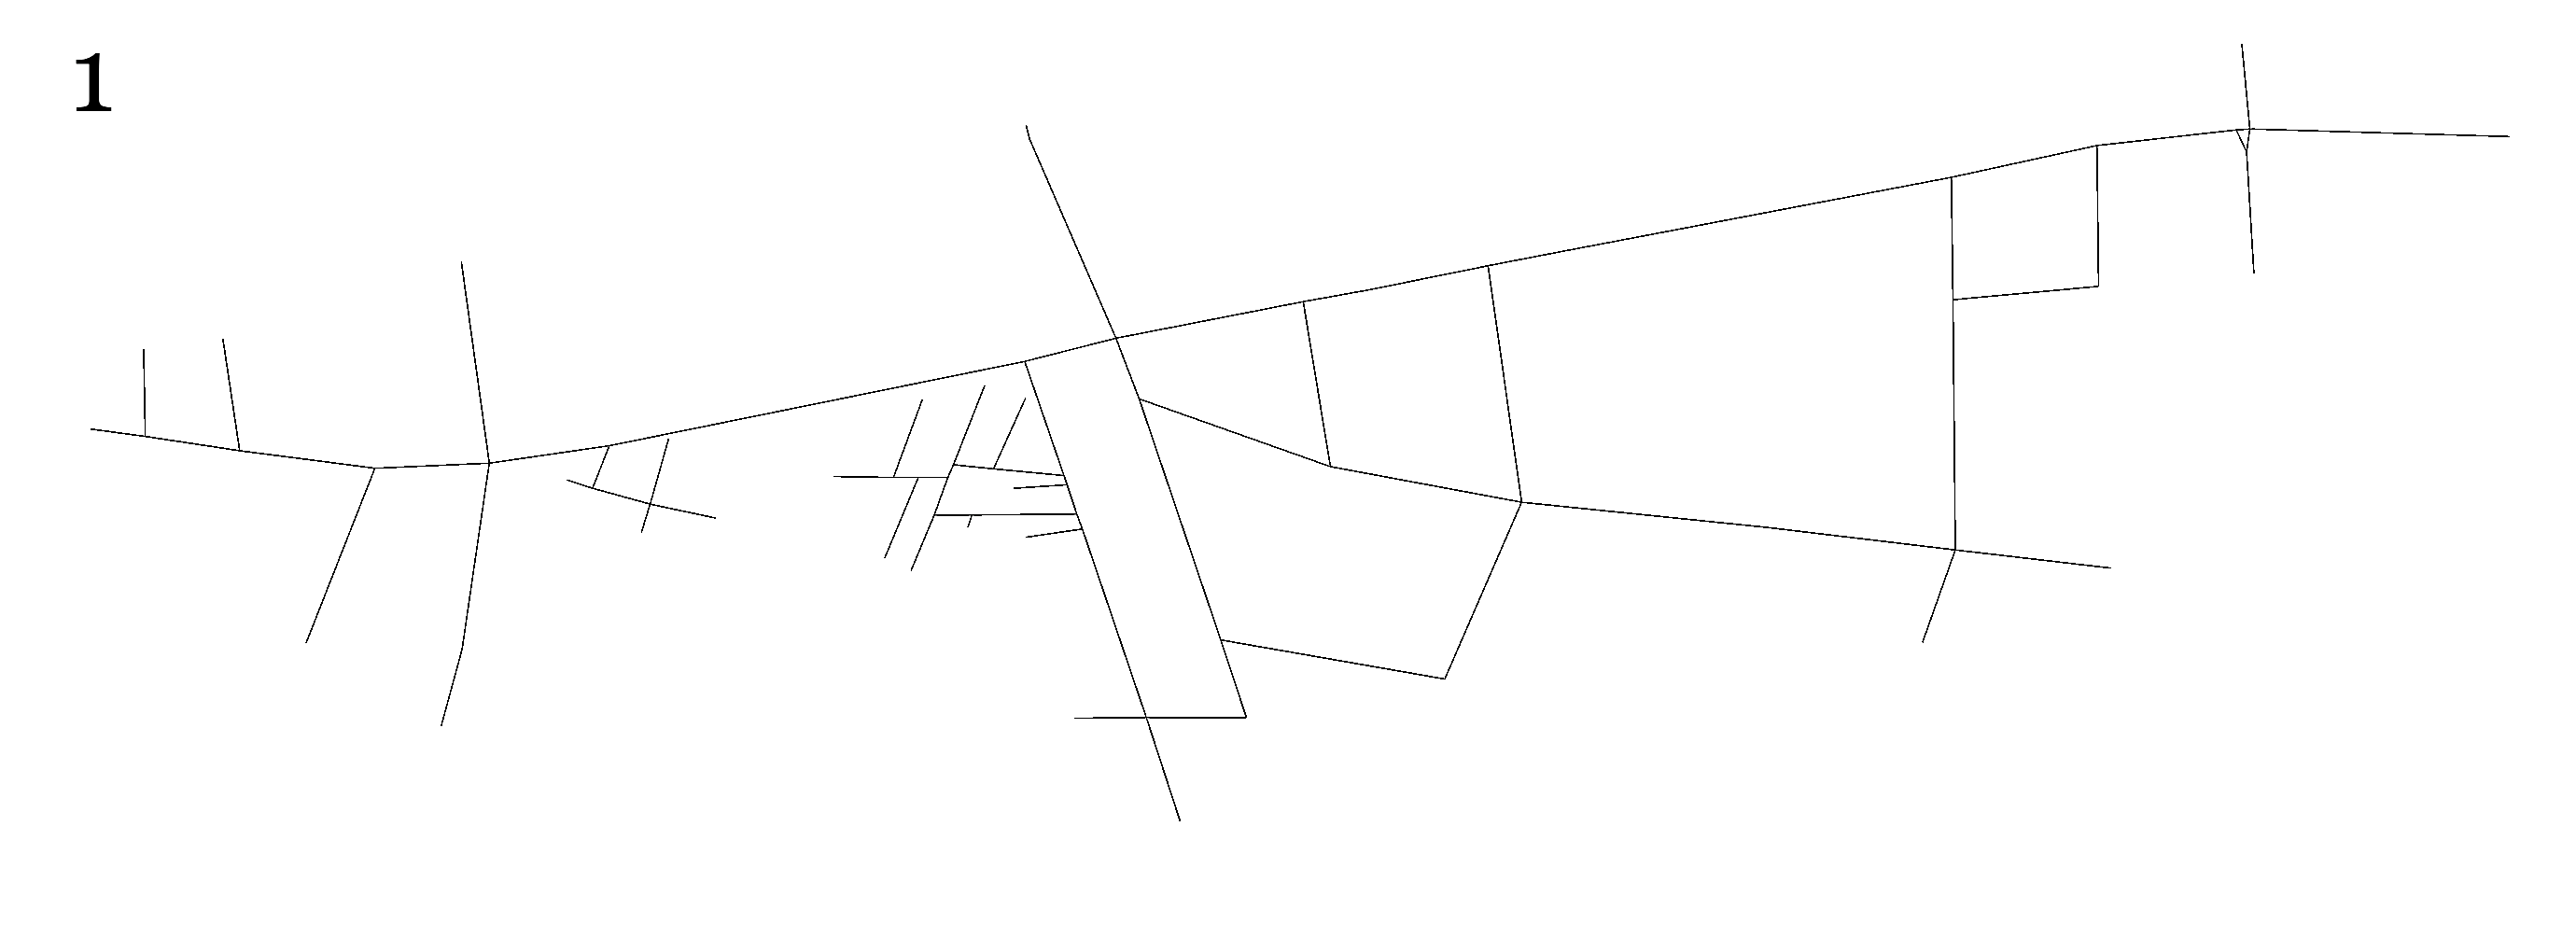
\includegraphics[width=.5\textwidth]{Images/vis-step-one.png}
\caption[]{Two consecutive steps in the visualization. Every black line represents an edge and the last processed edge is colored blue.}
\label{fig:two-steps}
\end{figure}

In \cref{fig:two-steps} we can see that we get a good understanding of how the algorithm evolves.
We will now add the shortest path that was by the algorithm.
Thereby we know at any point where the start and target nodes of the algorithm are and how far the algorithm is finding the shortest path.

\begin{figure}[H]
 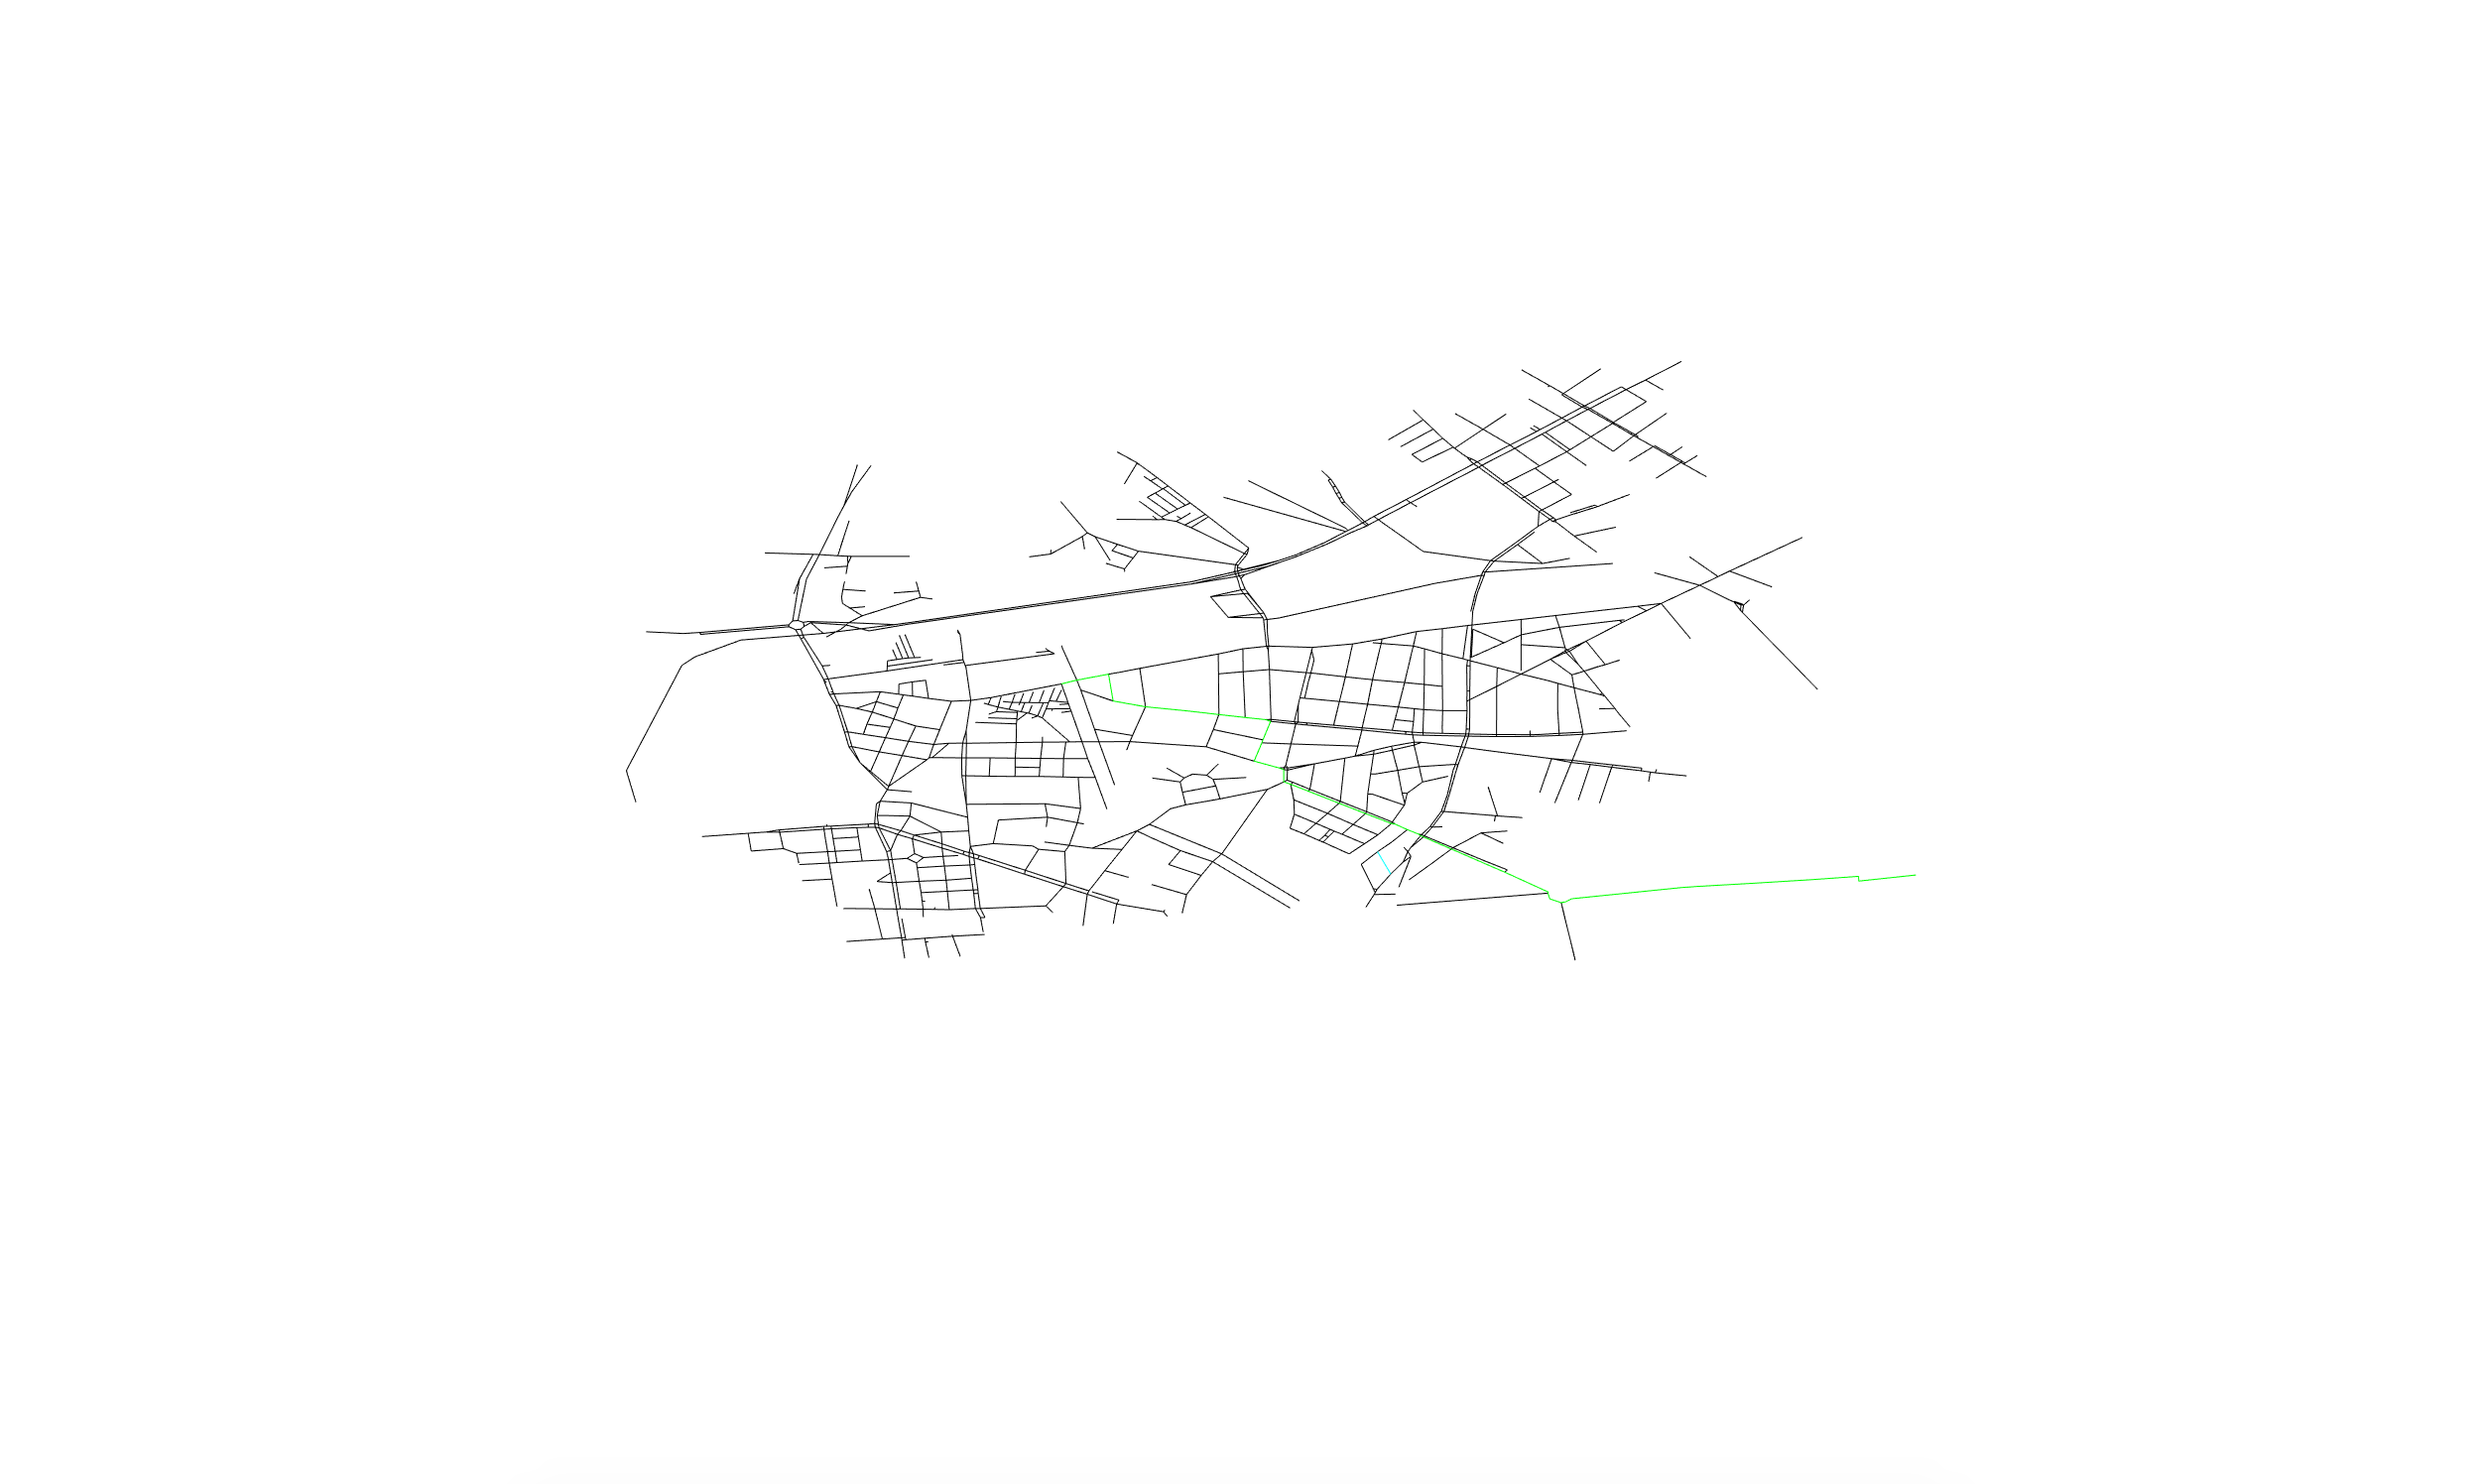
\includegraphics[width=\textwidth]{Images/vis-result-path.png}
\caption[]{Adding the final path to the visualization. Represented by the green line.}
\label{fig:result-path}
\end{figure}

At this point, we will have to think about where we want to place the edges on the screen.
As the displayed graph grows as the algorithm progresses there is the risk of growing out of the screen when we estimate the final graph too small.
On the other side, we could also estimate the graph to big, which would result in much unused space on out screen.\\
We will now have the choice to either try to estimate the extent of the explored graph of the fully evolved algorithm or iterate over the algorithm before visualizing it, for finding out its borders.
By iterating over the whole algorithm we would find out the exact borders of the graph we want to show.
With this knowledge about we could then adjust the size of the fully evolved graph flush with the borders of our visualization on two sides.

\begin{figure}[H]
    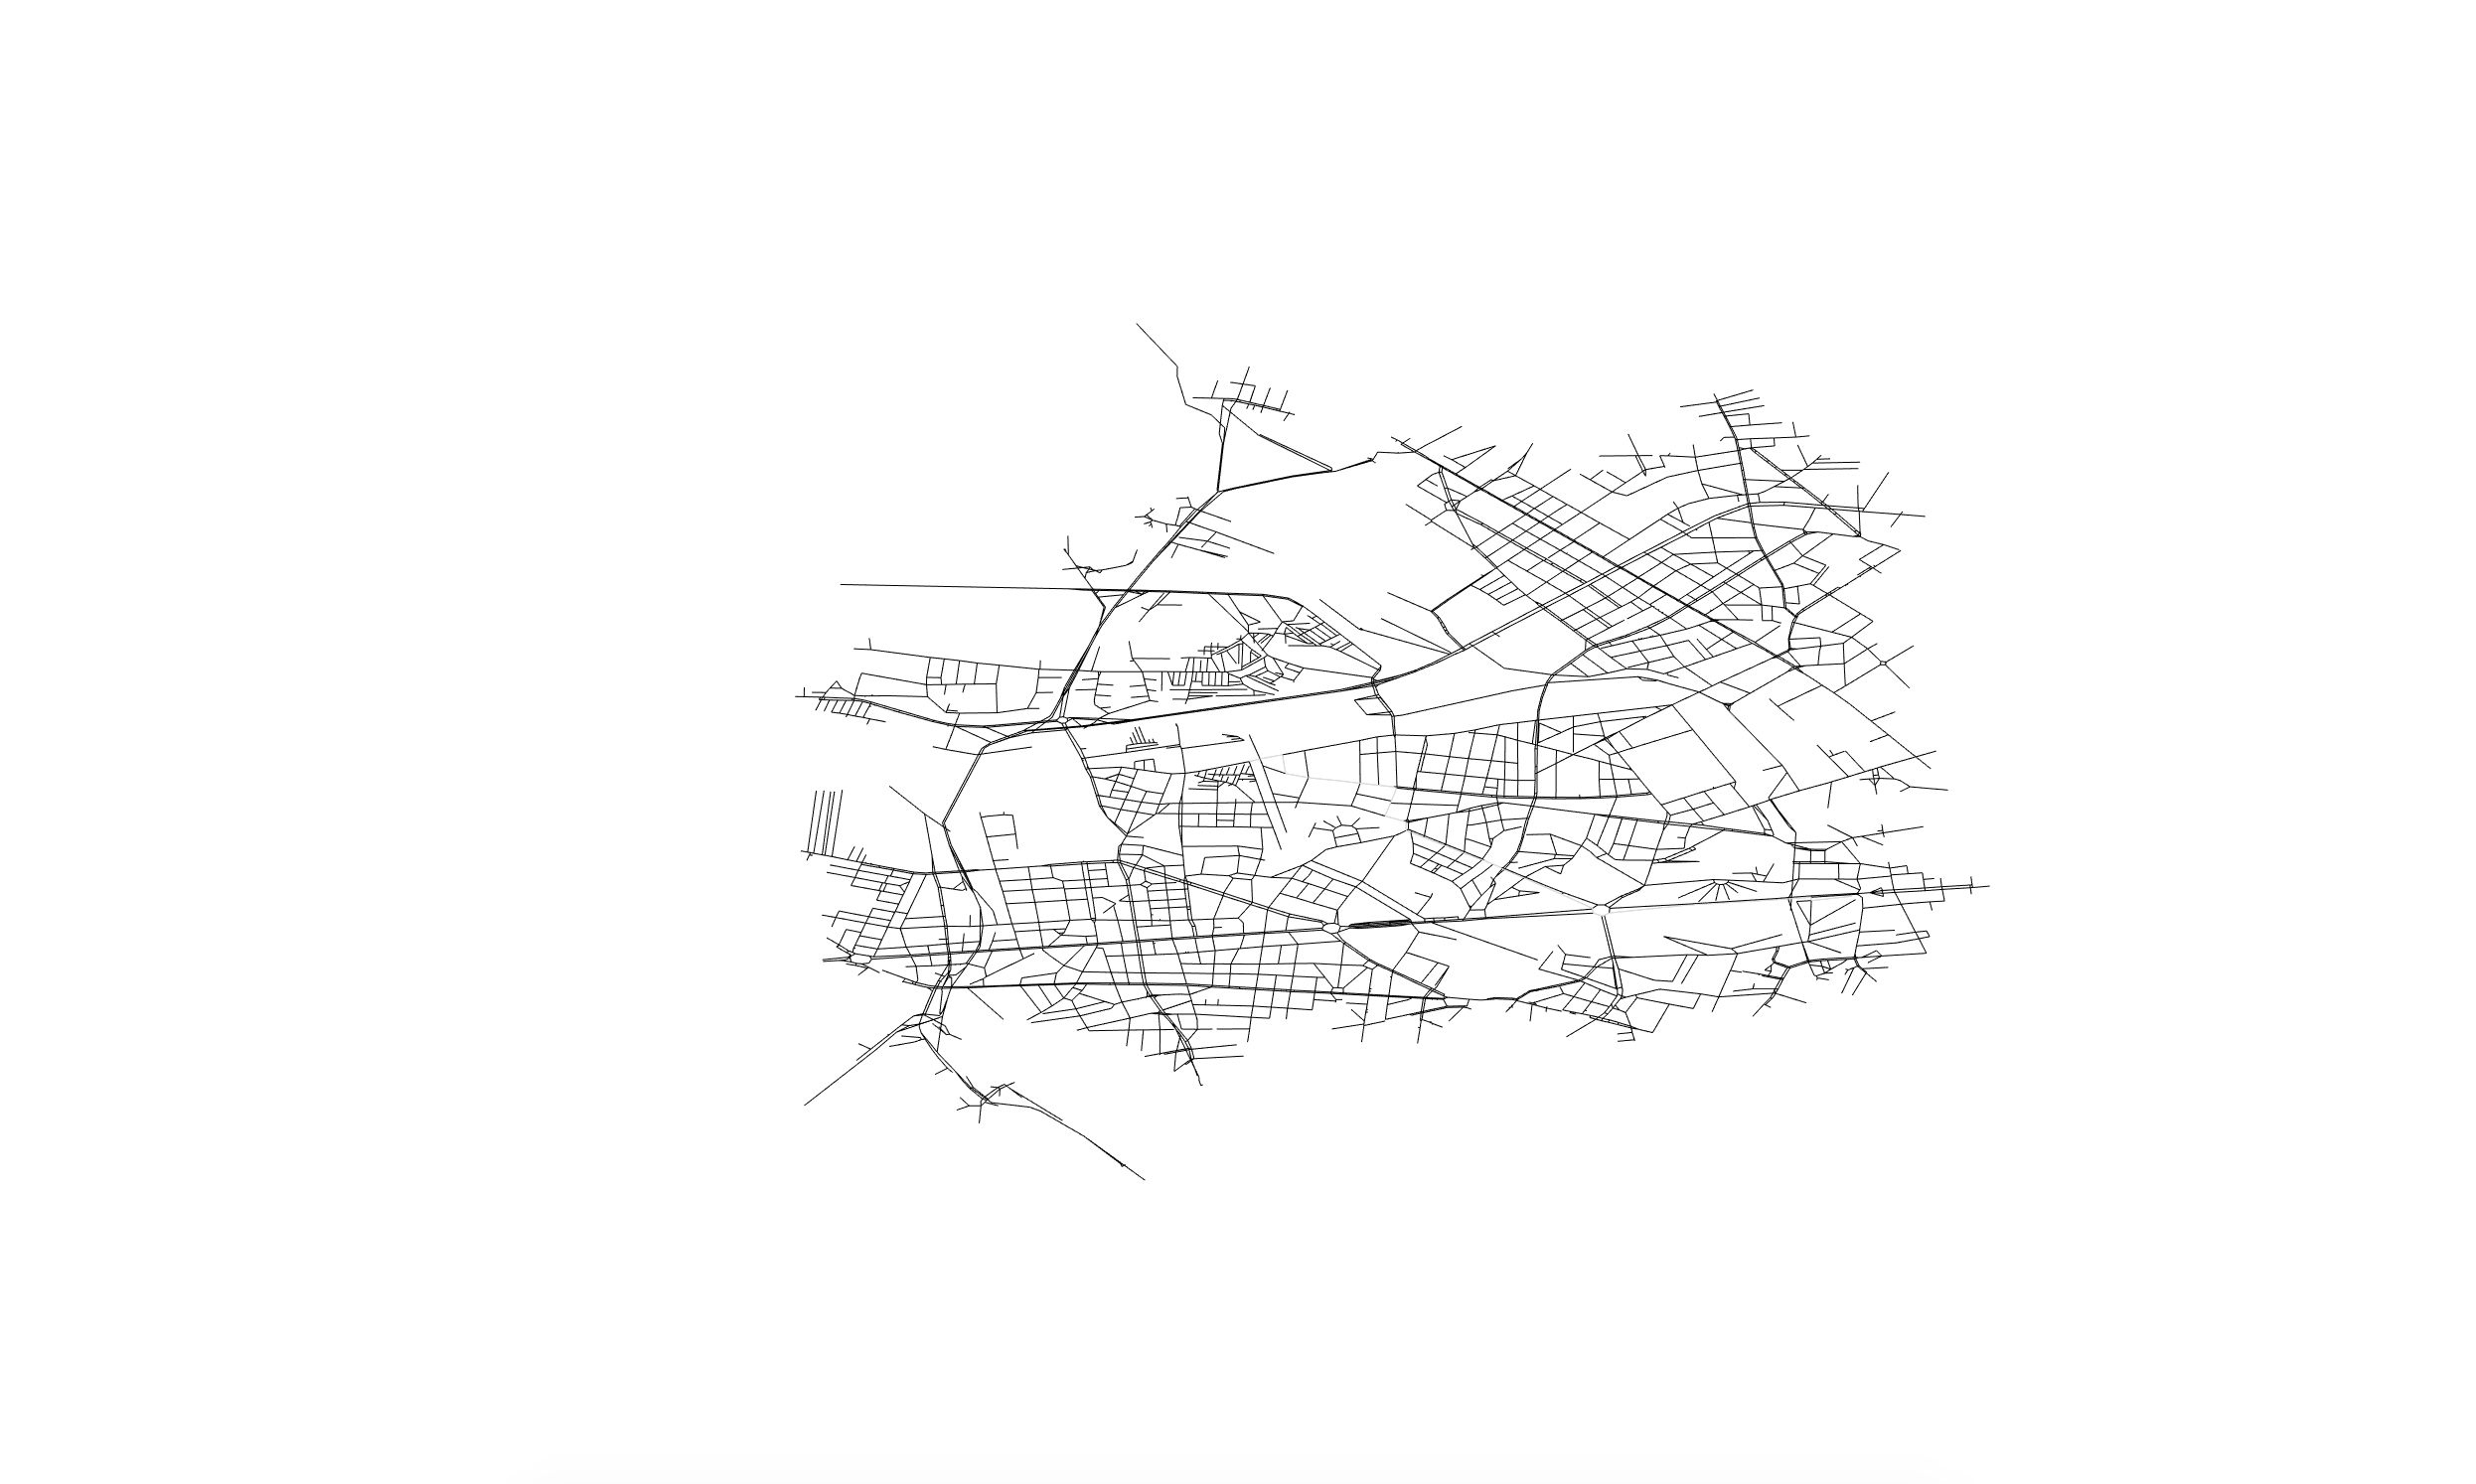
\includegraphics[width=.5\textwidth]{Images/vis-estimation.png}
    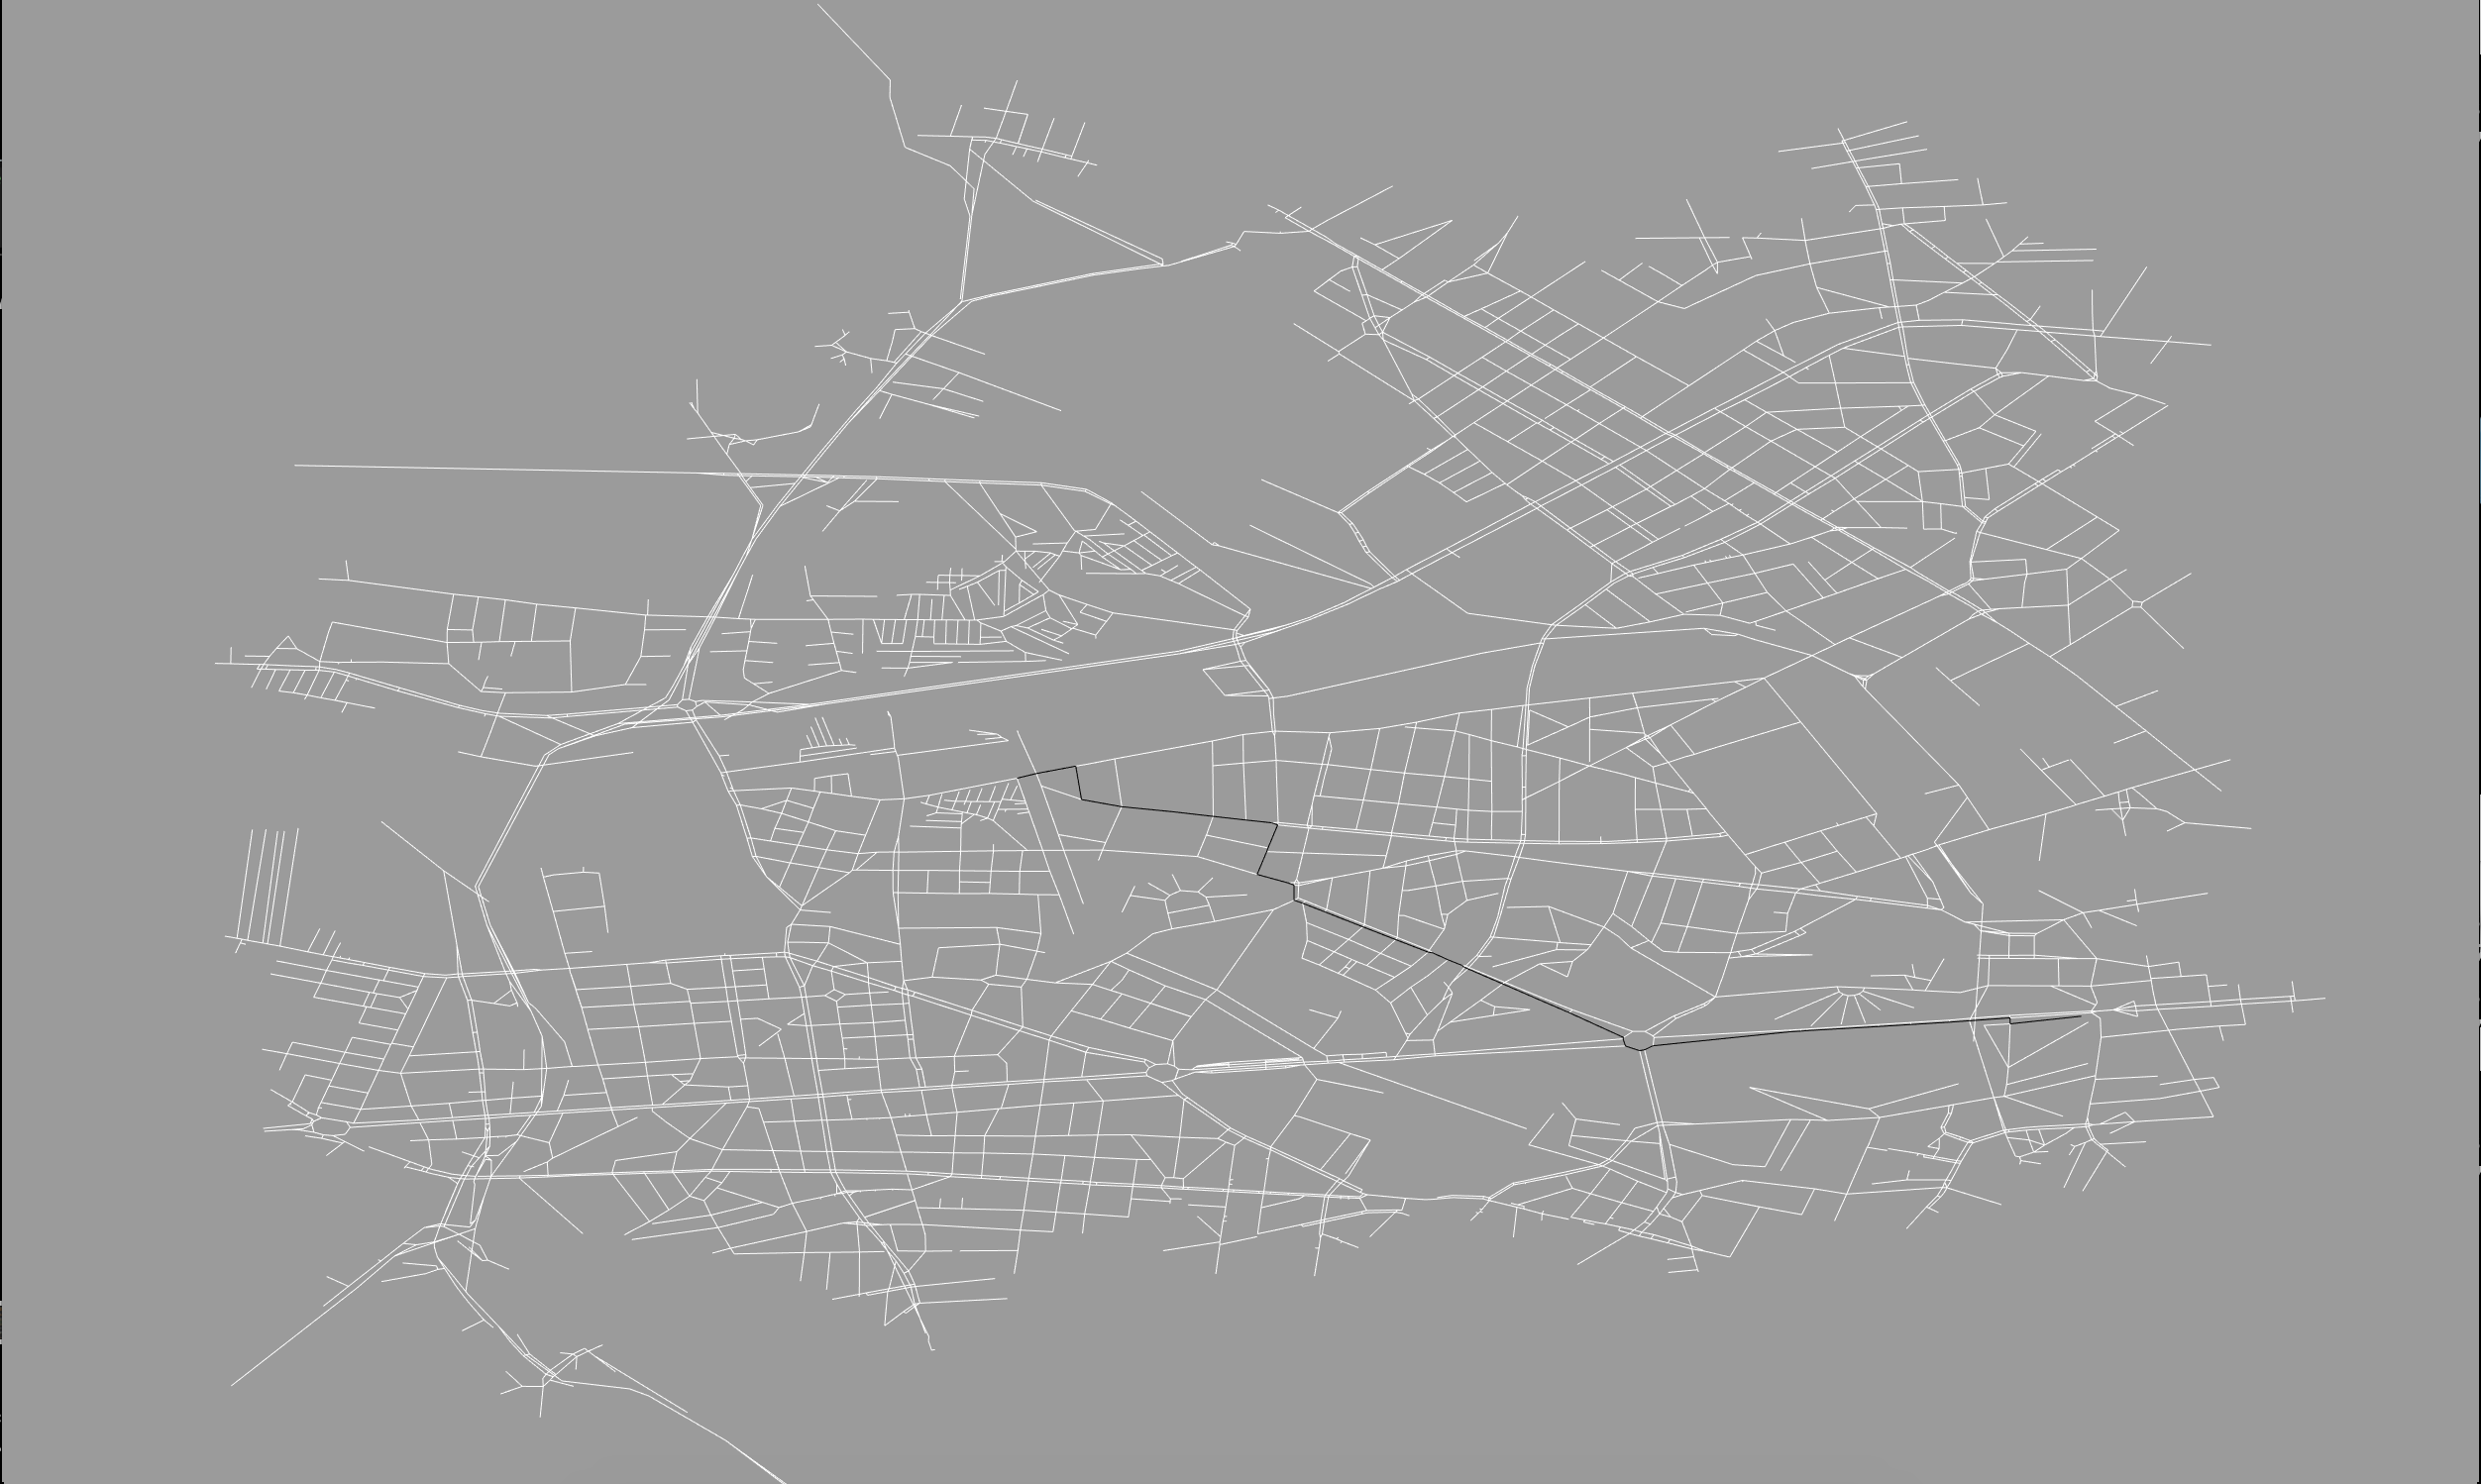
\includegraphics[width=.5\textwidth]{Images/vis-preprocessing.png}
\caption[]{Estimation method with quite a good estimation(left) vs. Preprocessing method(right)}
\label{fig:sections}
\end{figure}

The difference between those two cutouts is wuite big, as we see in \cref{fig:sections}.
For the shown estimation we used the linear distance between start and target node as the basis.
Thereby we made sure that the visualization shows everything that is happening in a radius of a little more than the linear distance between start and target node around the start node.
Even though this estimation was quite generous, we can never be sure that we get the whole graph on the screen when estimating.
In genreal better estimations are possible as well, but the better we would like the estimation to be, the more information we would need about the algorithm we show and the underlying graph, which we want to avoid.
Therefore we are going to continue using the preprocessing method for estimating the window we are going to show.\\

Now that we found the section we want to display, there would still be a possibility to minimize the empty space on our screen.
Currently, we are using the same scale on both axes.
This means that there could be a bigger empty space on one axis.
What we could do now is to change the scale on one of the axes and thereby spread the graph over the whole screen.

\begin{figure}[H]
    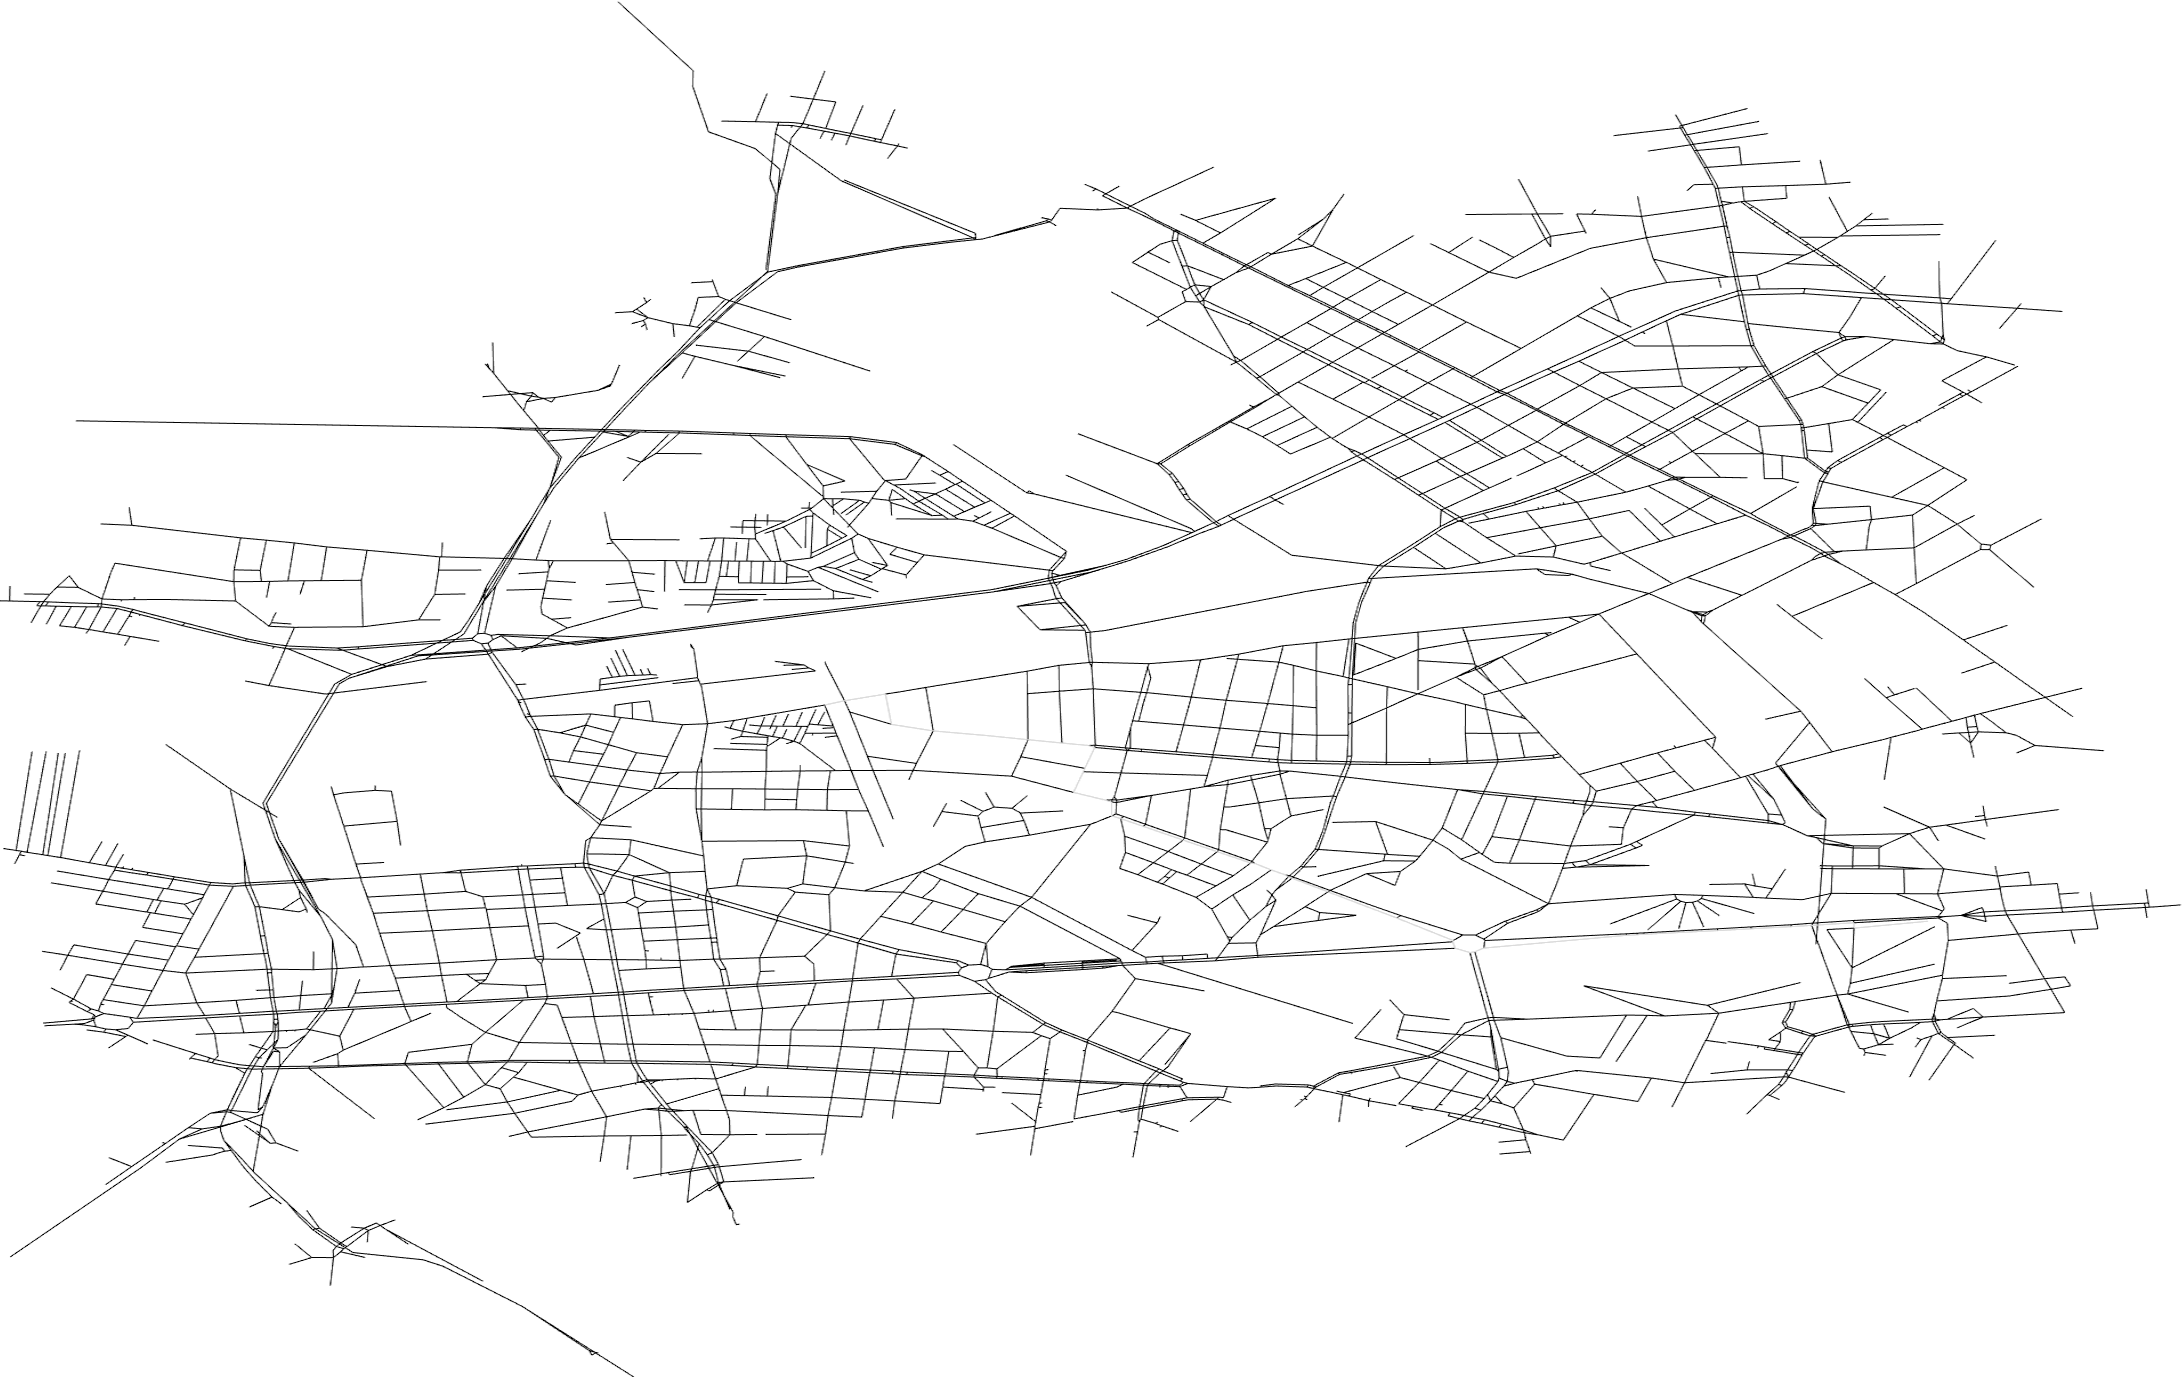
\includegraphics[width=\textwidth]{Images/vis-preprocessing-streched.png}
\caption[]{Preprocessing method with additional streching to the borders of the visualization}
\label{fig:spreaded_axis}
\end{figure}

As we see in \cref{fig:spreaded_axis} this reduces the unused space to a minimum.
Though we would loose a lot of understandability, as the length of a line on the screen would indicate the length of the real edge even less.
Therefore uniform scaled axes are the better choice for our graph visualization.


\subsection{Displaying the Tiles} \label{tiles}

In \cref{specification} we described that the graph is split into tiles, which due to their encryption and compression should be loaded as rarely as possible.
Therefore the tiles are the major cost factor during the algorithm and thus should be respected in the visualization.
A first idea for doing this is to display all edges of a tile as soon as a node of this tile has been accessed the first time.

\begin{figure}[H]
    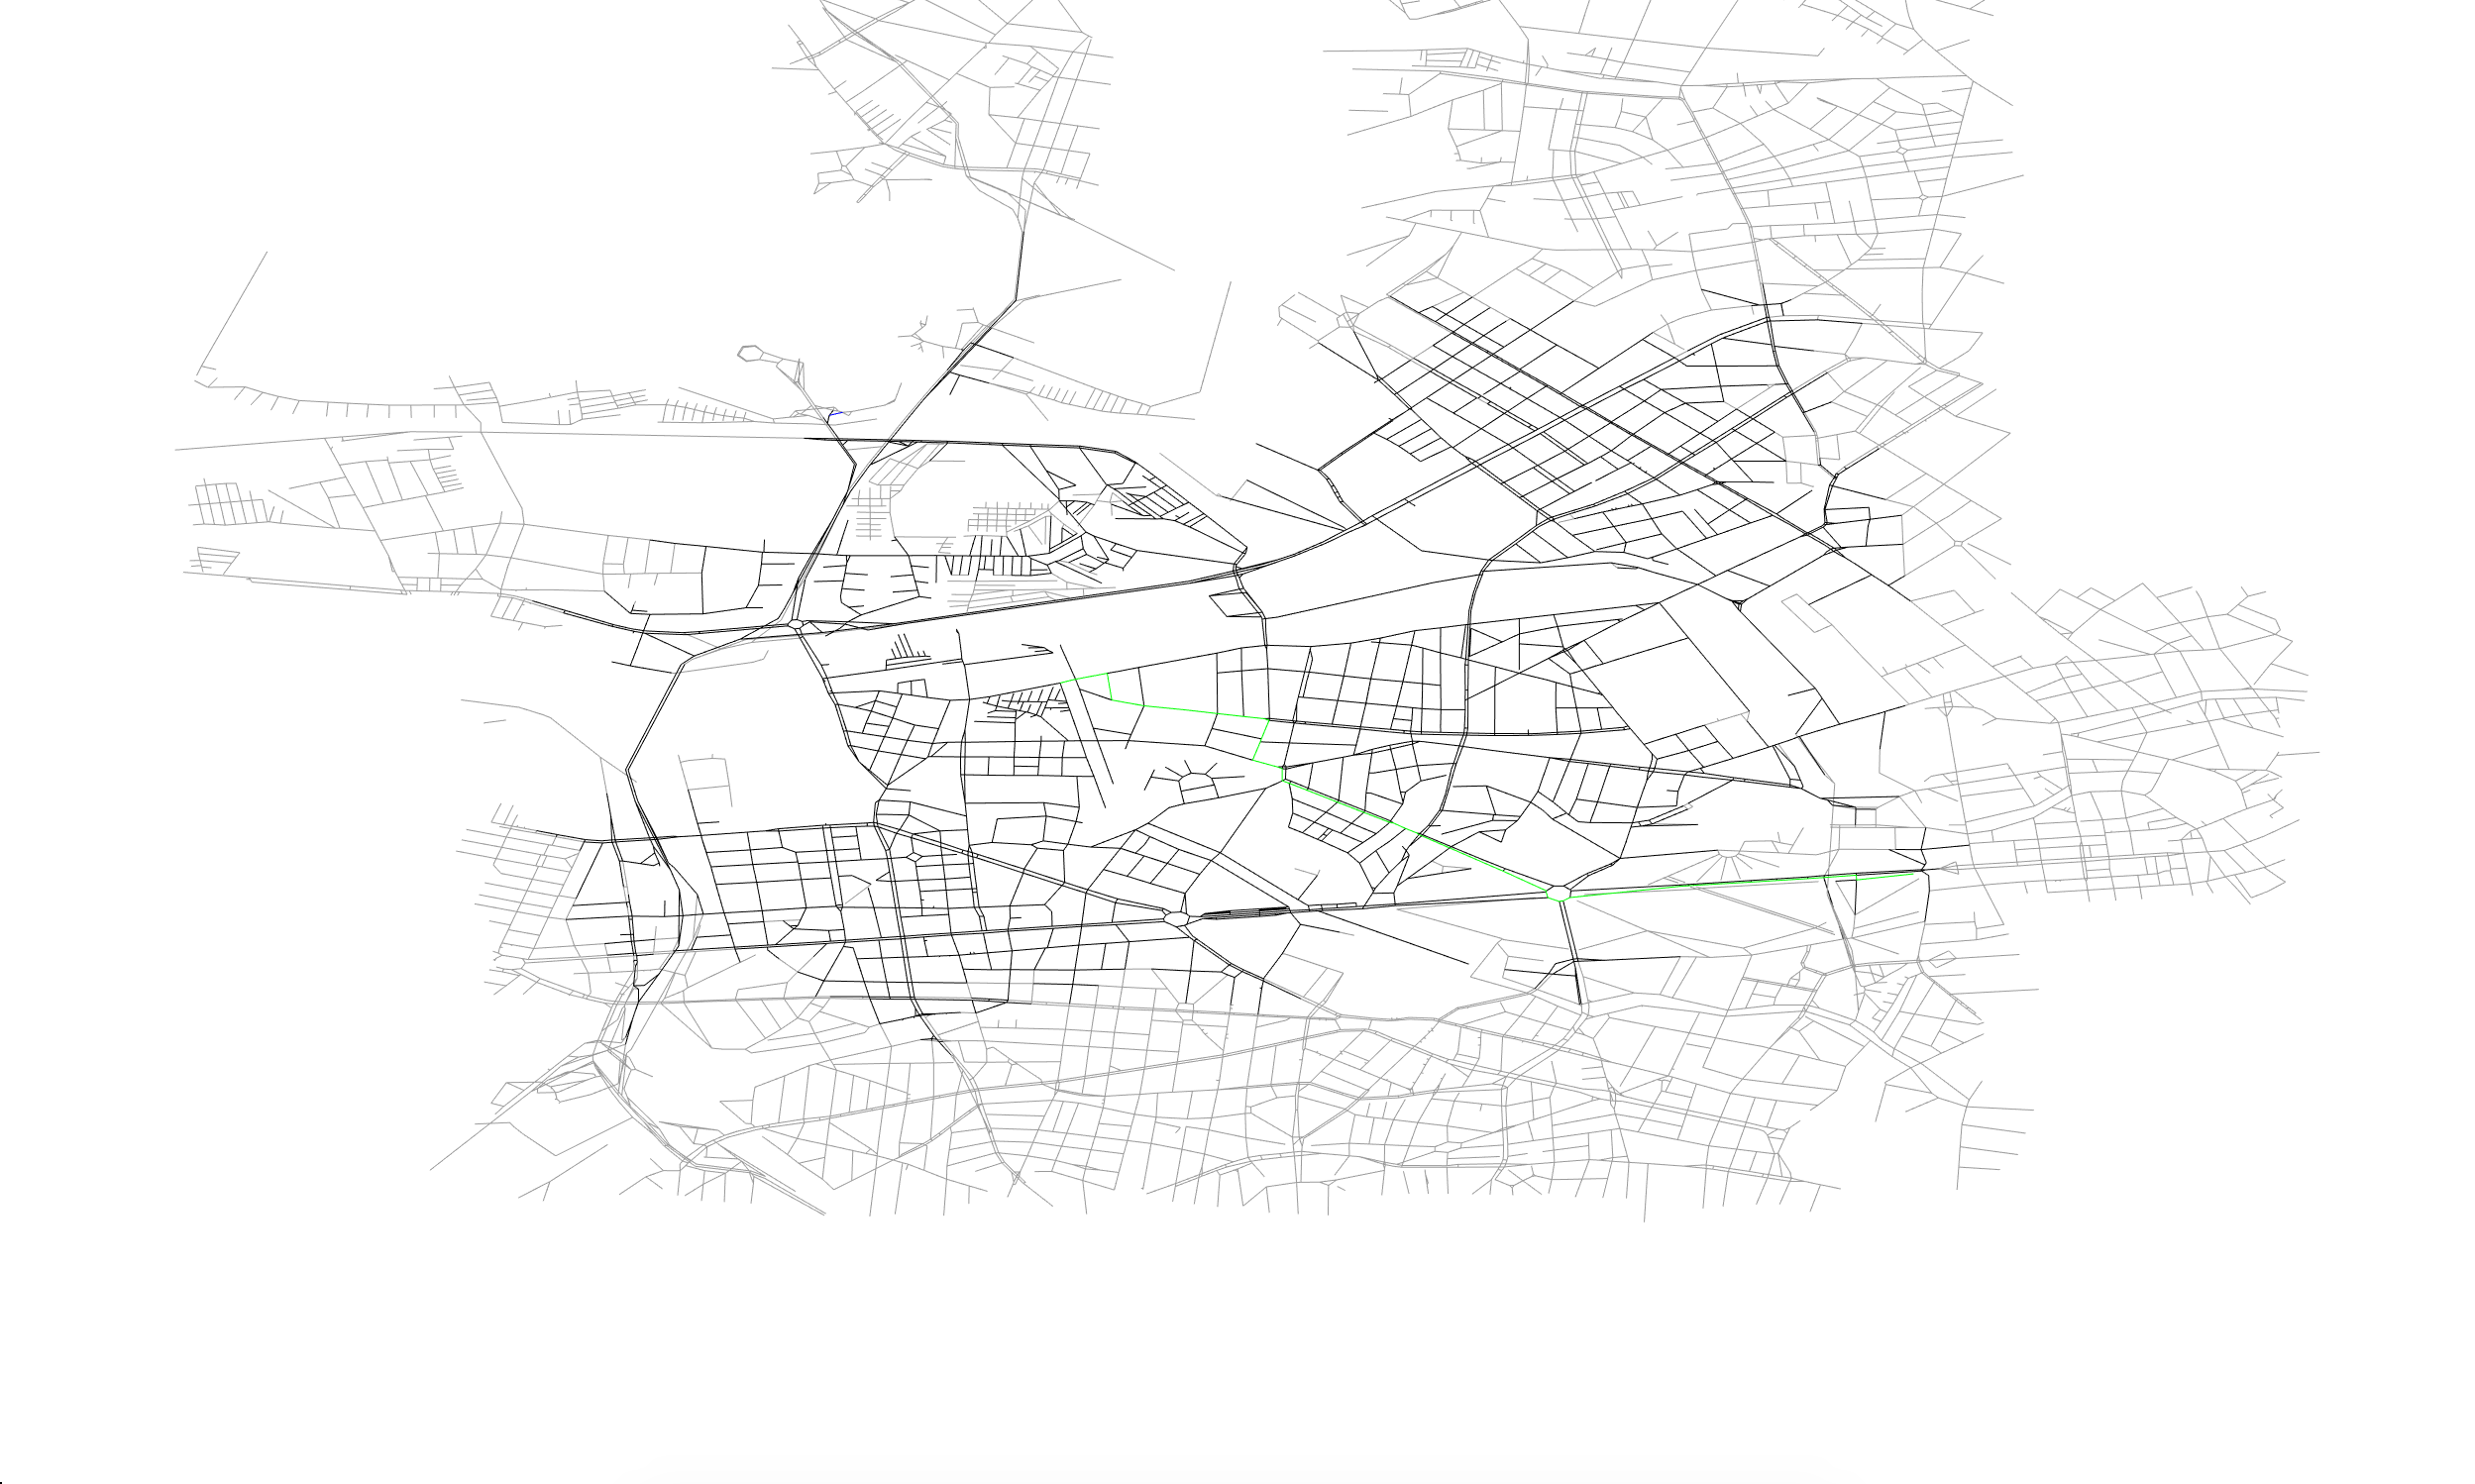
\includegraphics[width=0.5\textwidth]{Images/vis-tile-blocks-small.png}
    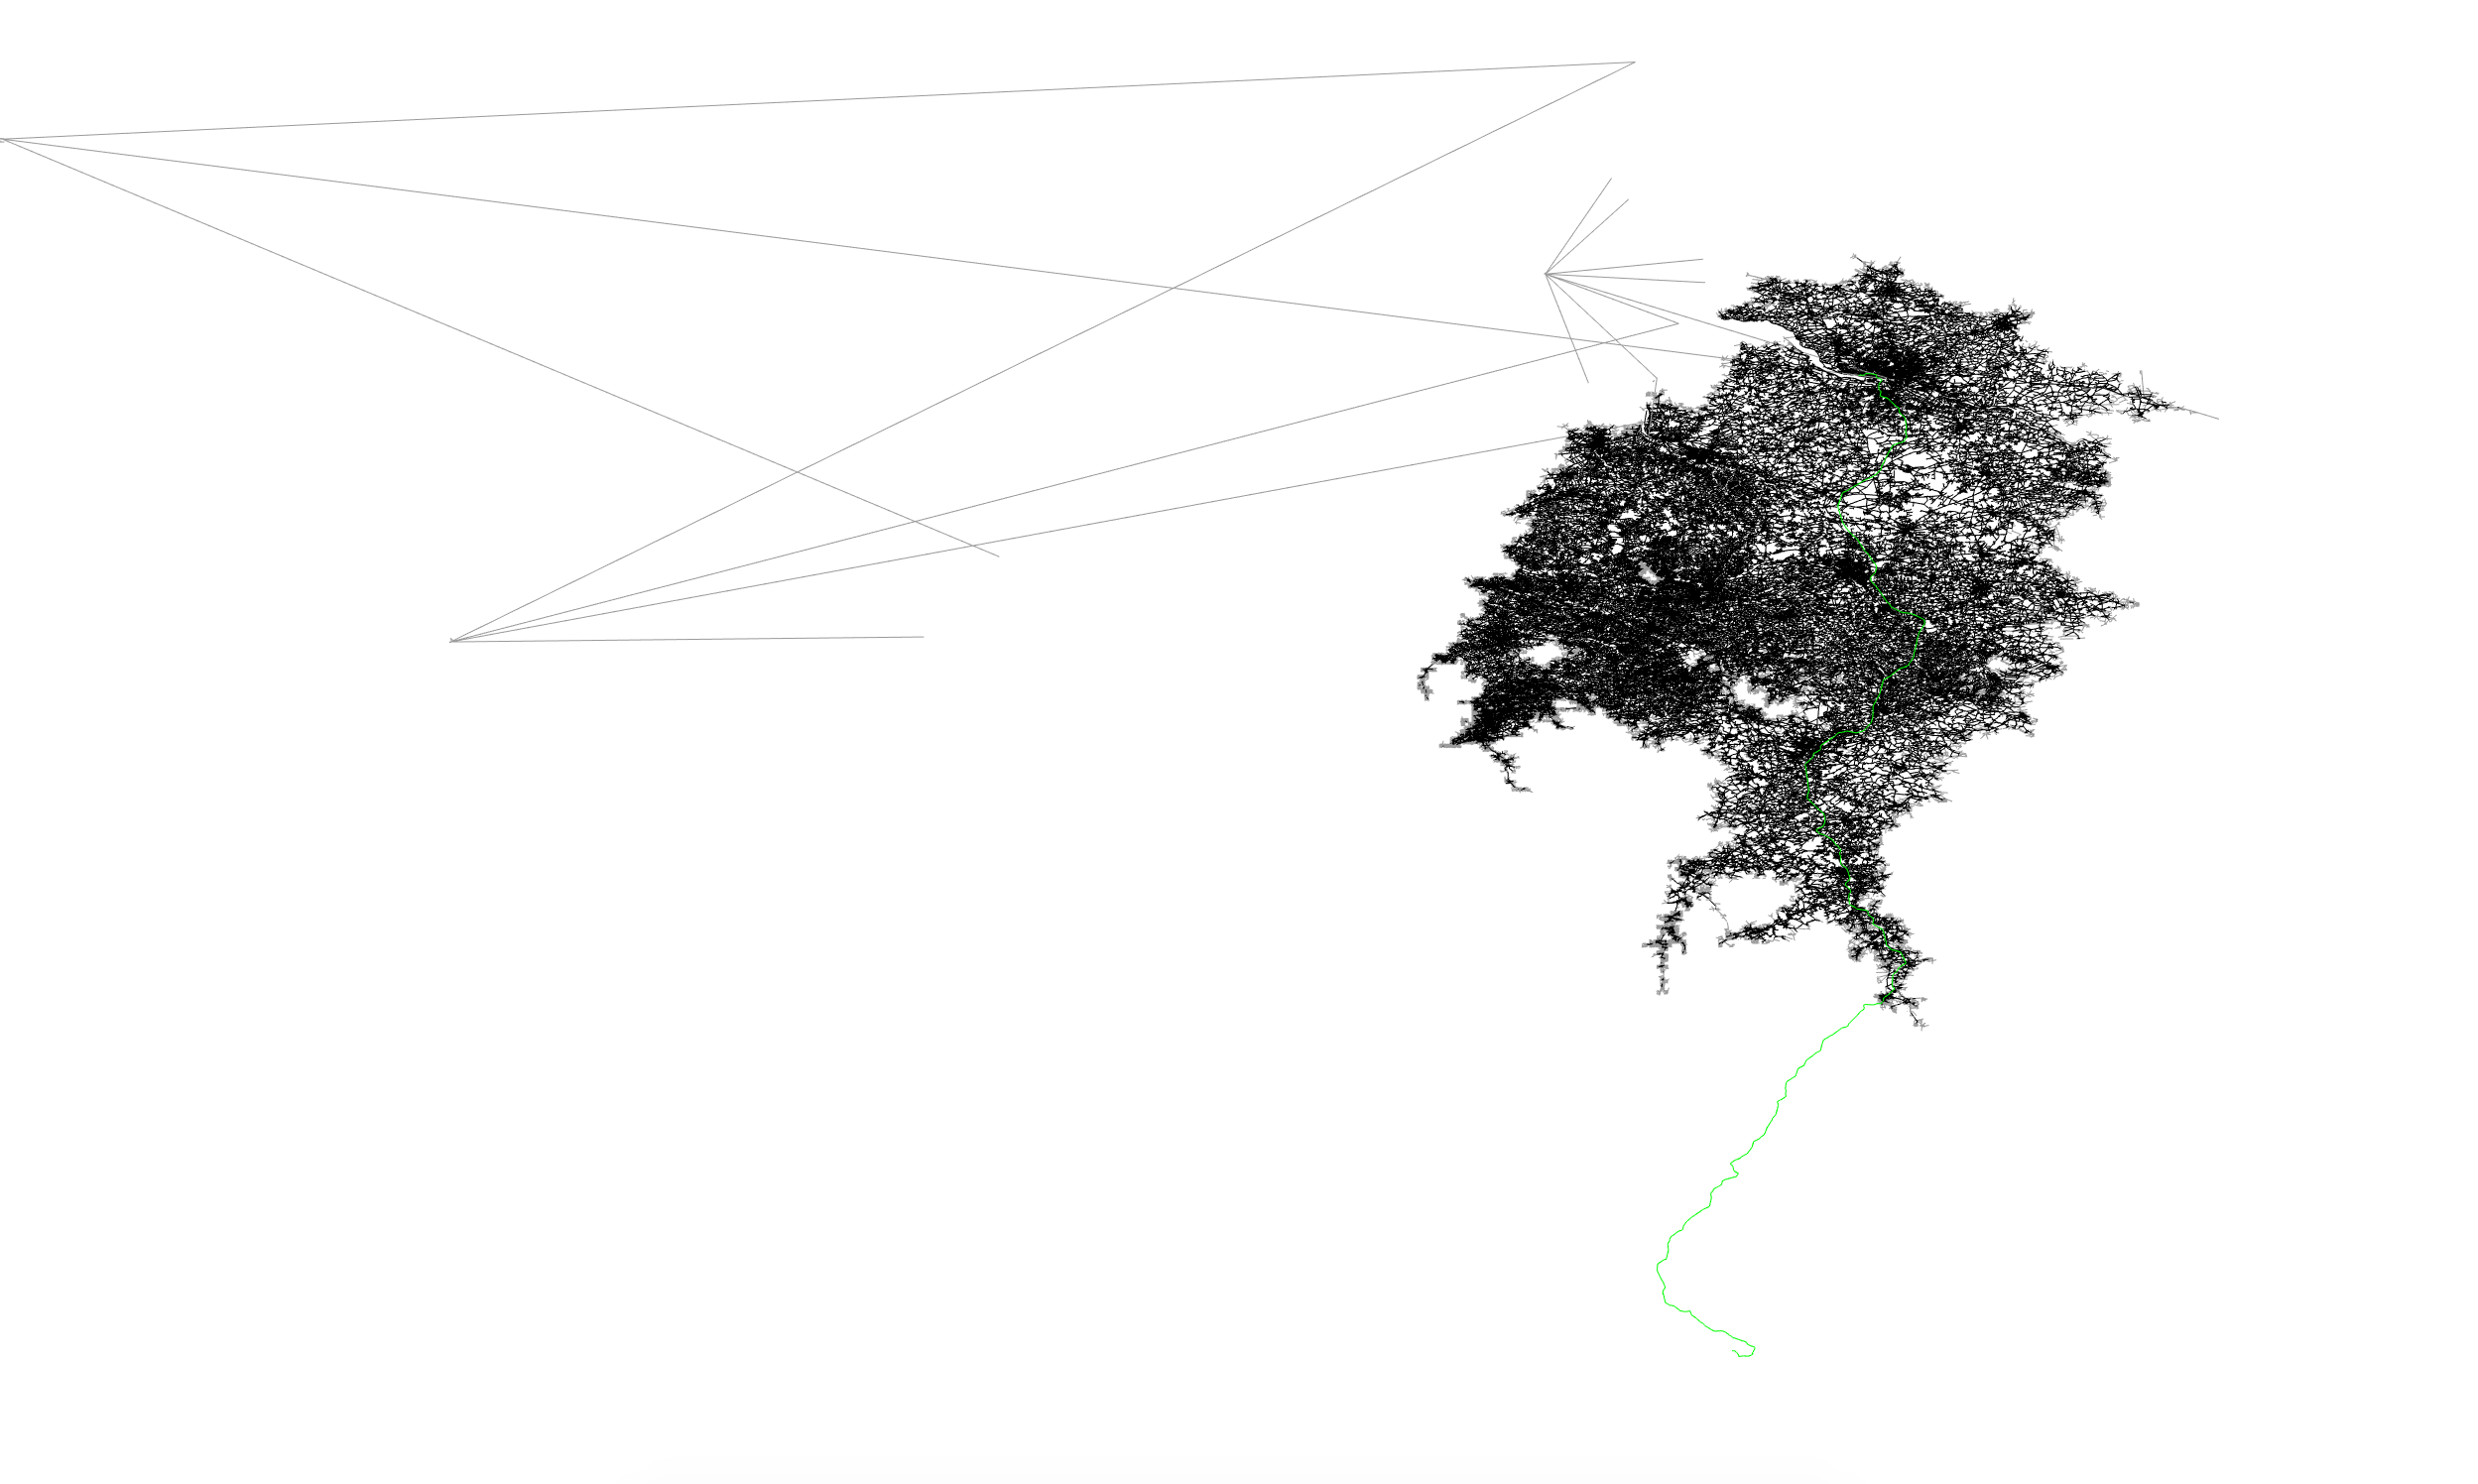
\includegraphics[width=0.5\textwidth]{Images/vis-tile-blocks-big.png}
\caption[]{Displaying all loaded edges. Those that has been passed by the algorithm in black and those that has only been loaded in grey.}
\label{fig:basic_tiles}
\end{figure}

As a result, we can see a basic tile structure in the visualization, which leads to a basic understanding about the loaded tiles during the algorithm.
However, as the algorithm evolves and the displayed graph grows tiles become much harder to distinguish from each other and especially in the inner graph it is not possible anymore to differentiate between different tiles.
On bigger graphs, as in \cref{fig:basic_tiles}, the tiles can not be distinguished from each other at all.
Therefore we want to add a new type of elements to the visualization, that will then represent the tiles.
Thanks to the decision to use the Equirectangular projection, mentioned in \cref{graph}, every tile is rectangular and has the same size.
Hence, it is possible to add rectangular shapes around the tiles without any bigger effort.

\begin{figure}[H]
    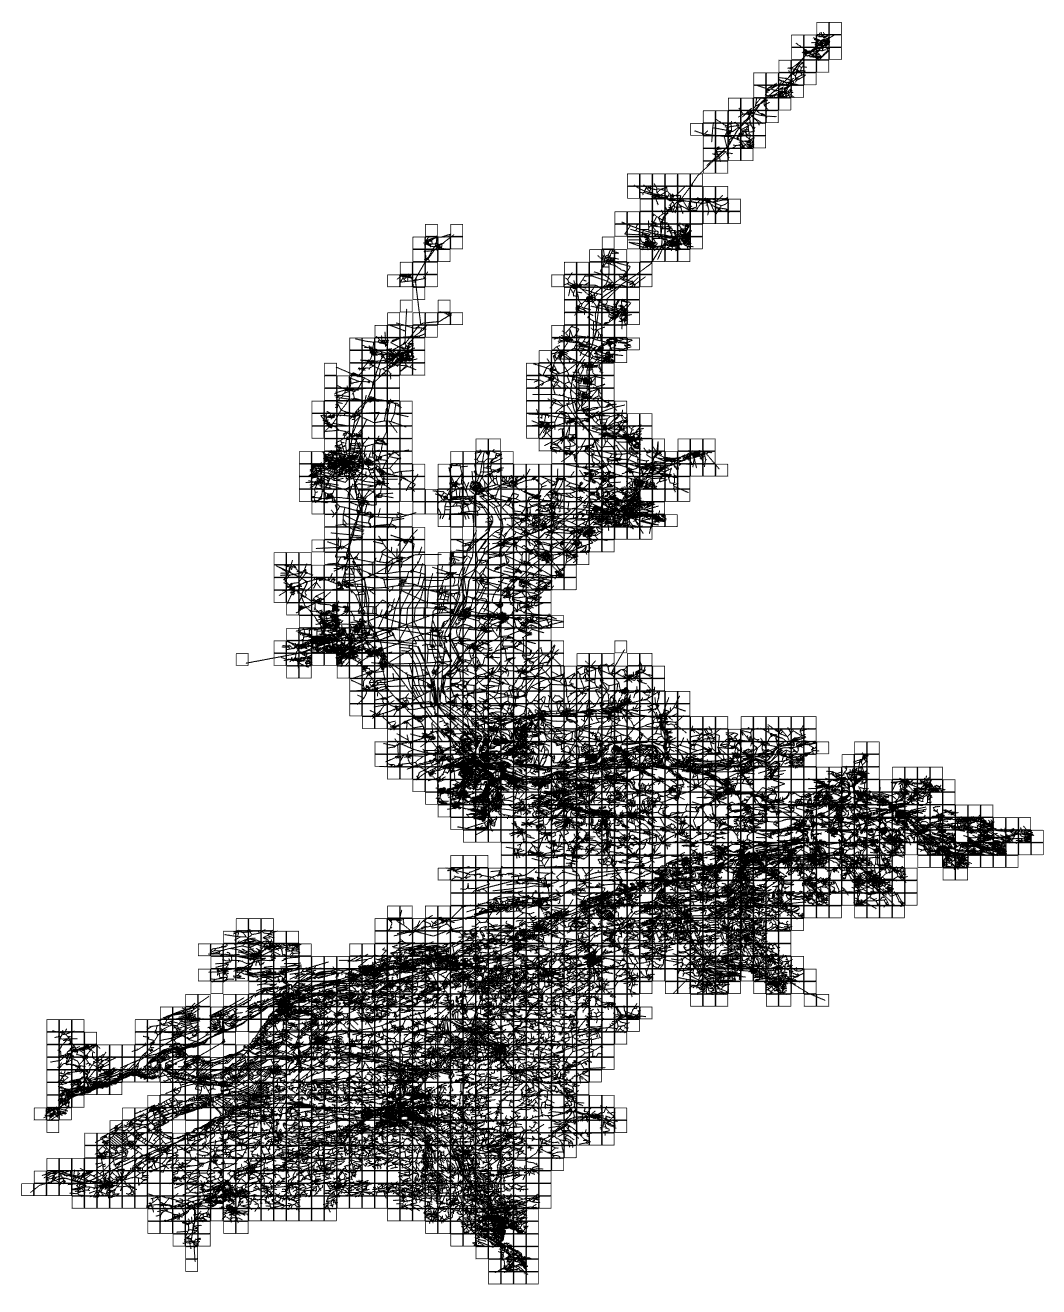
\includegraphics[width=\textwidth]{Images/vis-rectangular-tiles.png}
\caption[]{Representing tiles through rectangles.}
\label{fig:rectangle_tiles}
\end{figure}

As we can be seen in \cref{fig:rectangle_tiles} it is now possible to distinguish the tiles much better.
Furthermore, the rectangles became the most important source of information on a bigger routes as the biggest part of the edges is not recognizable individually and they even became obstructive for the comprehensibility.
The biggest value added by the edges on this level is the information about the current step of the algorithm which becomes difficult to recognize on bigger graphs as  well.
As we want to change this, we will transfer this information to a higher level and therefore color the tile the algorithm is currently processing.
As a result, we can now stop displaying the edges which makes the visualization much more uncluttered and leads to a major performance boost.

\begin{figure}[H]
    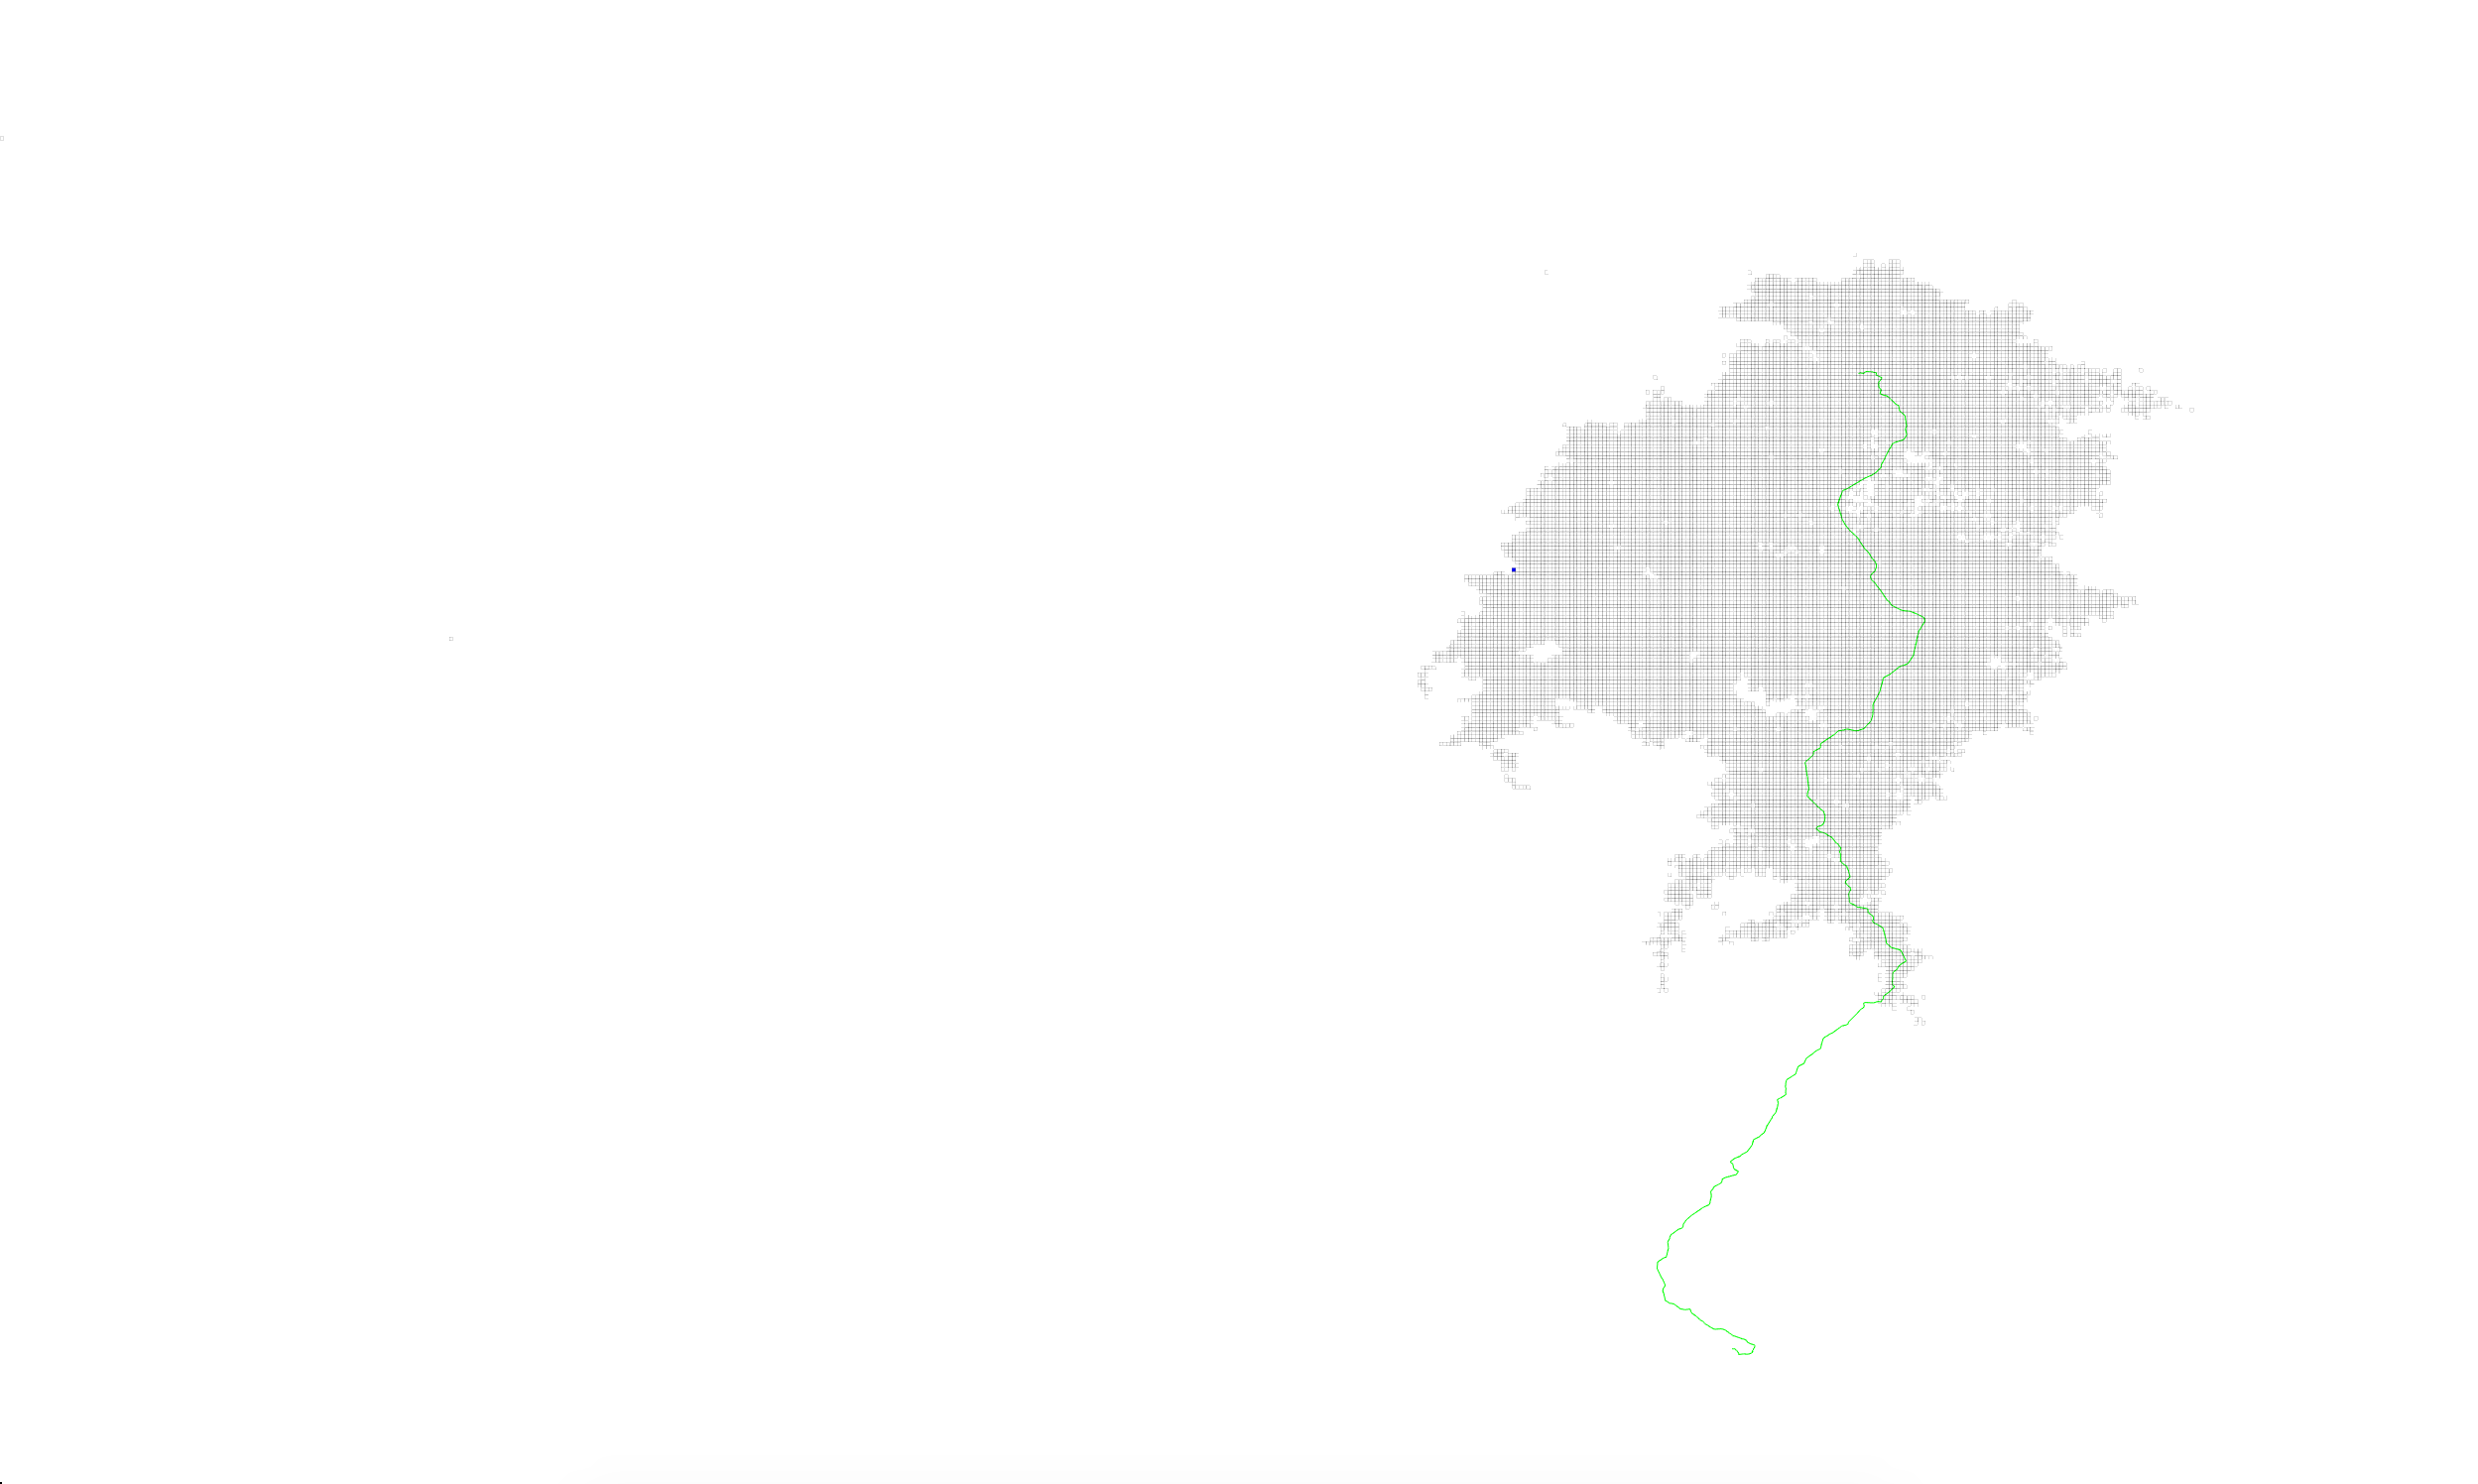
\includegraphics[width=\textwidth]{Images/vis-current-tile.png}
\caption[]{Representing tiles through rectangles.}
\label{fig:color_current_tile}
\end{figure}


In \cref{fig:color_current_tile}, we see that we got an abstract visualization now, that visualizes the algorithms using rectangles.
Even though this visualization is clean for bigger routes, understanding the actual behavior of the algorithms is still hard, as a single tile is only colored for milliseconds when accessed and therefore it is hard to see the loading of tiles in a larger context.
Hence, we want to try to fix this by introducing a method, we will call aging of tiles.
This means that the currently processed tile is still colored, but different than in the approach before, we do not uncolor it immediately, but over time.
Therefore the tile becomes a bit brighter every step of the algorithm.

\begin{figure}[H]
    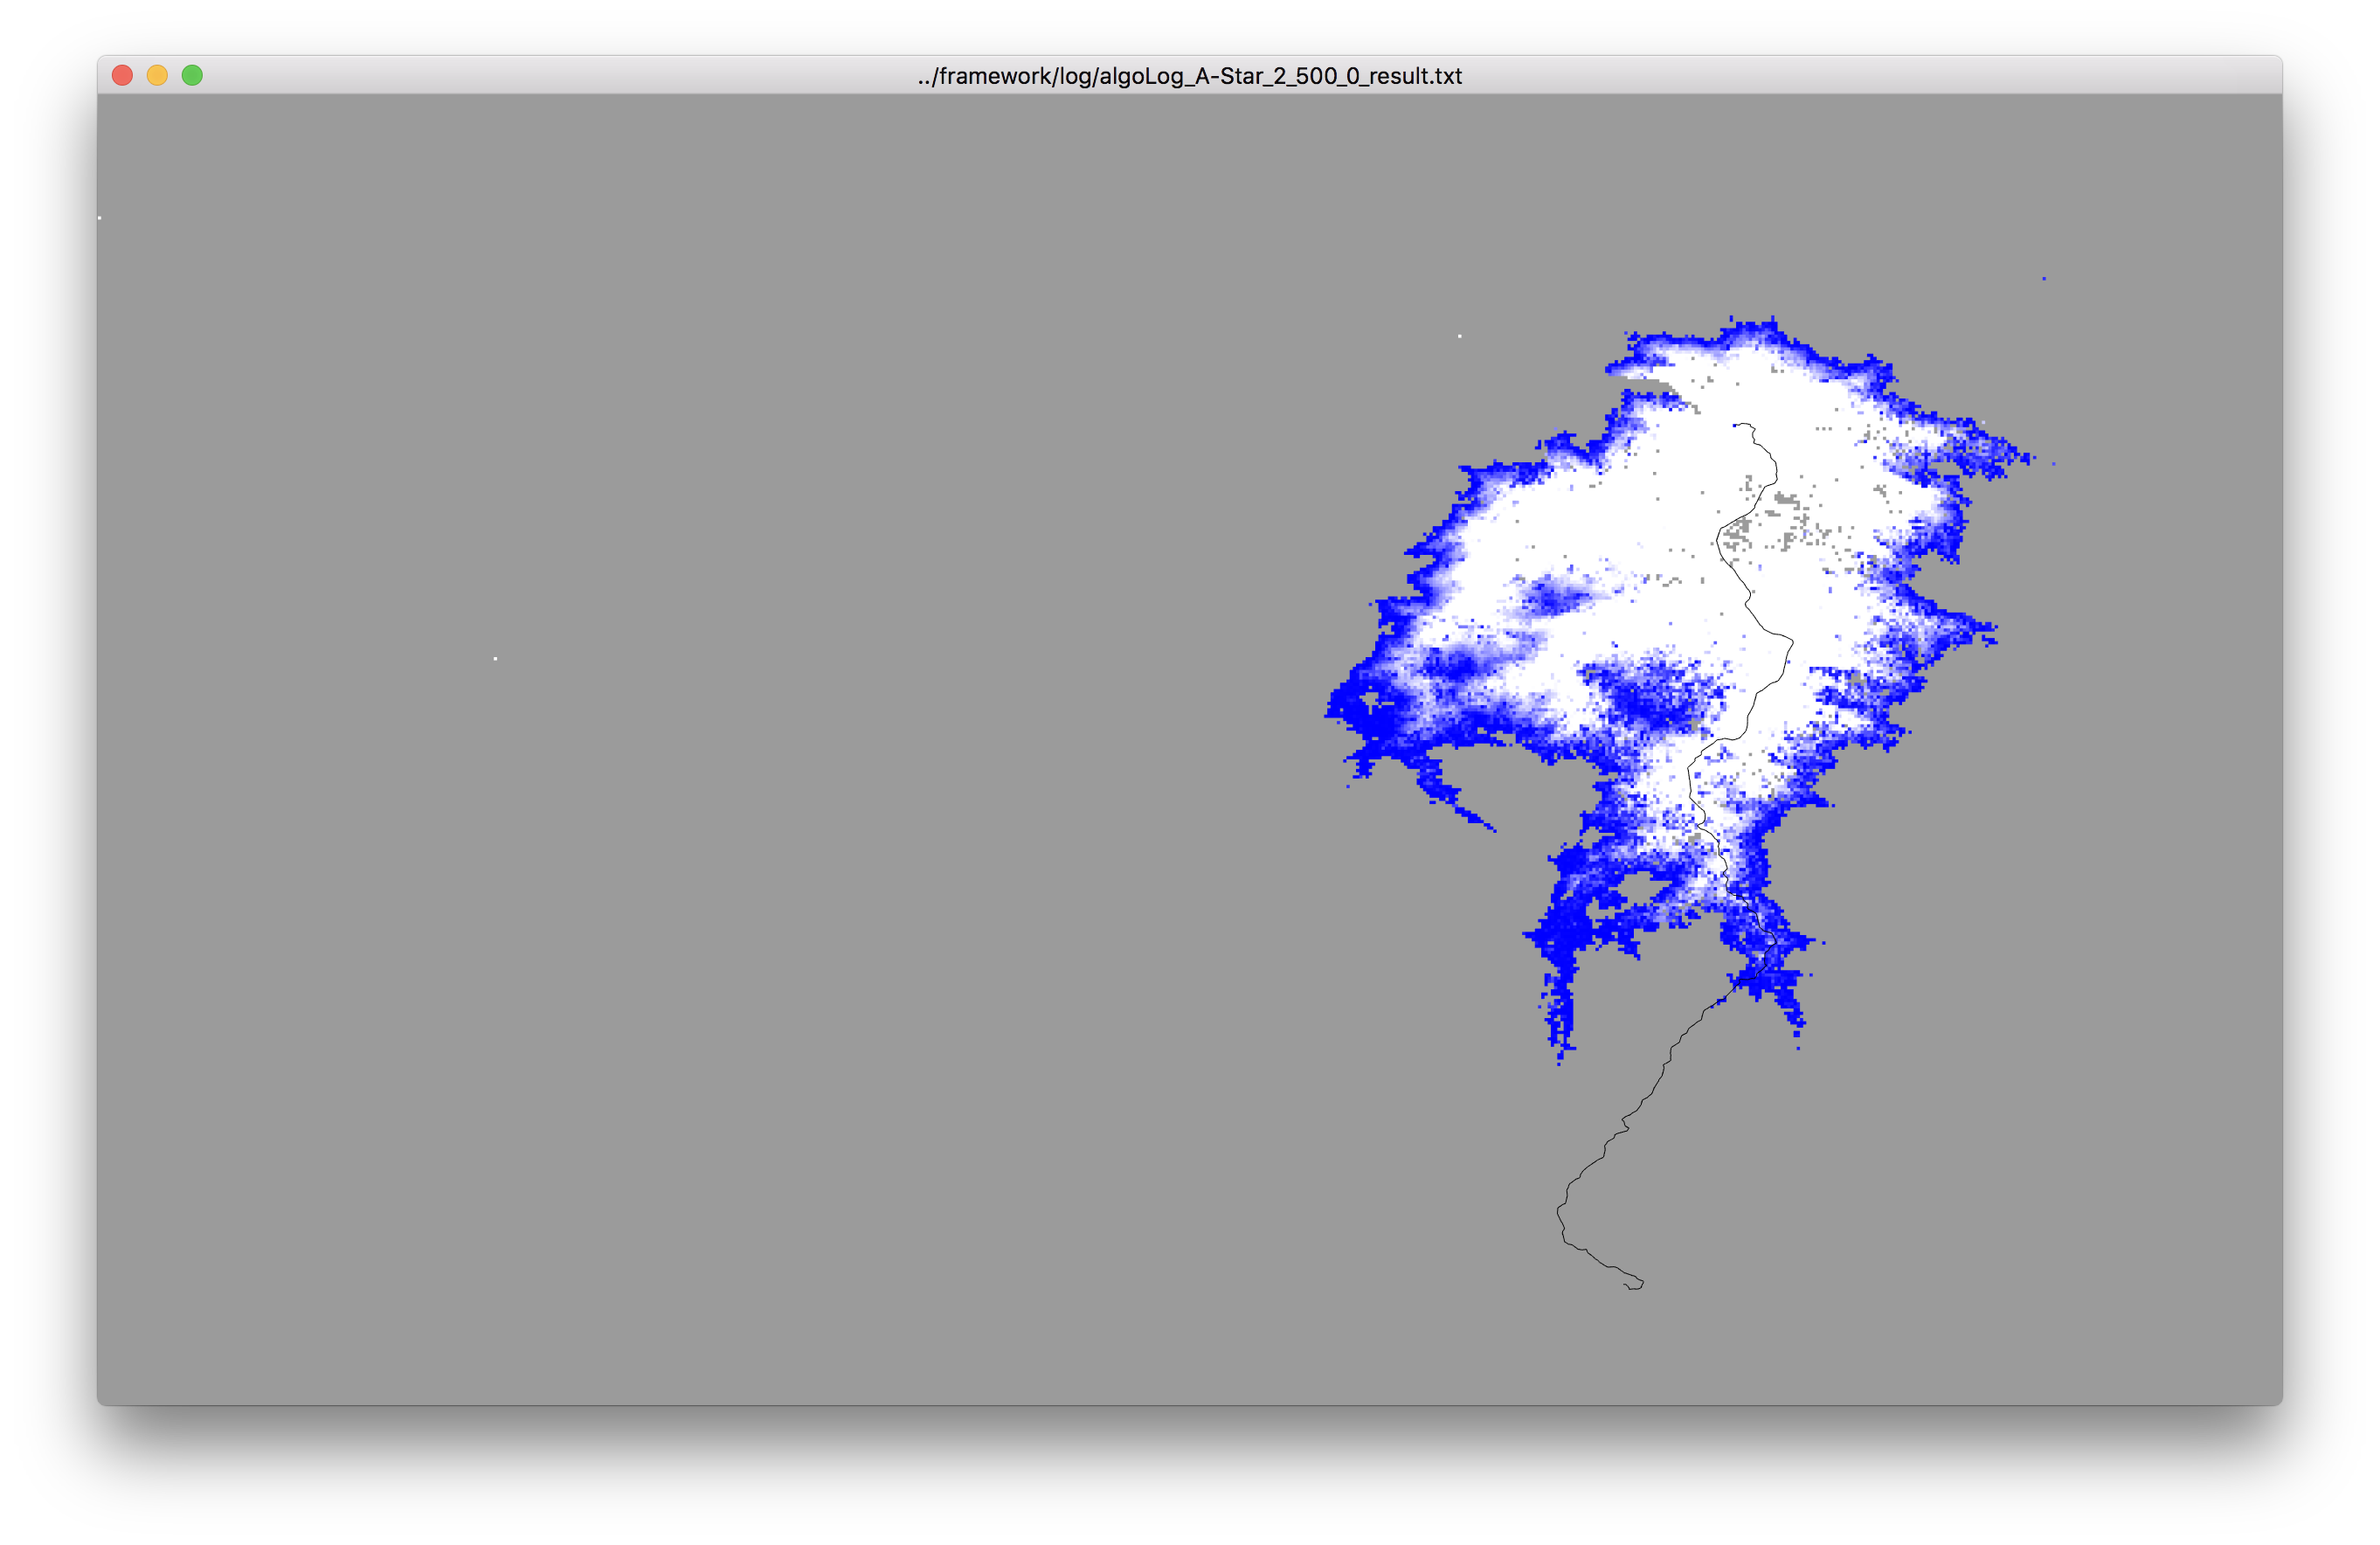
\includegraphics[width=\textwidth]{Images/vis-aged-coloring.png}
\caption[]{Age based coloring. Newly loaded tiles are colored blue and get brighter the longer they have not been loaded.}
\label{fig:color_aged_tile}
\end{figure}

In \cref{fig:color_aged_tile} we see that this approach leads to a much better understanding of the sequence of tile-loads.
Thereby it leads to a much better comprehensibility of how the algorithm performs on the underlying graph and the specific route.
In \cref{fig:color_aged_tile} for example, we can see that most of the recently loaded tiles are located on the outside of the explored graph, but there are three bigger parts in the inner part which should maybe be examined more specific.


\subsection{Visualizing the Cache}

Based on what we build in \cref{tiles} we can now start thinking about the cache.
In \cref{specification} we already mentioned, that the accessing of a tile itself is not the expensive operation for the algorithm, but loading a tile into the cache.
Therefore we should definitely include the cache into the visualization somehow.
Because we already introduced the tiled visualization in \cref{tiles}, we have a good foundation to work with.
As a first approach, we will color all the tiles that are currently stored in the cache and therefore accessible for the algorithm without extra costs.

\begin{figure}[H]
    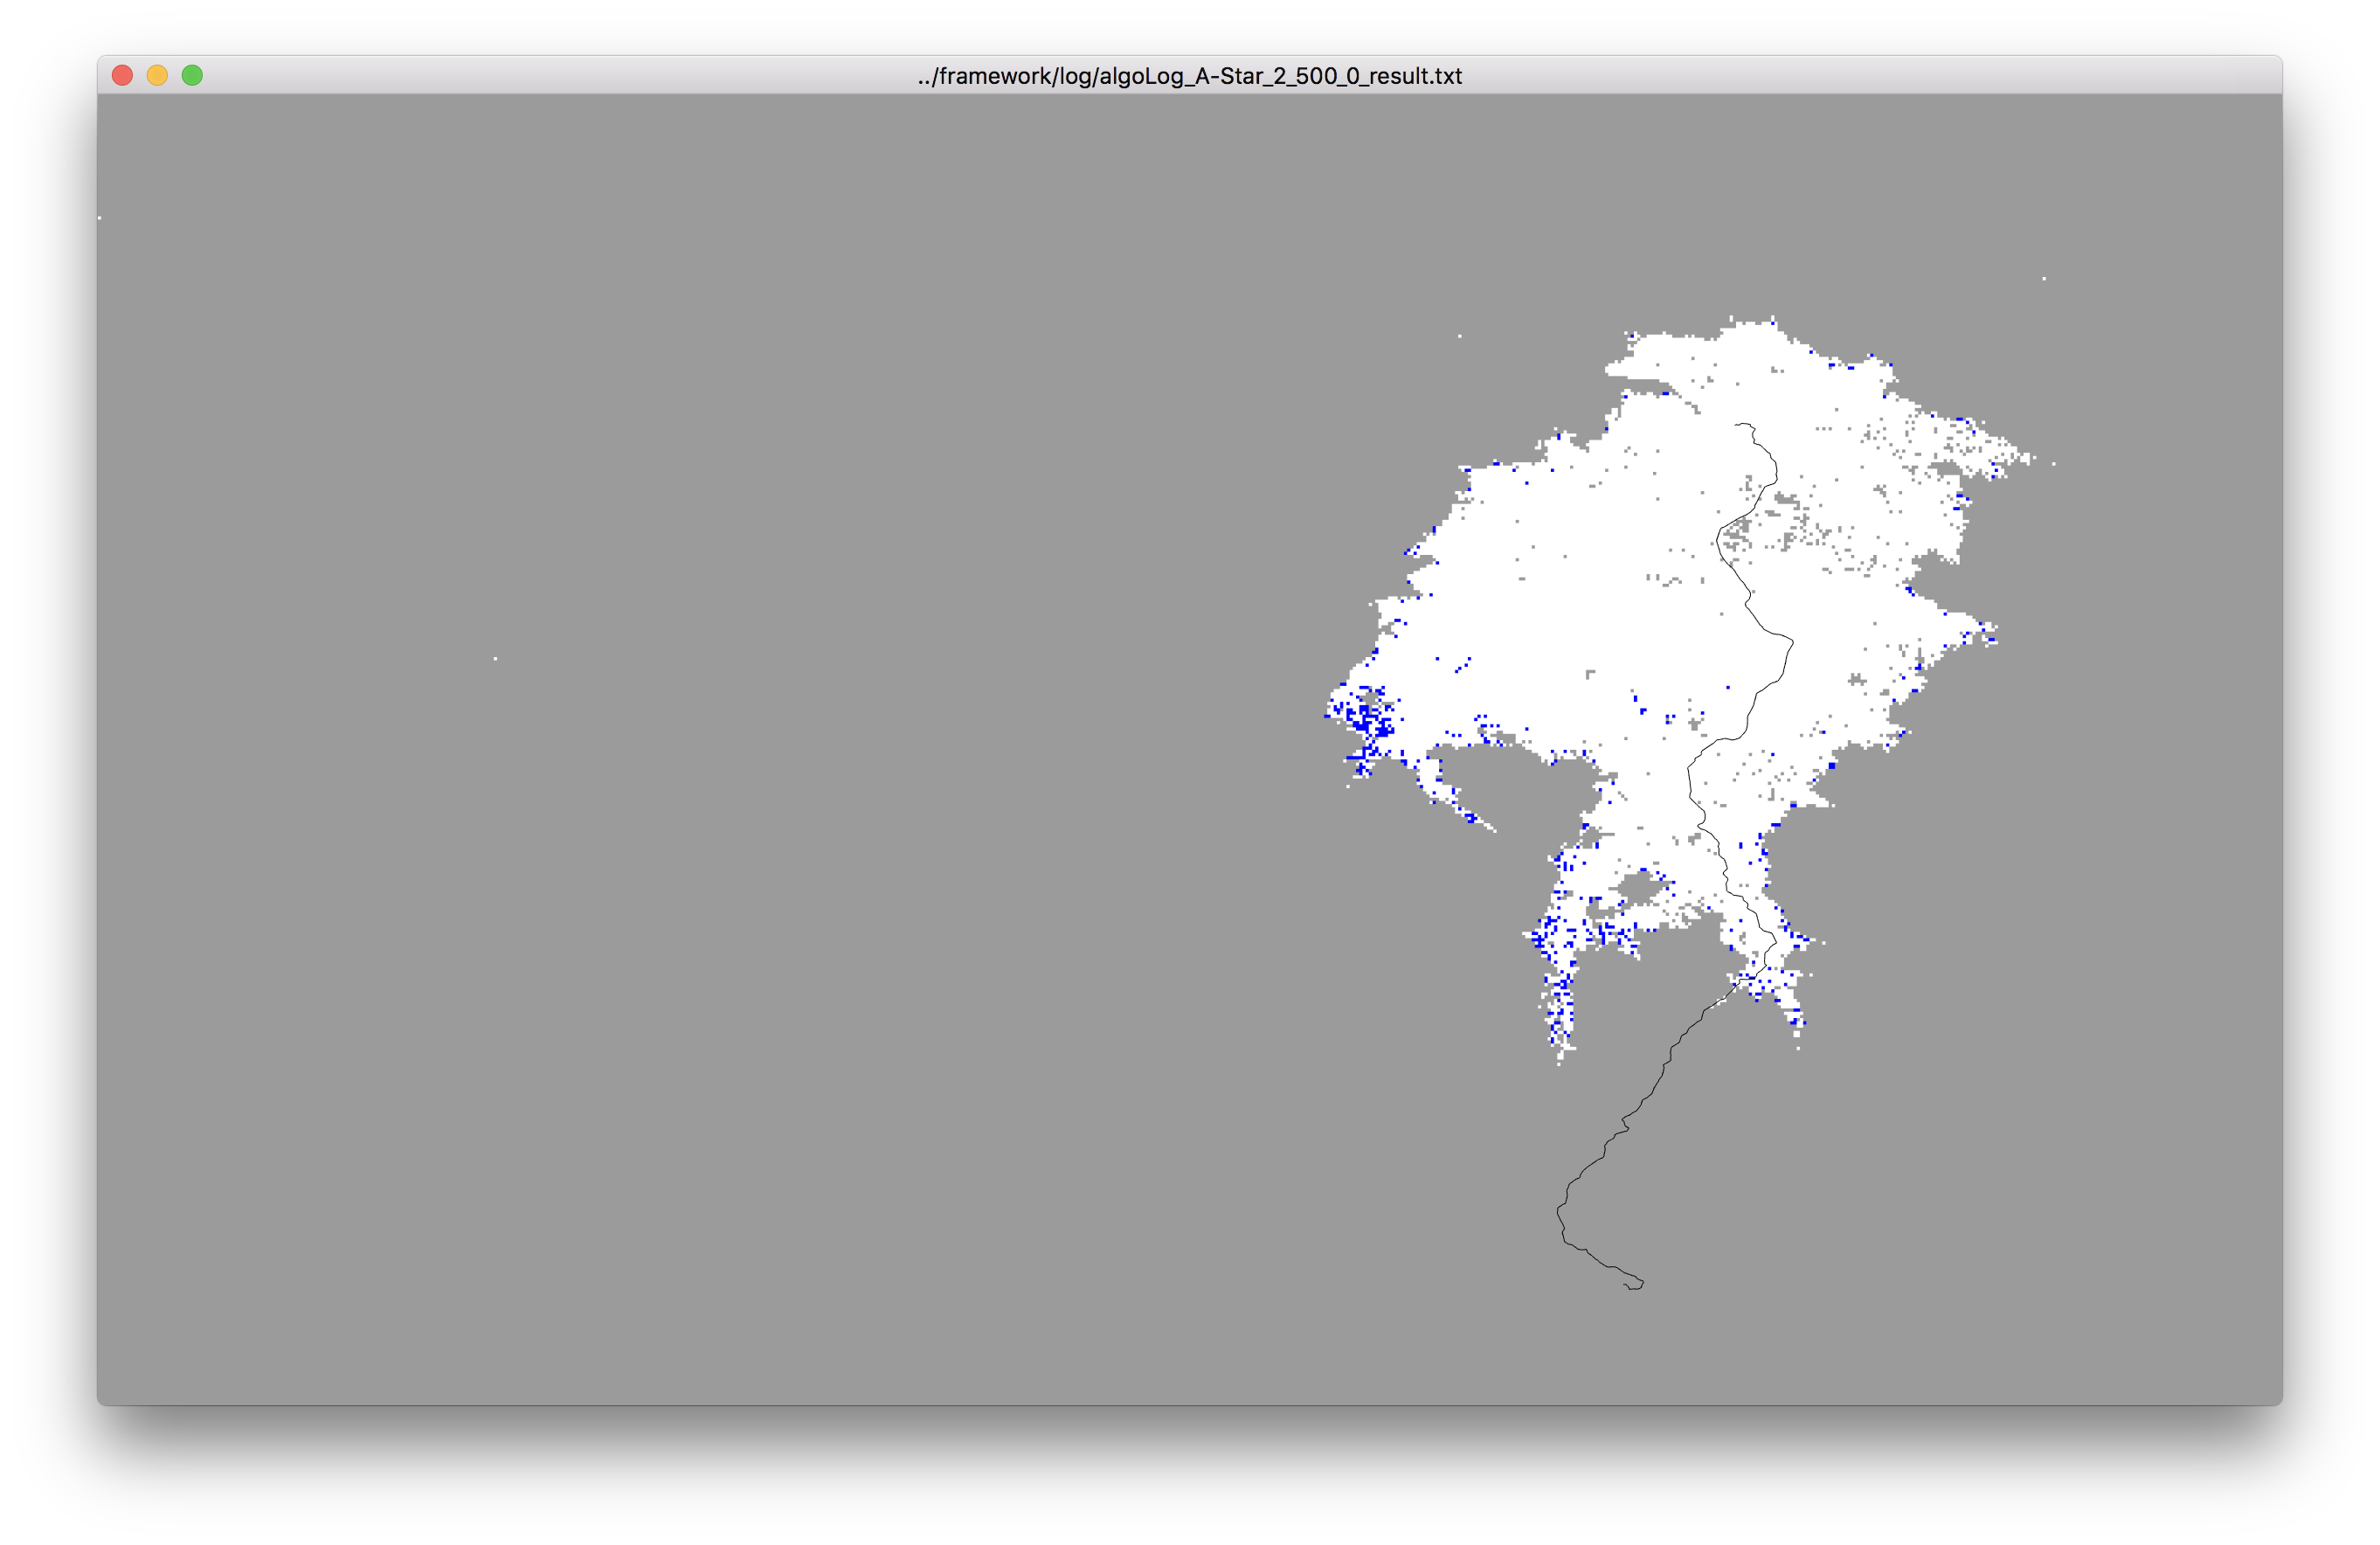
\includegraphics[width=\textwidth]{Images/vis-basic-cache.png}
\caption[]{Representing the cache. The cache is represented by the blue rectangular shapes.}
\label{fig:cache_coloring}
\end{figure}

In \cref{fig:cache_coloring} we can see, that we did not color the tiles based on their age anymore.
Due to the colored cache, we achieved an improved understanding of past loaded tiles and the aged based coloring would furthermore distract from the important cache.

At this point, it would be good to see how often a tile was loaded in the cache, at any point of the visualization, without knowing what happened before.
Therefore, we now want to color all the tiles, except those that are in the cache, according to the frequency they have been loaded.
As red is often associated with negative occurrences we will now color a tile a little redder every time it was loaded into the cache.

\begin{figure}[H]
    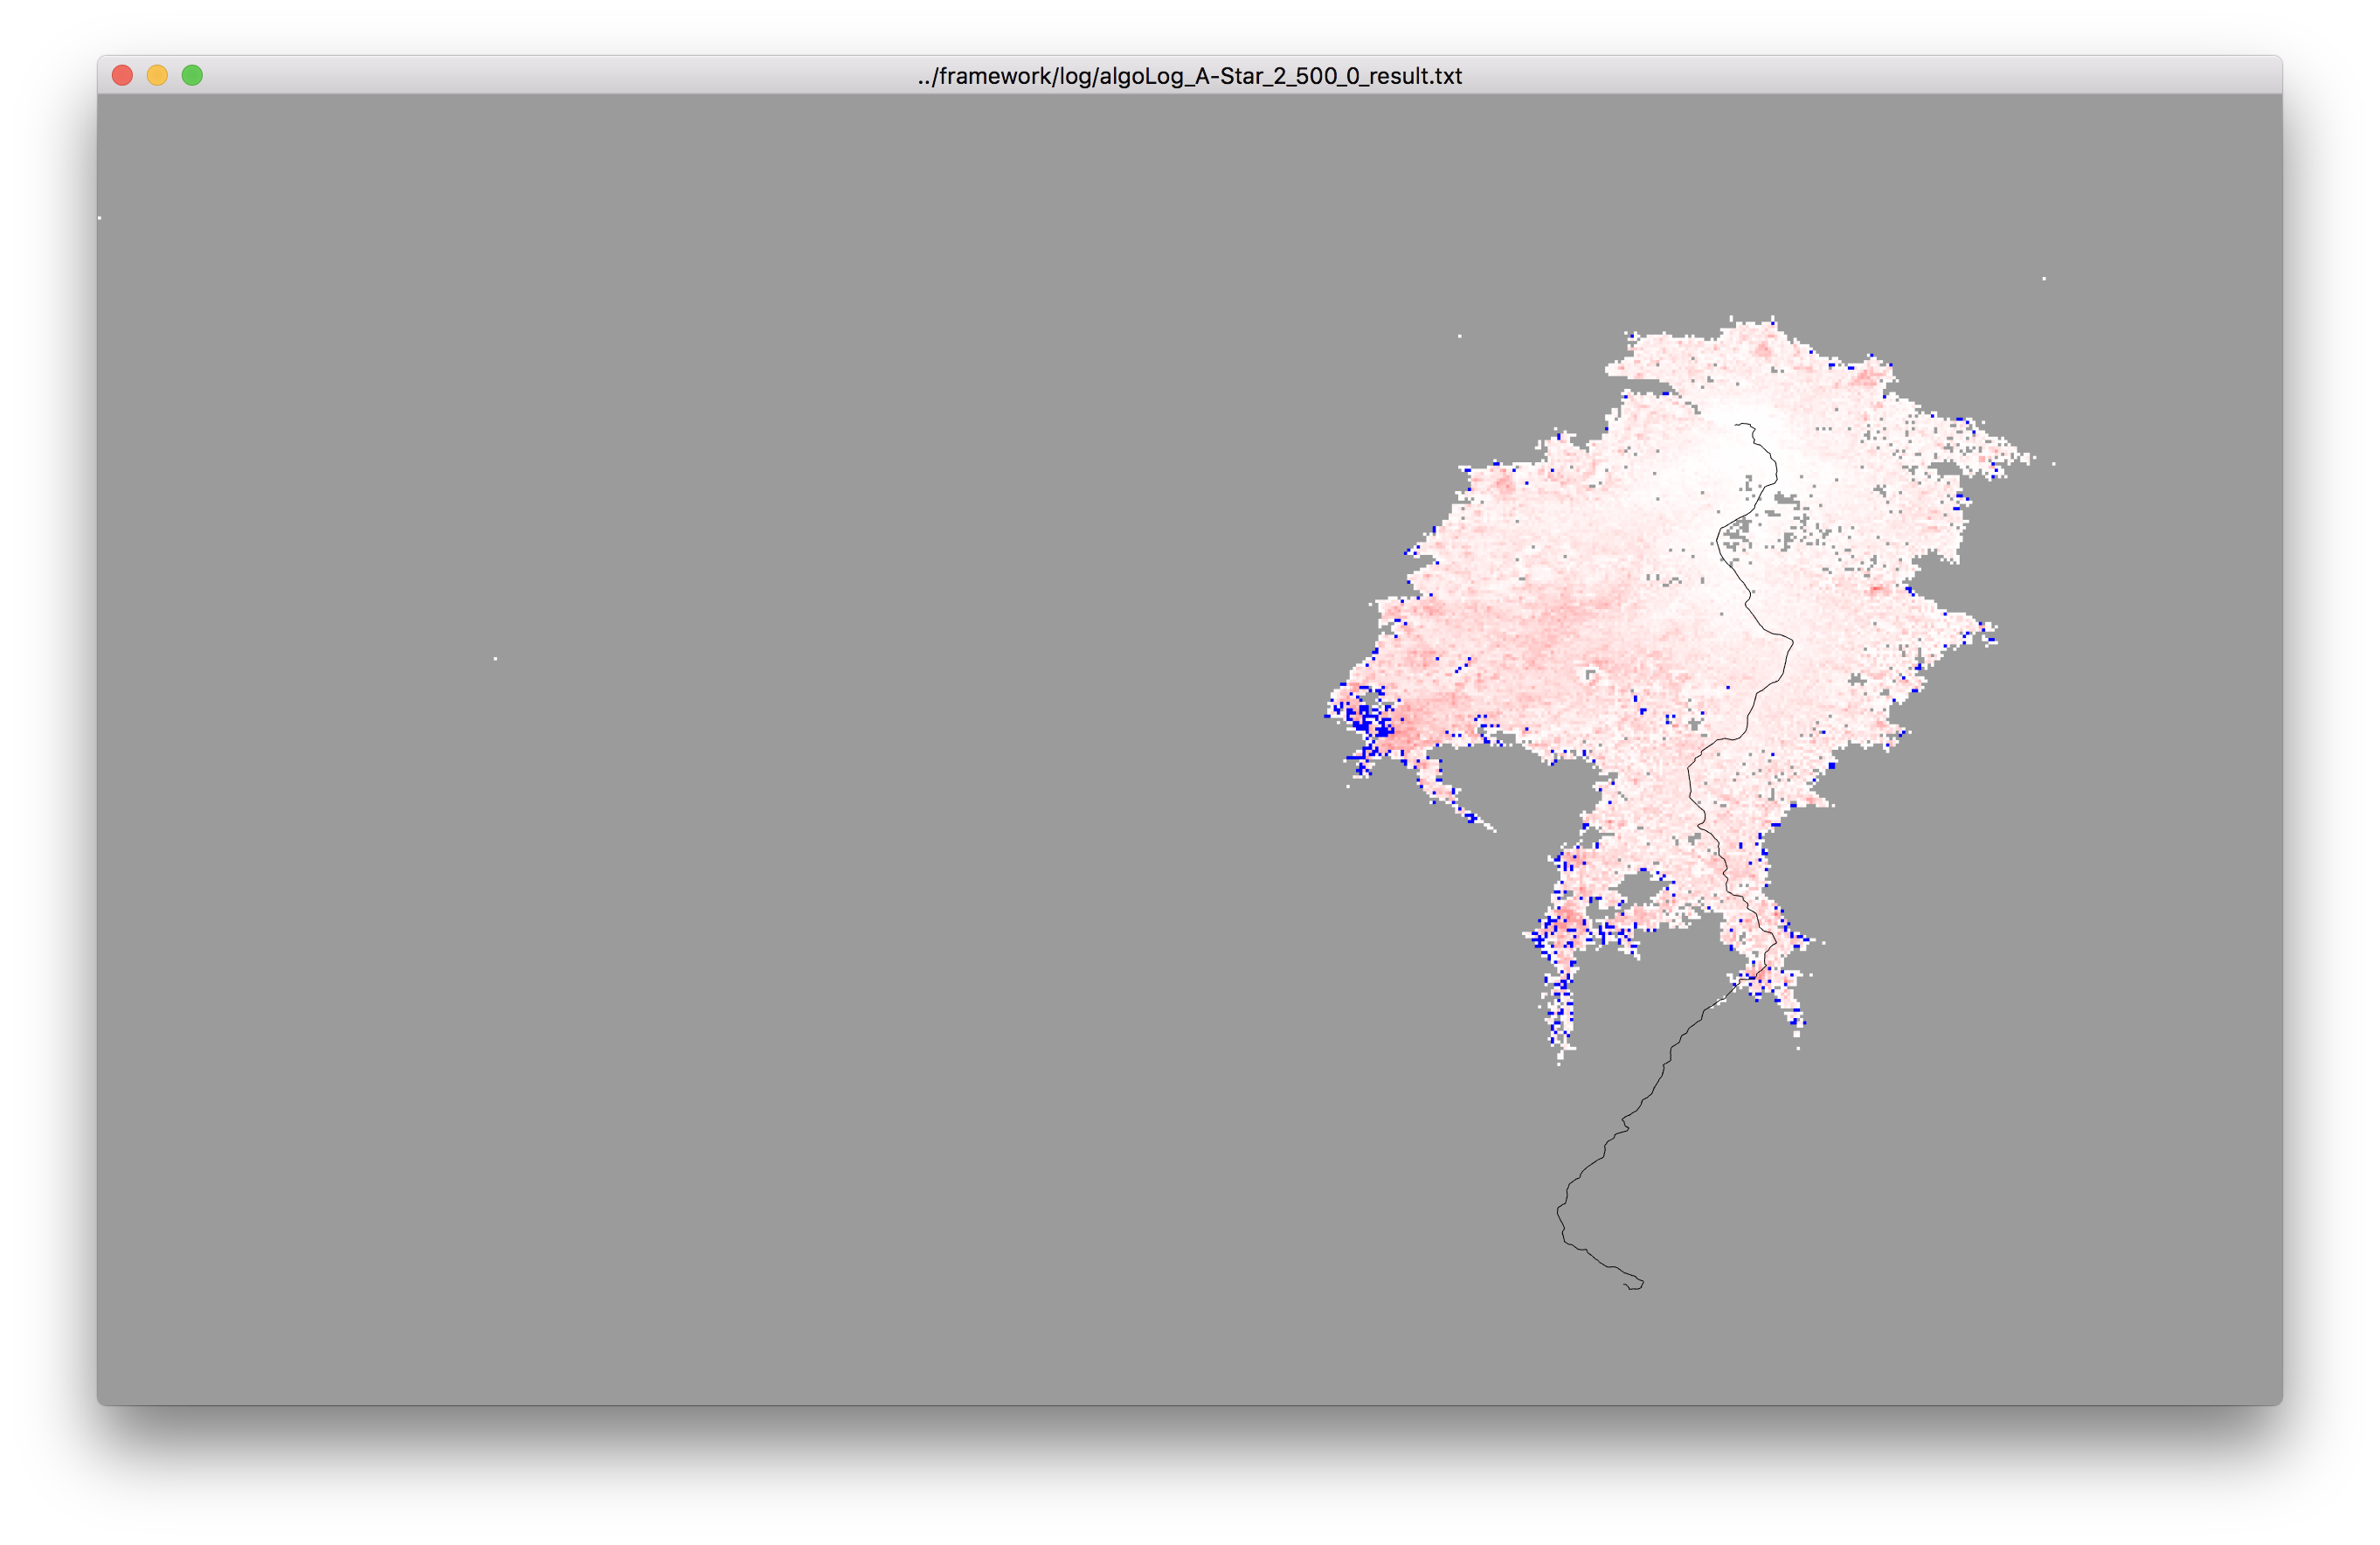
\includegraphics[width=\textwidth]{Images/vis-rgb-cache.png}
\caption[]{Coloring the tiles according to the amount of reloads. Red tiles has been loaded more often.}
\label{fig:reload_coloring_white}
\end{figure}

By coloring the reloads this way, we can now see how good our algorithm performs and in which regions more reloads occur.
With this color scheme bigger differences in tile loading can be distinguished from each other easily.
Nevertheless smaller differences are hard to recognize.
Therefore, we want to try another color scale.
By setting the color of once loaded tiles to green and turn it into red the more the tile was loaded we hope to achieve a bigger and clearer contrast between slightly different tile loads.
In addition, green fits great to the association of red, as it is often used as an antagonist of red and is often associated with positive occurrences.

\begin{figure}[H]
    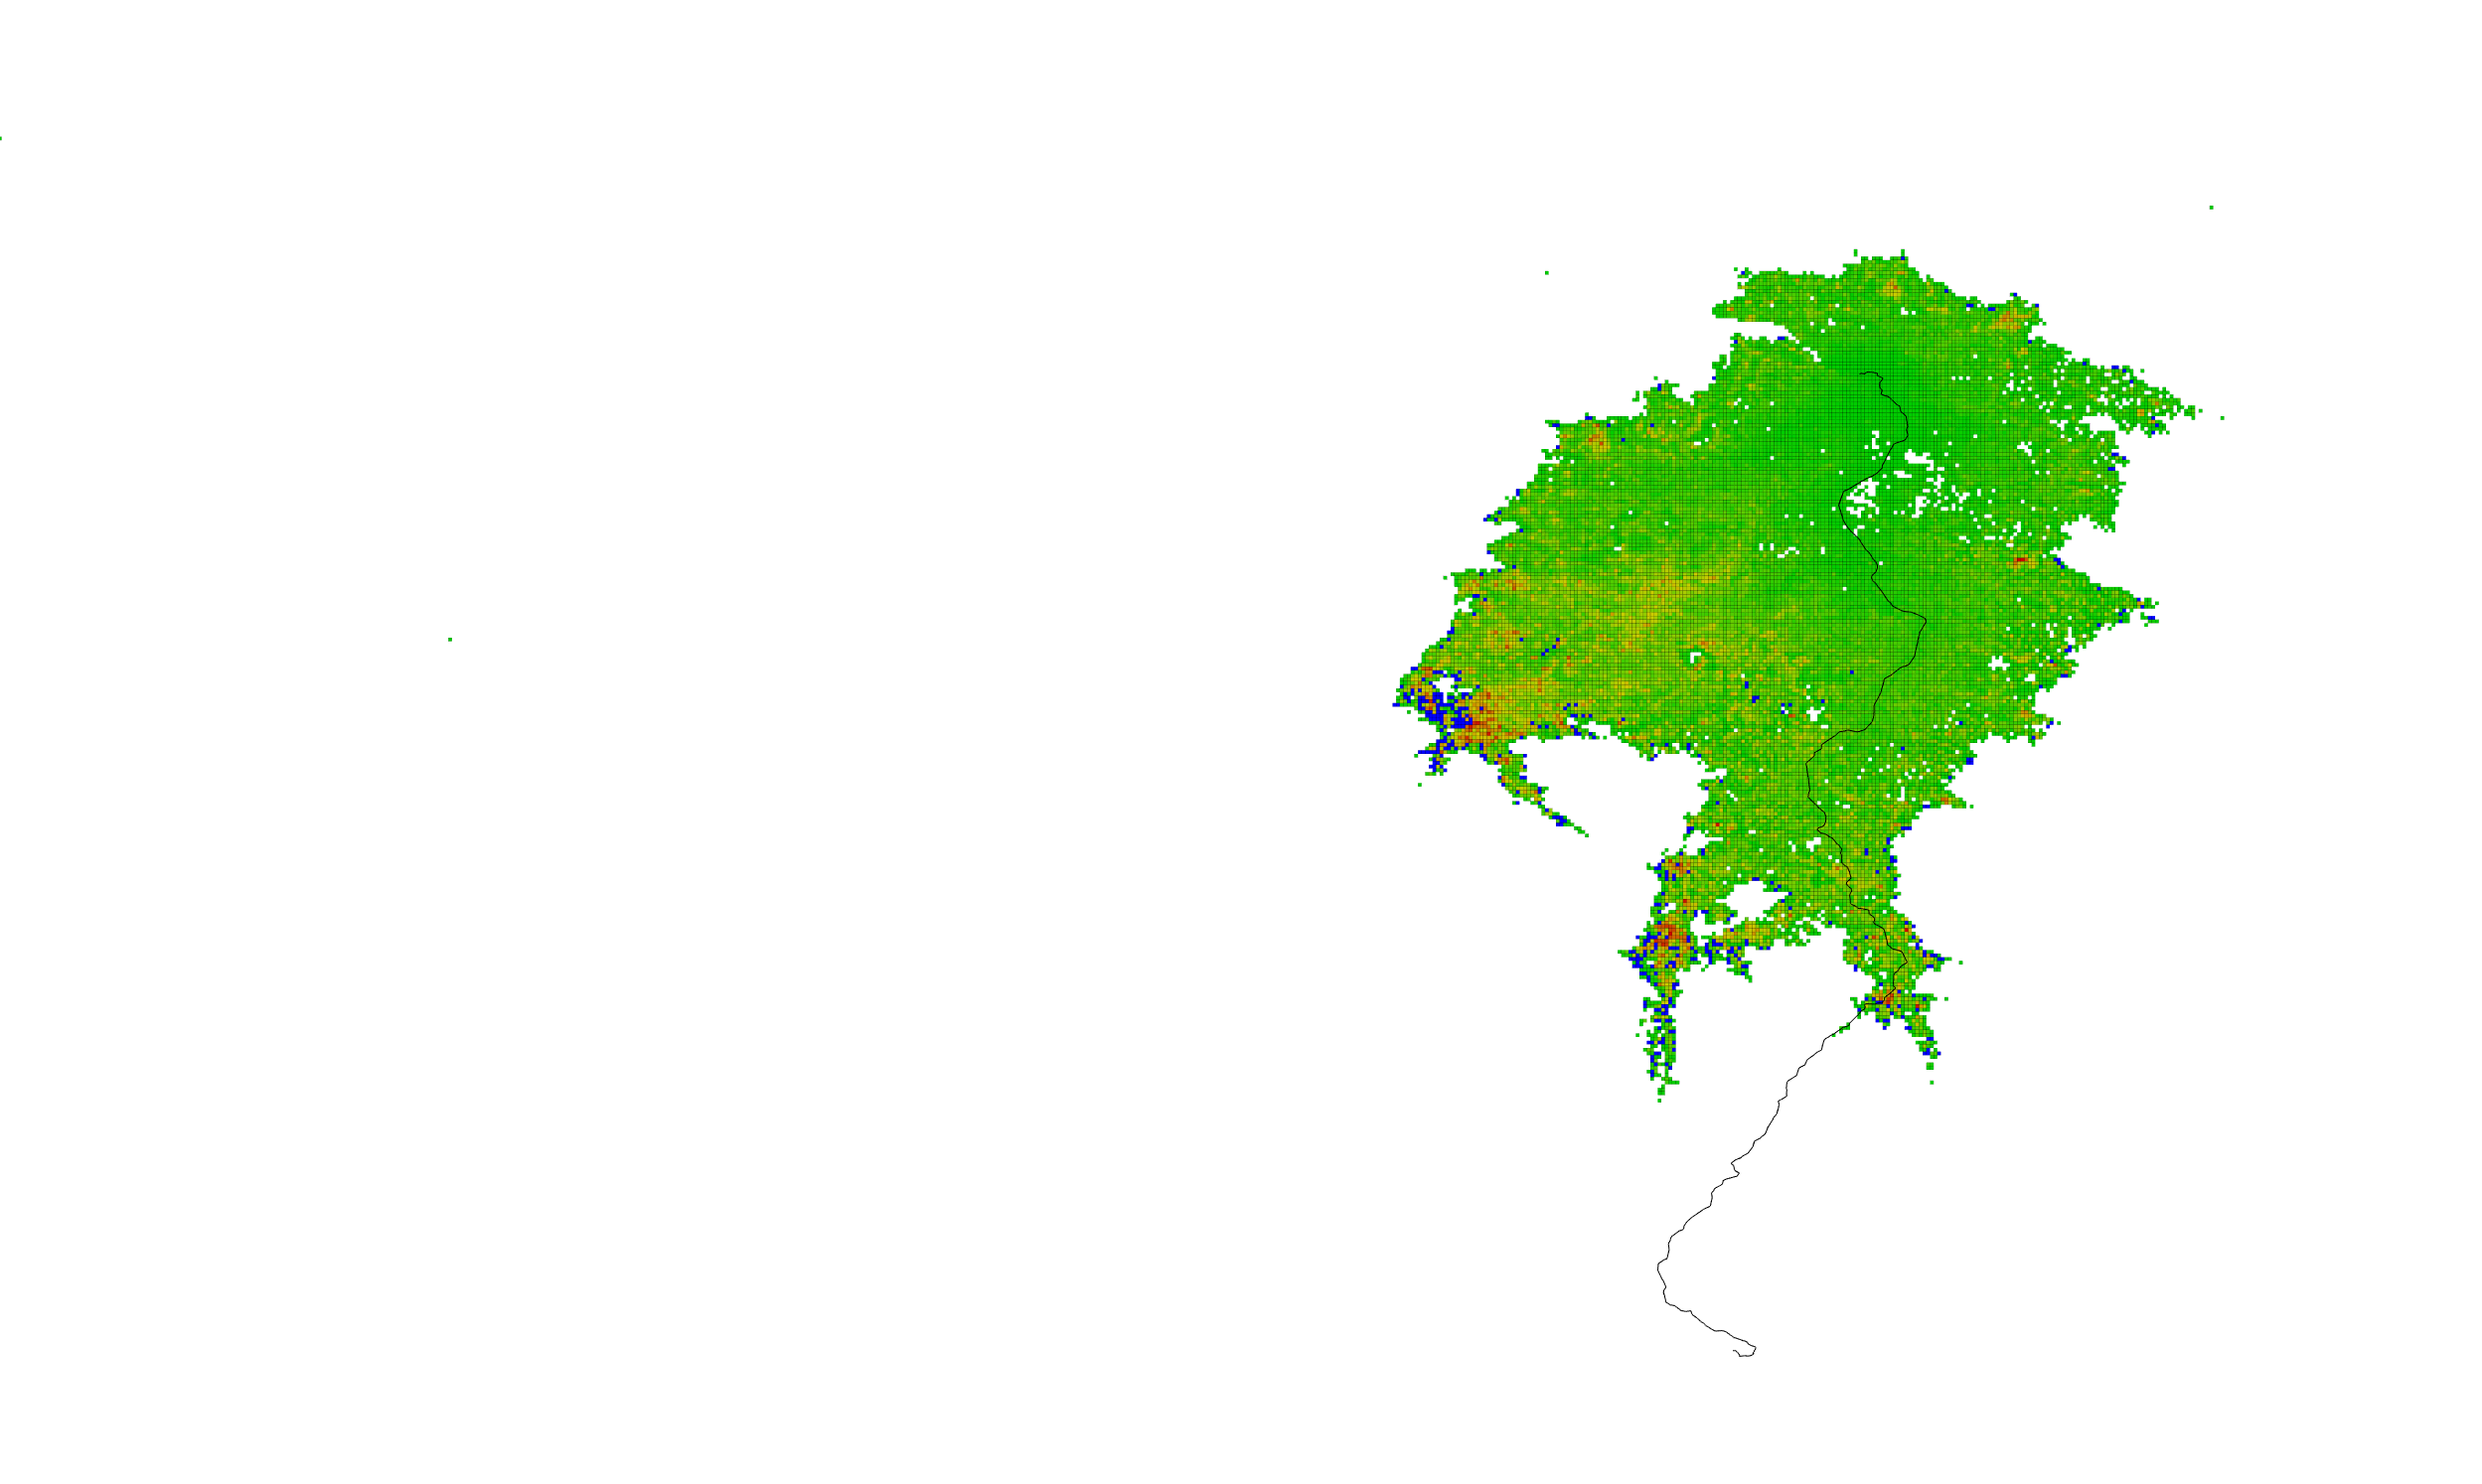
\includegraphics[width=\textwidth]{Images/vis-hsv-cache.png}
\caption[]{Changed color scheme. Now the tiles change their color from green to red.}
\label{fig:reload_coloring_hsv}
\end{figure}

In \cref{fig:reload_coloring_hsv} we see the differences between two similar values a little better now.
In addition, the graph distinguished from the background much better now and the visualization looks much better.

\section{Compare algorithms}

After having developed multiple algorithms, comparing different algorithms becomes more important.
Therefore we could simply start two visualizations and display them next to each other.

\begin{figure}[H]
    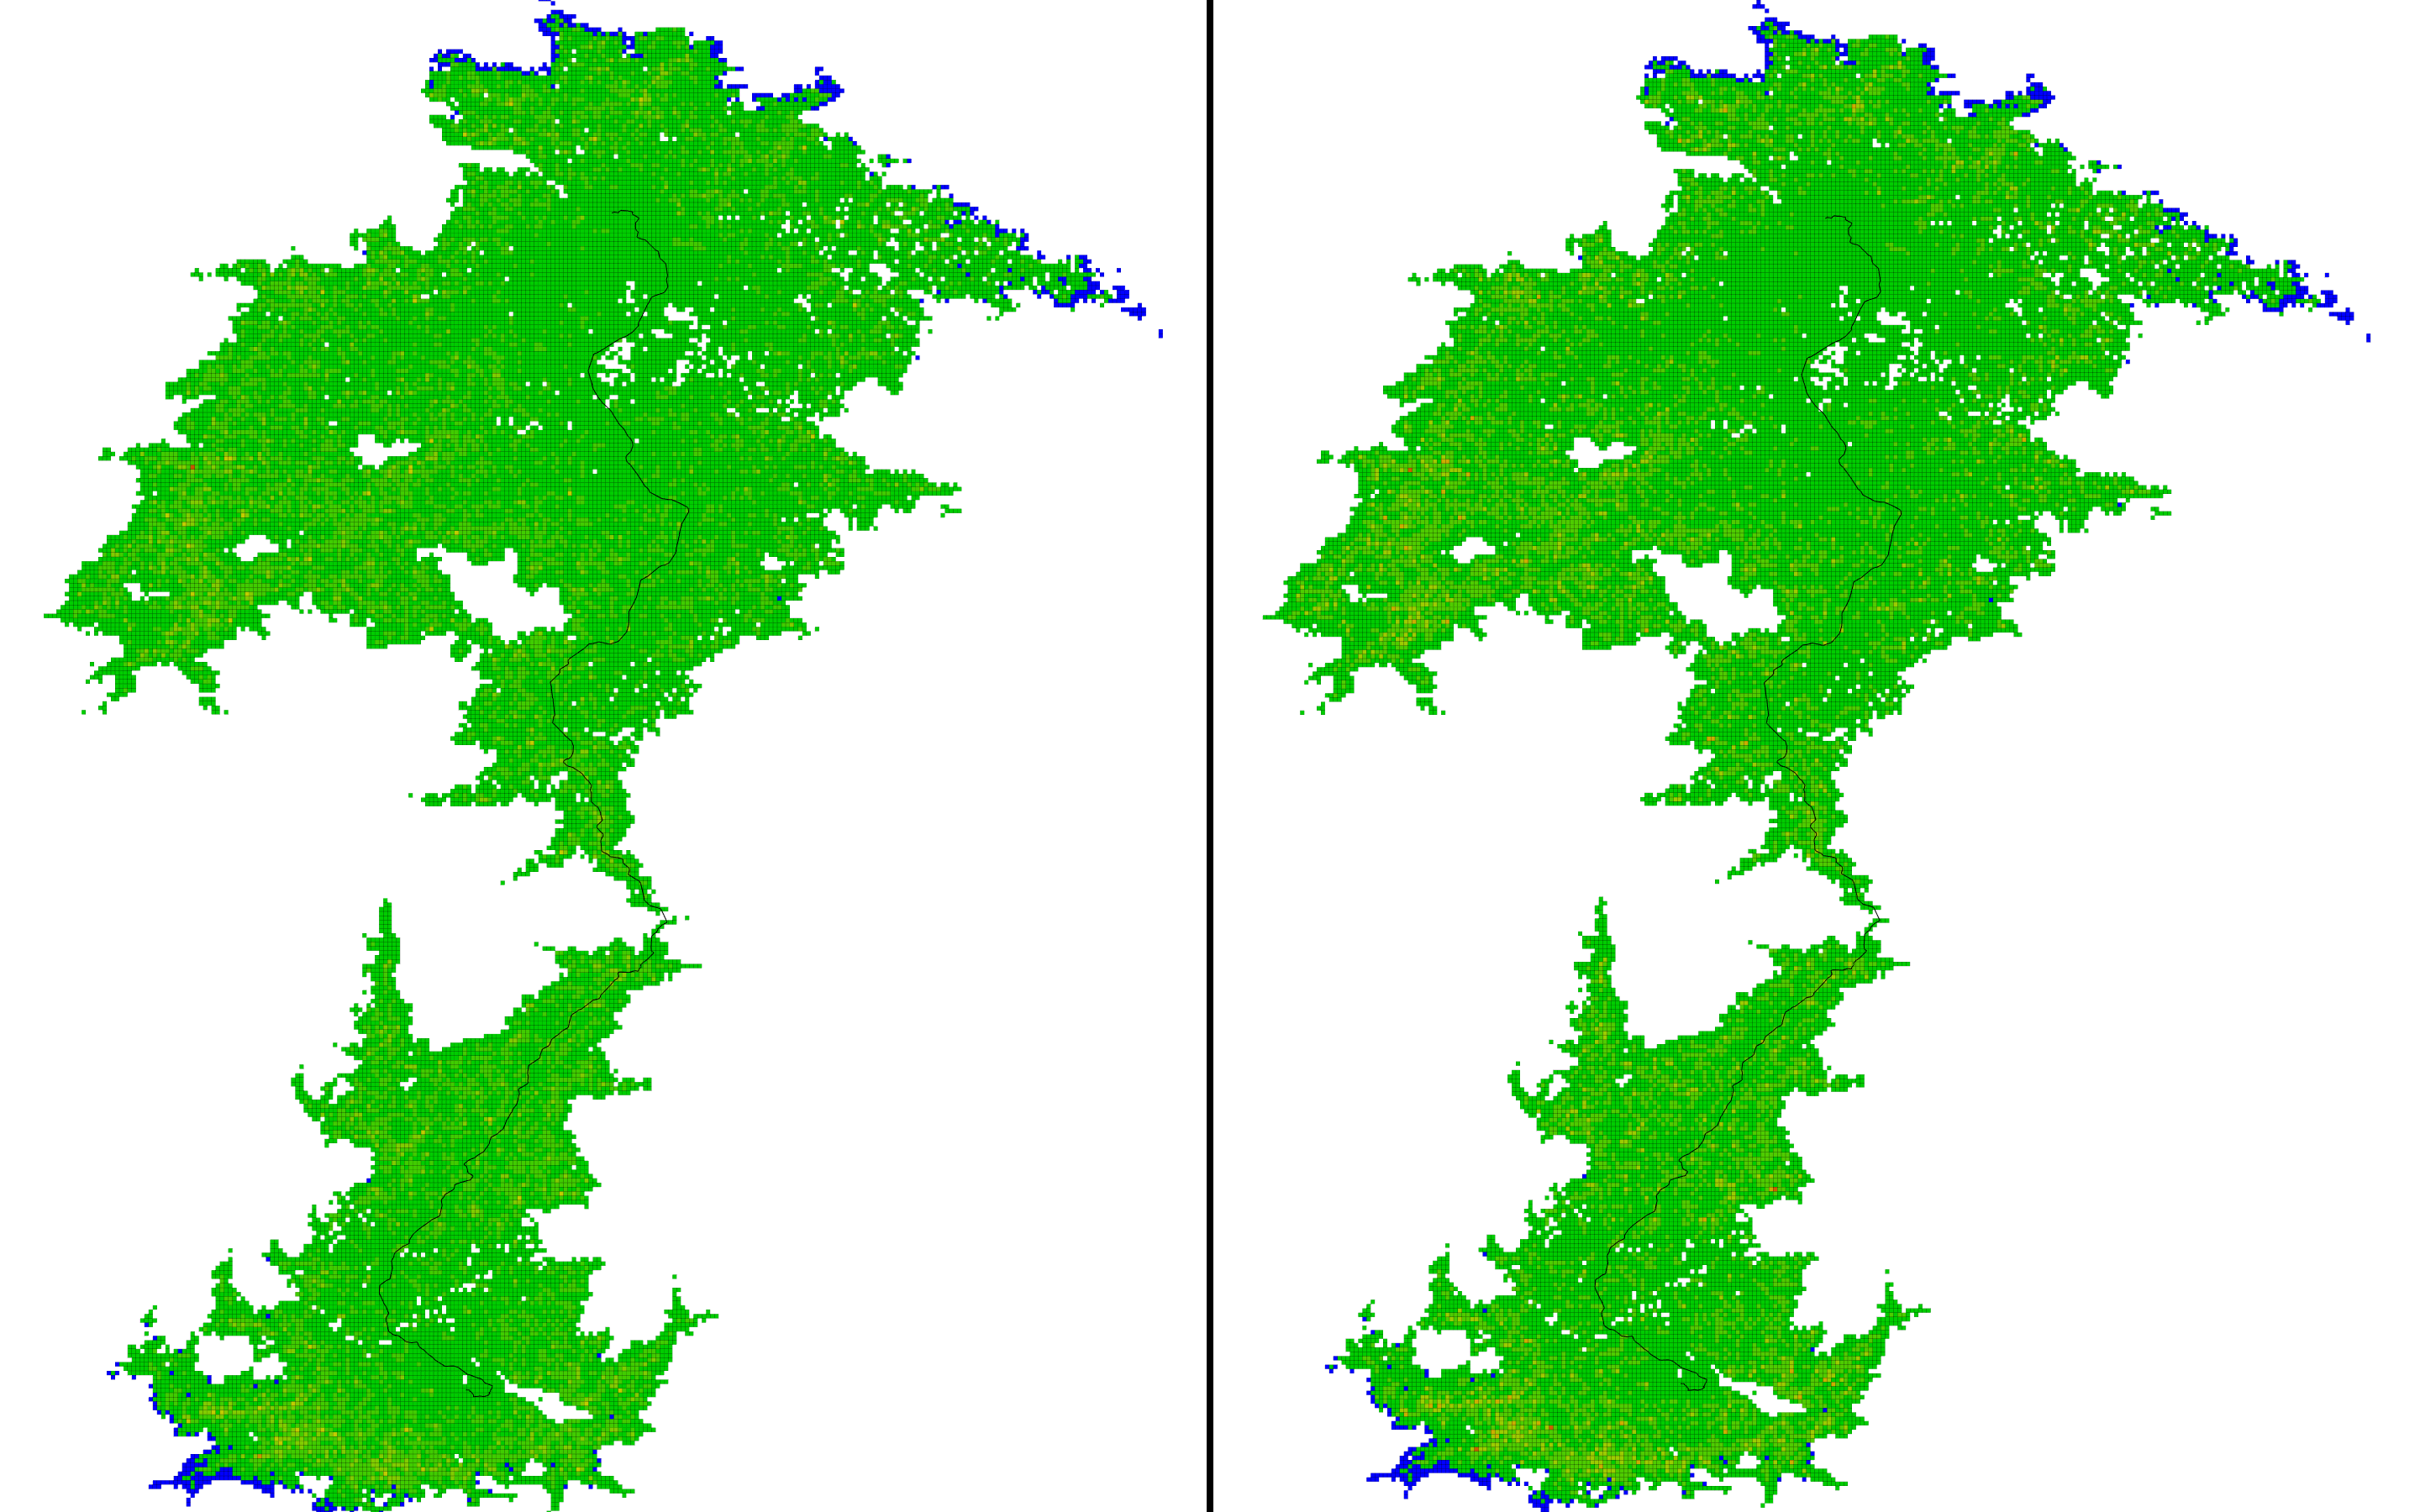
\includegraphics[width=\textwidth]{Images/vis-compare-two.png}
\caption[]{Running two visualizations next to each other.}
\label{fig:two_visualization}
\end{figure}


As a result we can now see rough differences, for example when one algorithm explores more tiles than the other.
Smaller differences, as when some tiles are slightly more loaded than in one of the algorithms are not visible without longer comparison.
That is what we see in \cref{fig:two_visualization}.
The algorithms perform differently, but we can not recognize by just putting both visualizations next to each other.
For comparing algorithms we, therefore, need a new variation of our visualization.
We will now reduce the distance between those two visualizations.
The idea is, that smaller differences are better visible when tiles with the same location are displayed directly next to each other.
Therefore we split each tile in two and color the left half according to the reloads of one algorithm and the right half according to the reloads of the other algorithm.

\begin{figure}[H]
    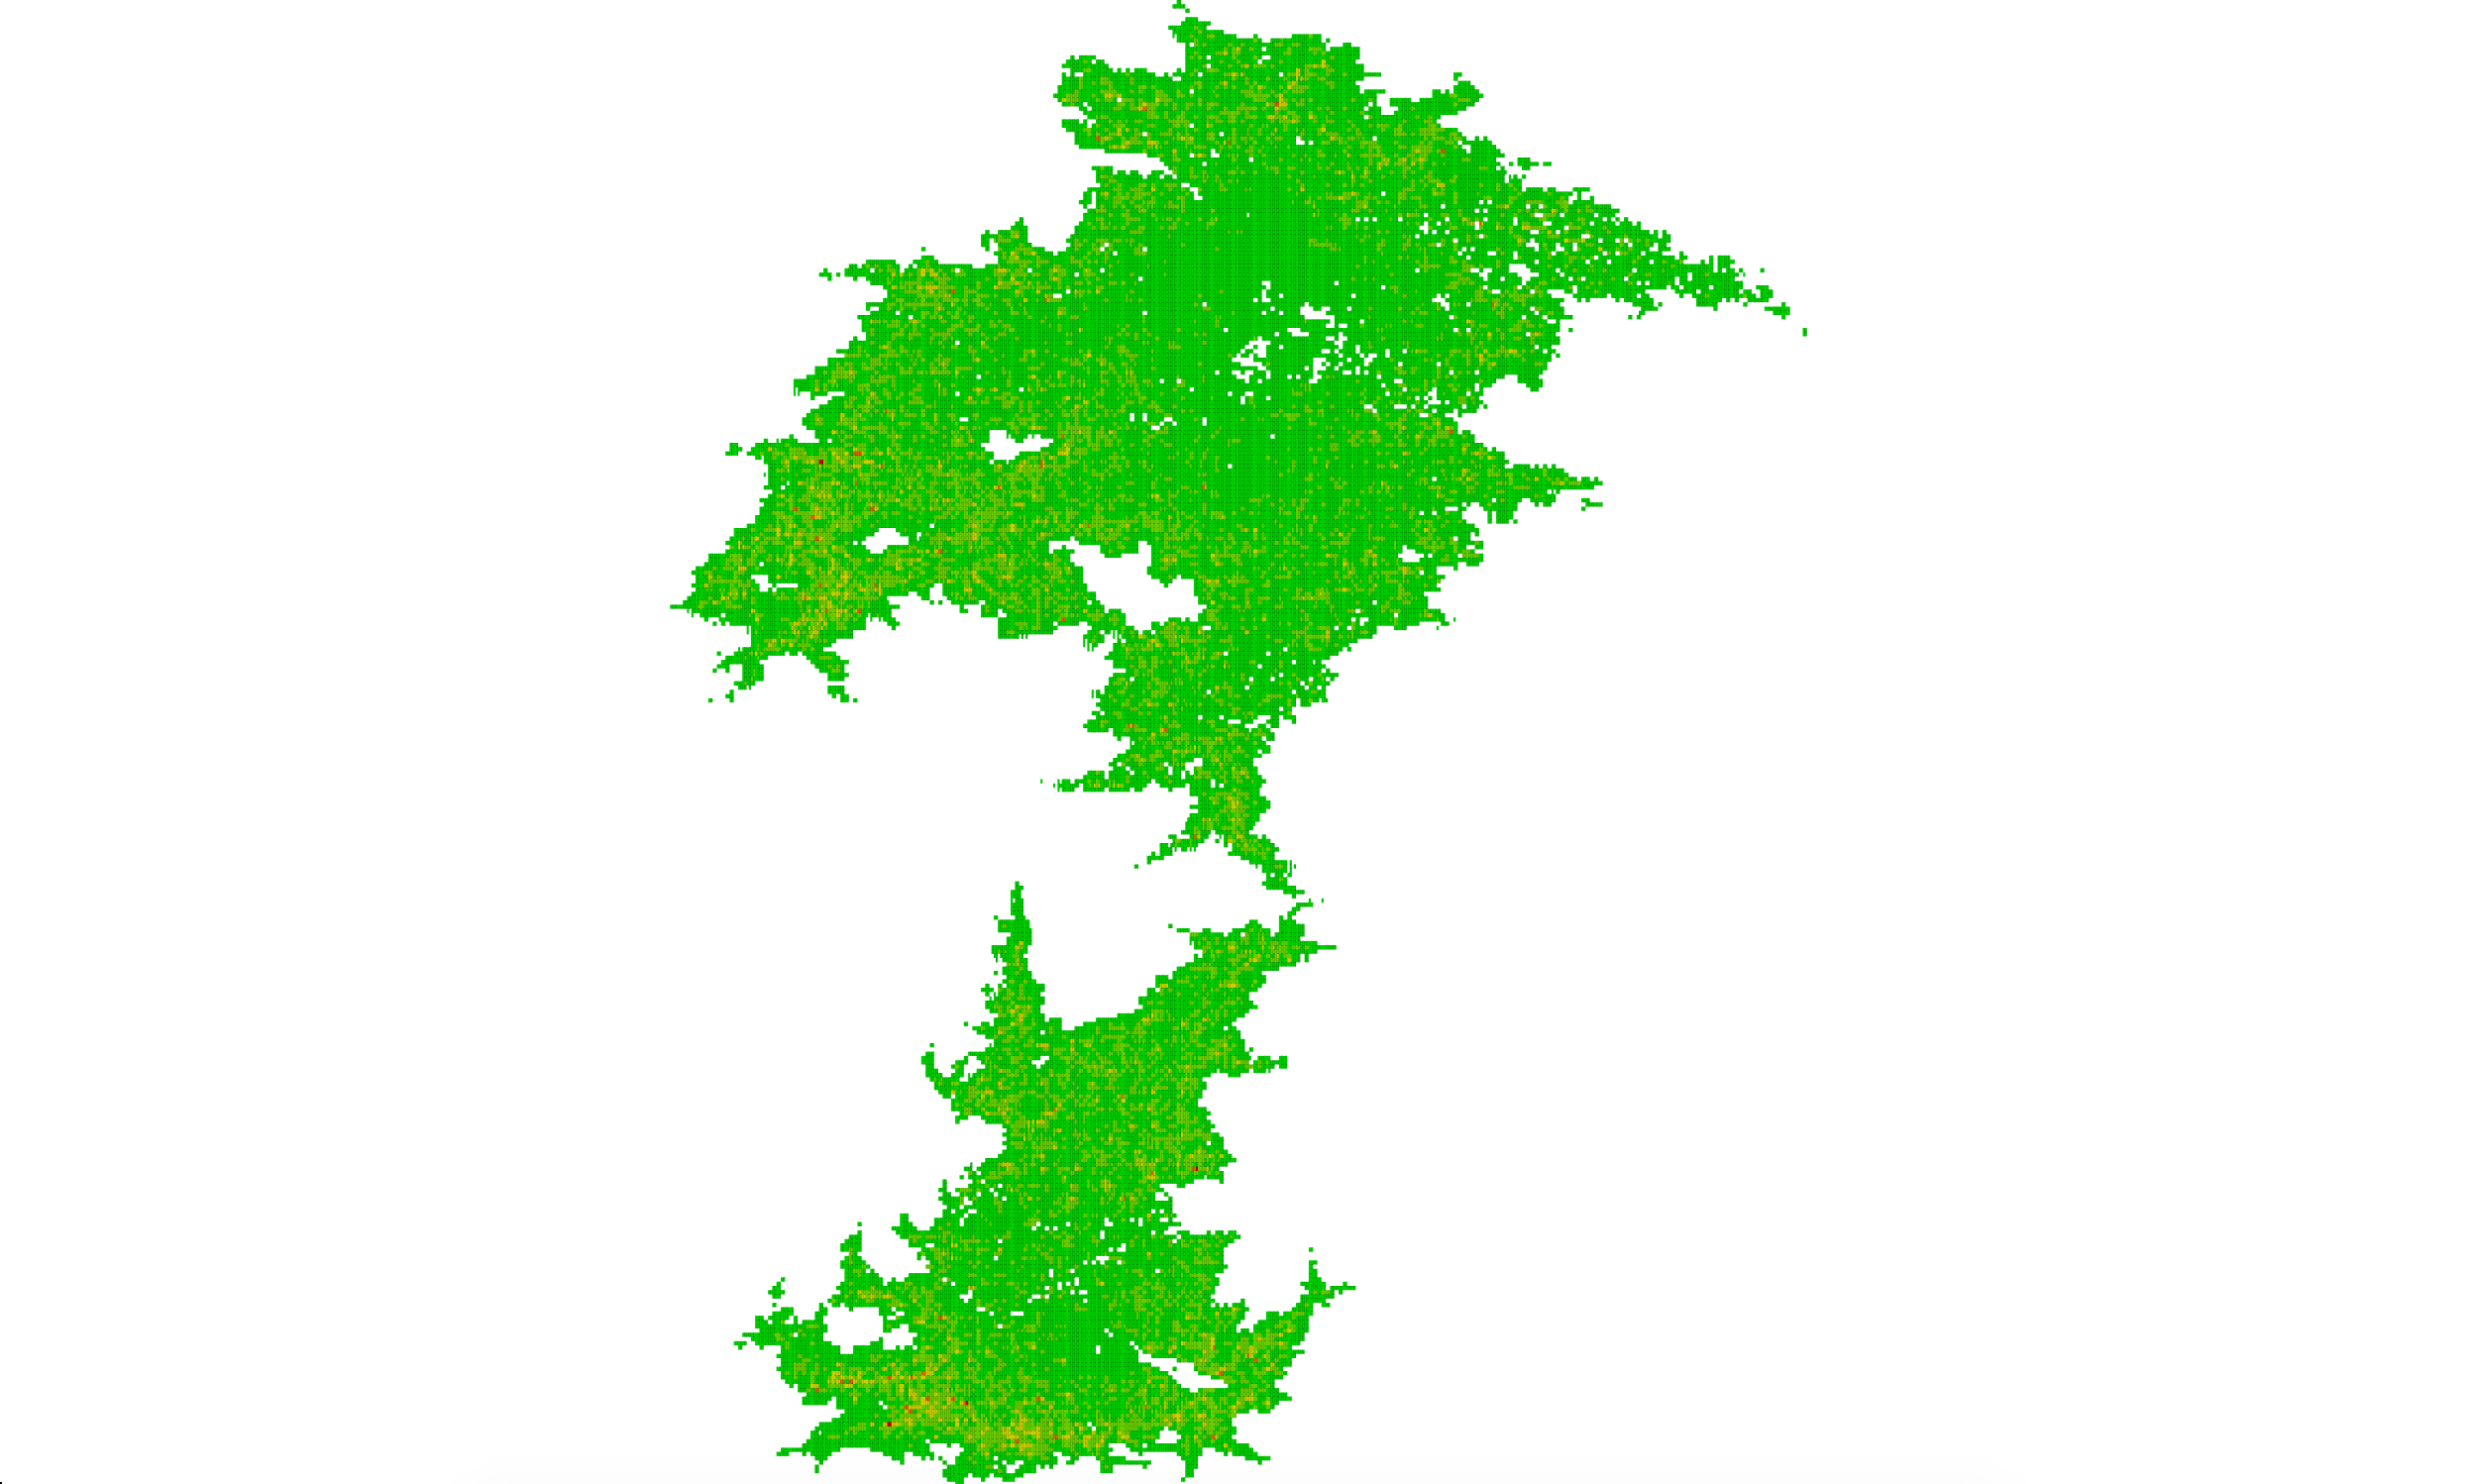
\includegraphics[width=\textwidth]{Images/vis-compare-splitted.png}
\caption[]{Splitting the tiles.}
\label{fig:splitted tiles}
\end{figure}


We now have a much better way to compare two algorithms, as there is no distance anymore between the matching tiles.
However, it is still difficult to clearly identify the differences without longer observation, as the split tiles are quite confusing.
It is very hard to associate one tile with one of the algorithms.
For changing this, we want to think, whether it is necessary to know how often a tile was loaded in a specific algorithm or if showing the difference between the tile loads might lead to a better understanding.\\
Therefore we will try out a different approach as well.
We calculate the difference between the amount of tile loads from both algorithms for each tile.
Then we display all the tiles that have been accessed by at least one algorithm and color those bluish that have been loaded more often by the first algorithm.
Those that have been loaded more often by the second algorithm are colored reddish.
The more intense the color, the bigger is the difference in the amount of tile loads.

\begin{figure}[H]
    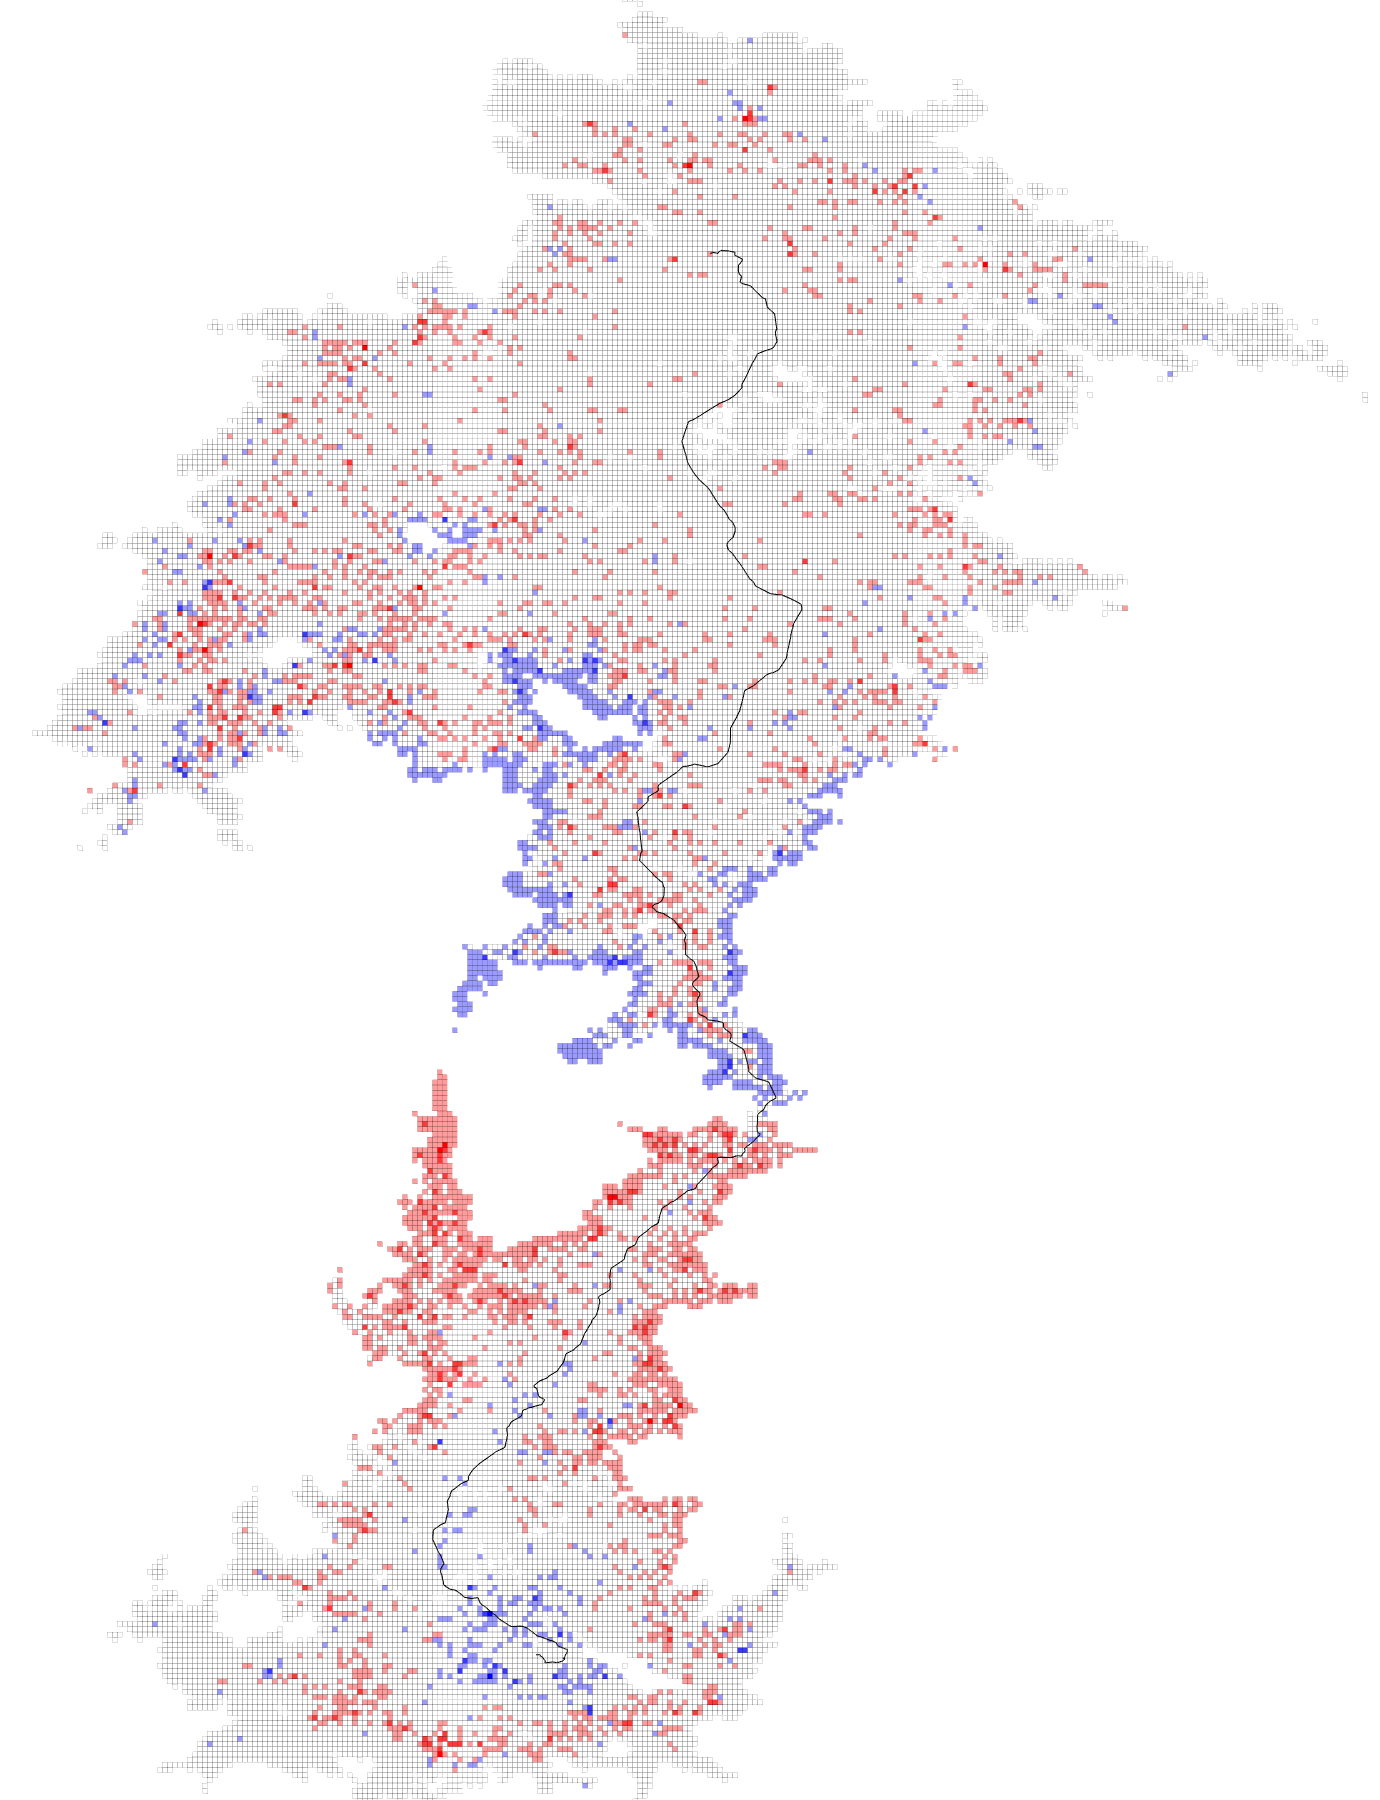
\includegraphics[width=\textwidth]{Images/vis-compare-colored.png}
\caption[]{Showing only the difference of tile loads.}
\label{fig:difference}
\end{figure}

In  \cref{fig:difference} we can now see that both algorithms are similar for most tiles.
Still, there are many tiles that are loaded more often by the second algorithm and even some for which the first algorithm performs better.


\section{Miscellaneous}

In this section, we will take a look on the visualization we have just build and think about some additional features.
For routes with a bigger distance, as for example in \cref{fig:reload_coloring_hsv}, we had to realize, that even the high-level view with displaying only the tiles, the single tiles become quite small.
Therefore we might want to look into the specific region more focussed, which would be possible with a zoom feature.
After having implemented this it is necessary to enable a way to navigate in the graph as well, as otherwise we would be stuck in the middle of the graph.

\begin{figure}[H]
    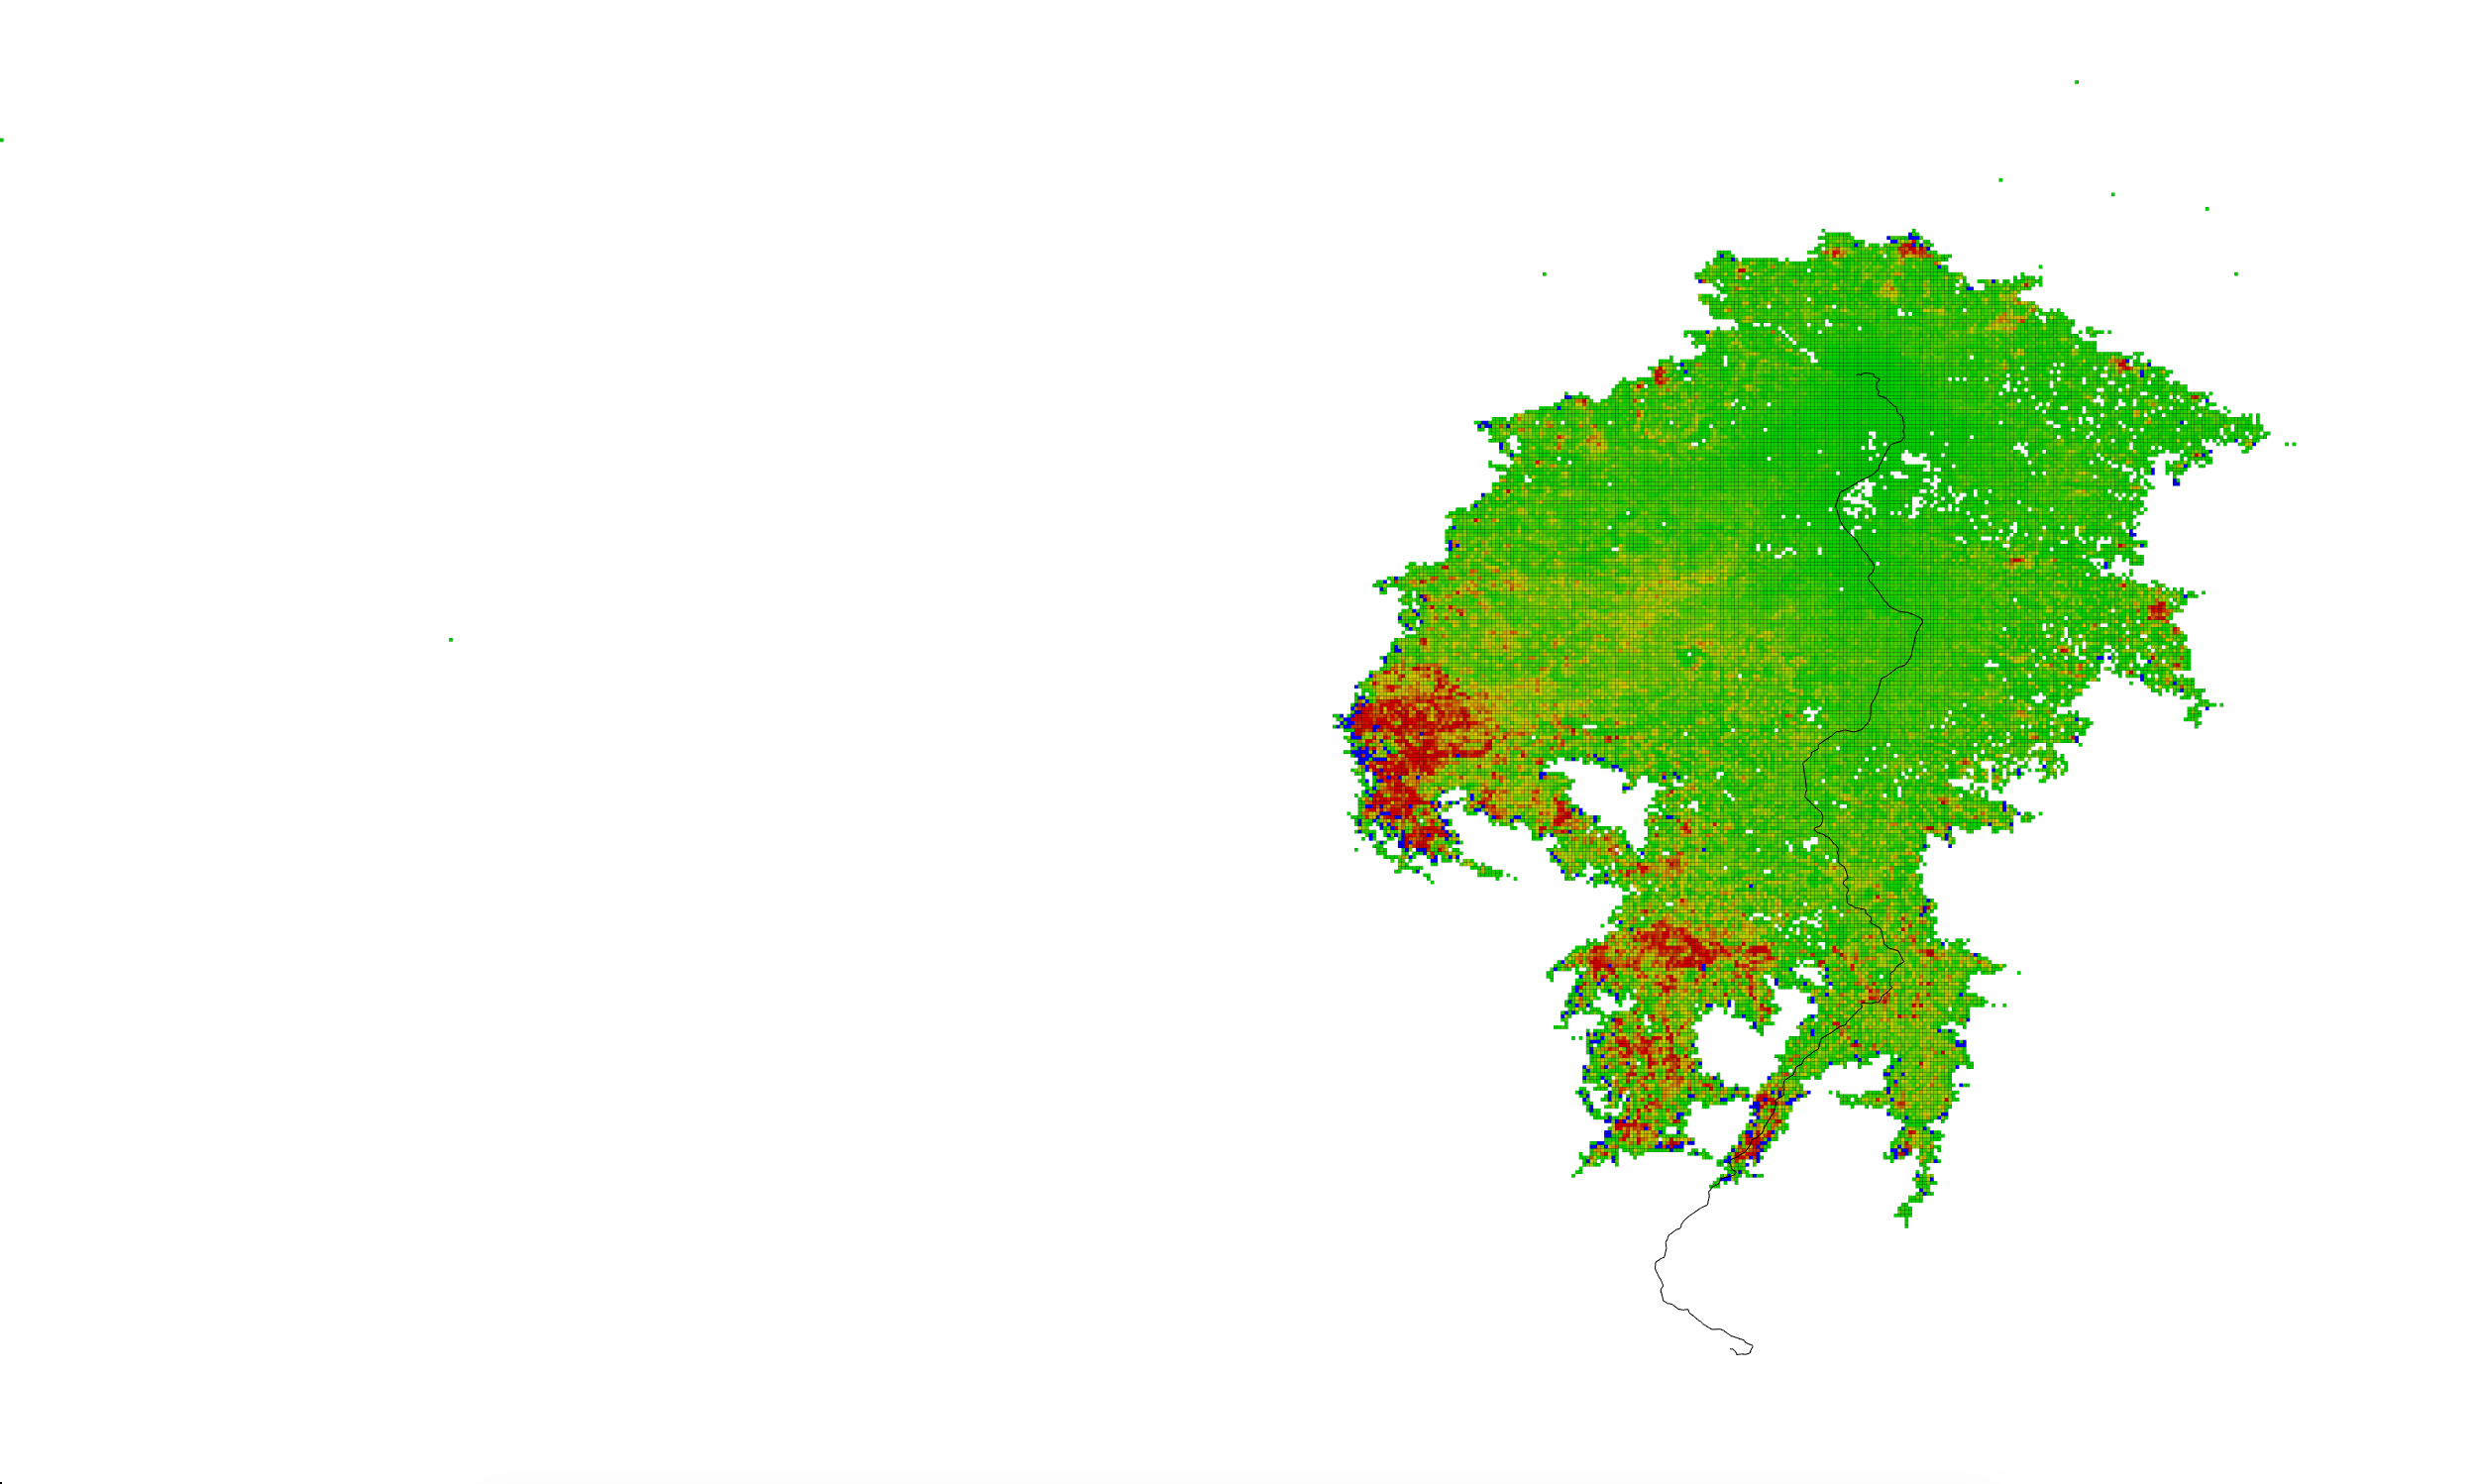
\includegraphics[width=0.5\textwidth]{Images/vis-zoom-small.png}
    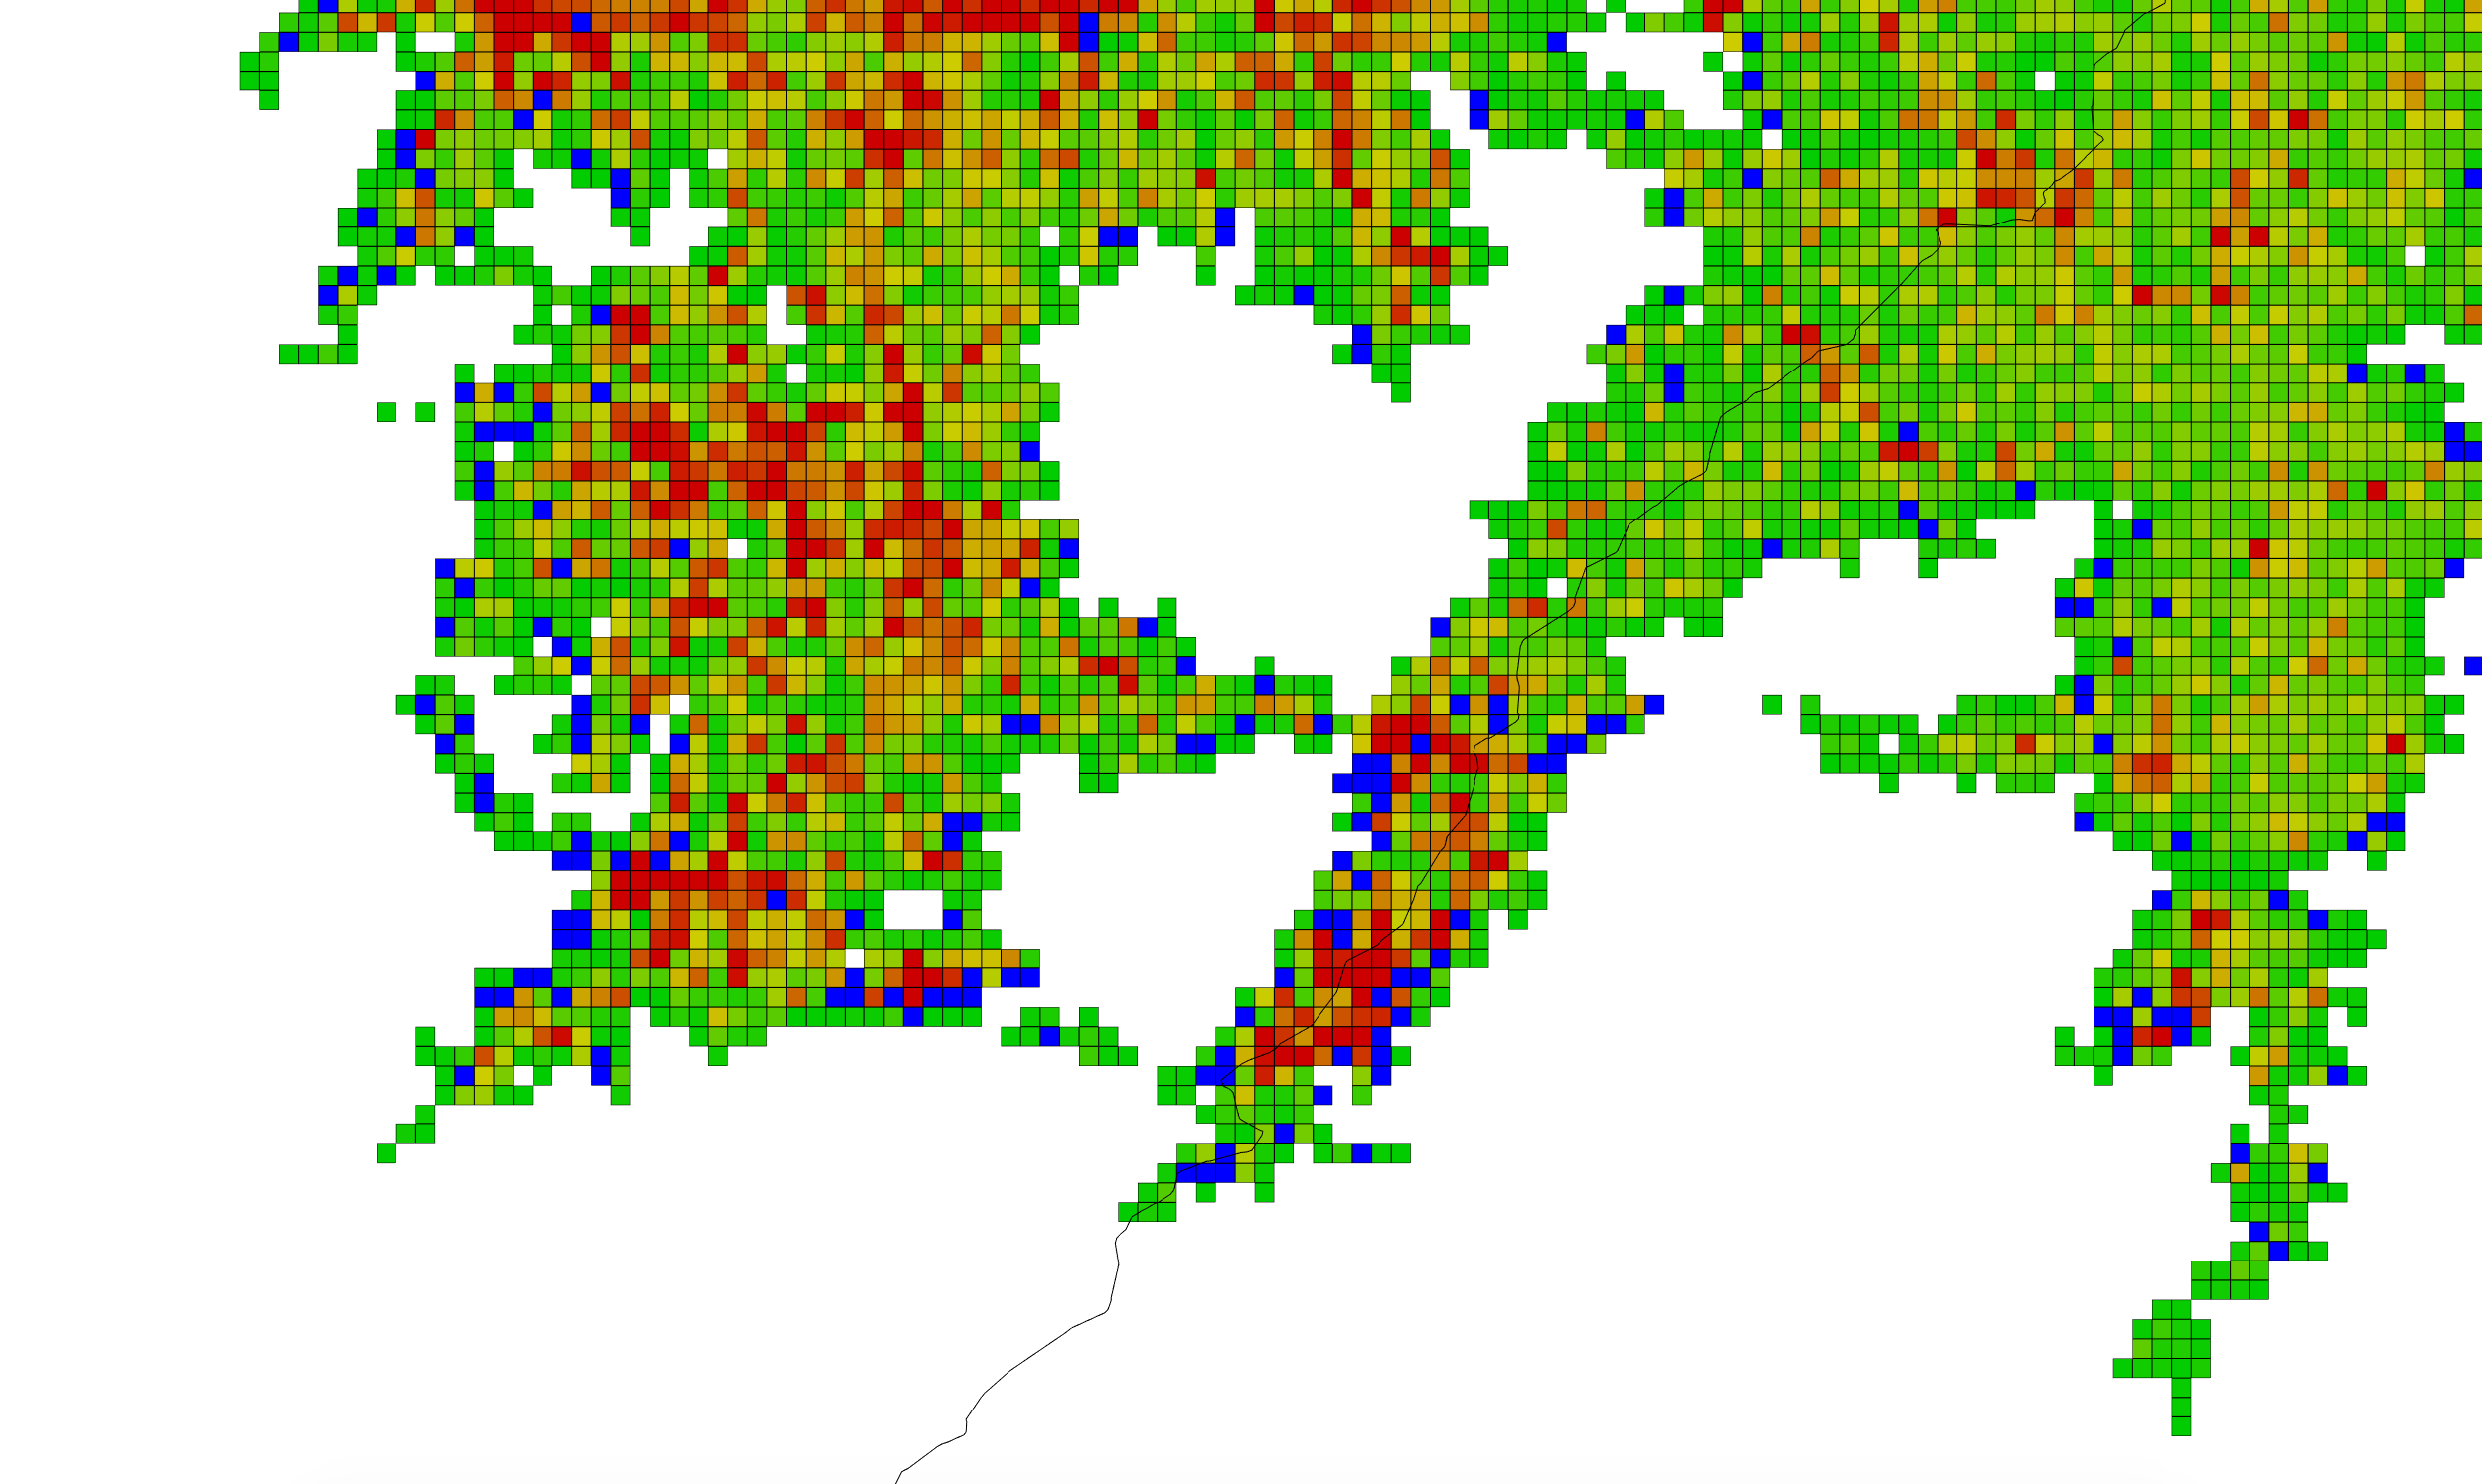
\includegraphics[width=0.5\textwidth]{Images/vis-zoom-large.png}
\caption[]{View on whole graph(left) vz Zoomed view(right)}
\label{fig:zoom}
\end{figure}

We are now able to have a more detailed view on smaller parts of the graph, as we see in \cref{fig:zoom}.\\
In \cref{tiles} we described that the edges are not recognizable individually on bigger routes.
With the possibility of zooming, showing the edges might become a useful feature for our visualization again.
This could, for example, be useful, when we want to understand, why specific tiles are loaded much more than others.
As showing the edges can also make the visualization more confusing and thus distract from the important information, we will make showing the edges optional and make it possible to show and hide them at any point of the visualization.

\begin{figure}[H]
    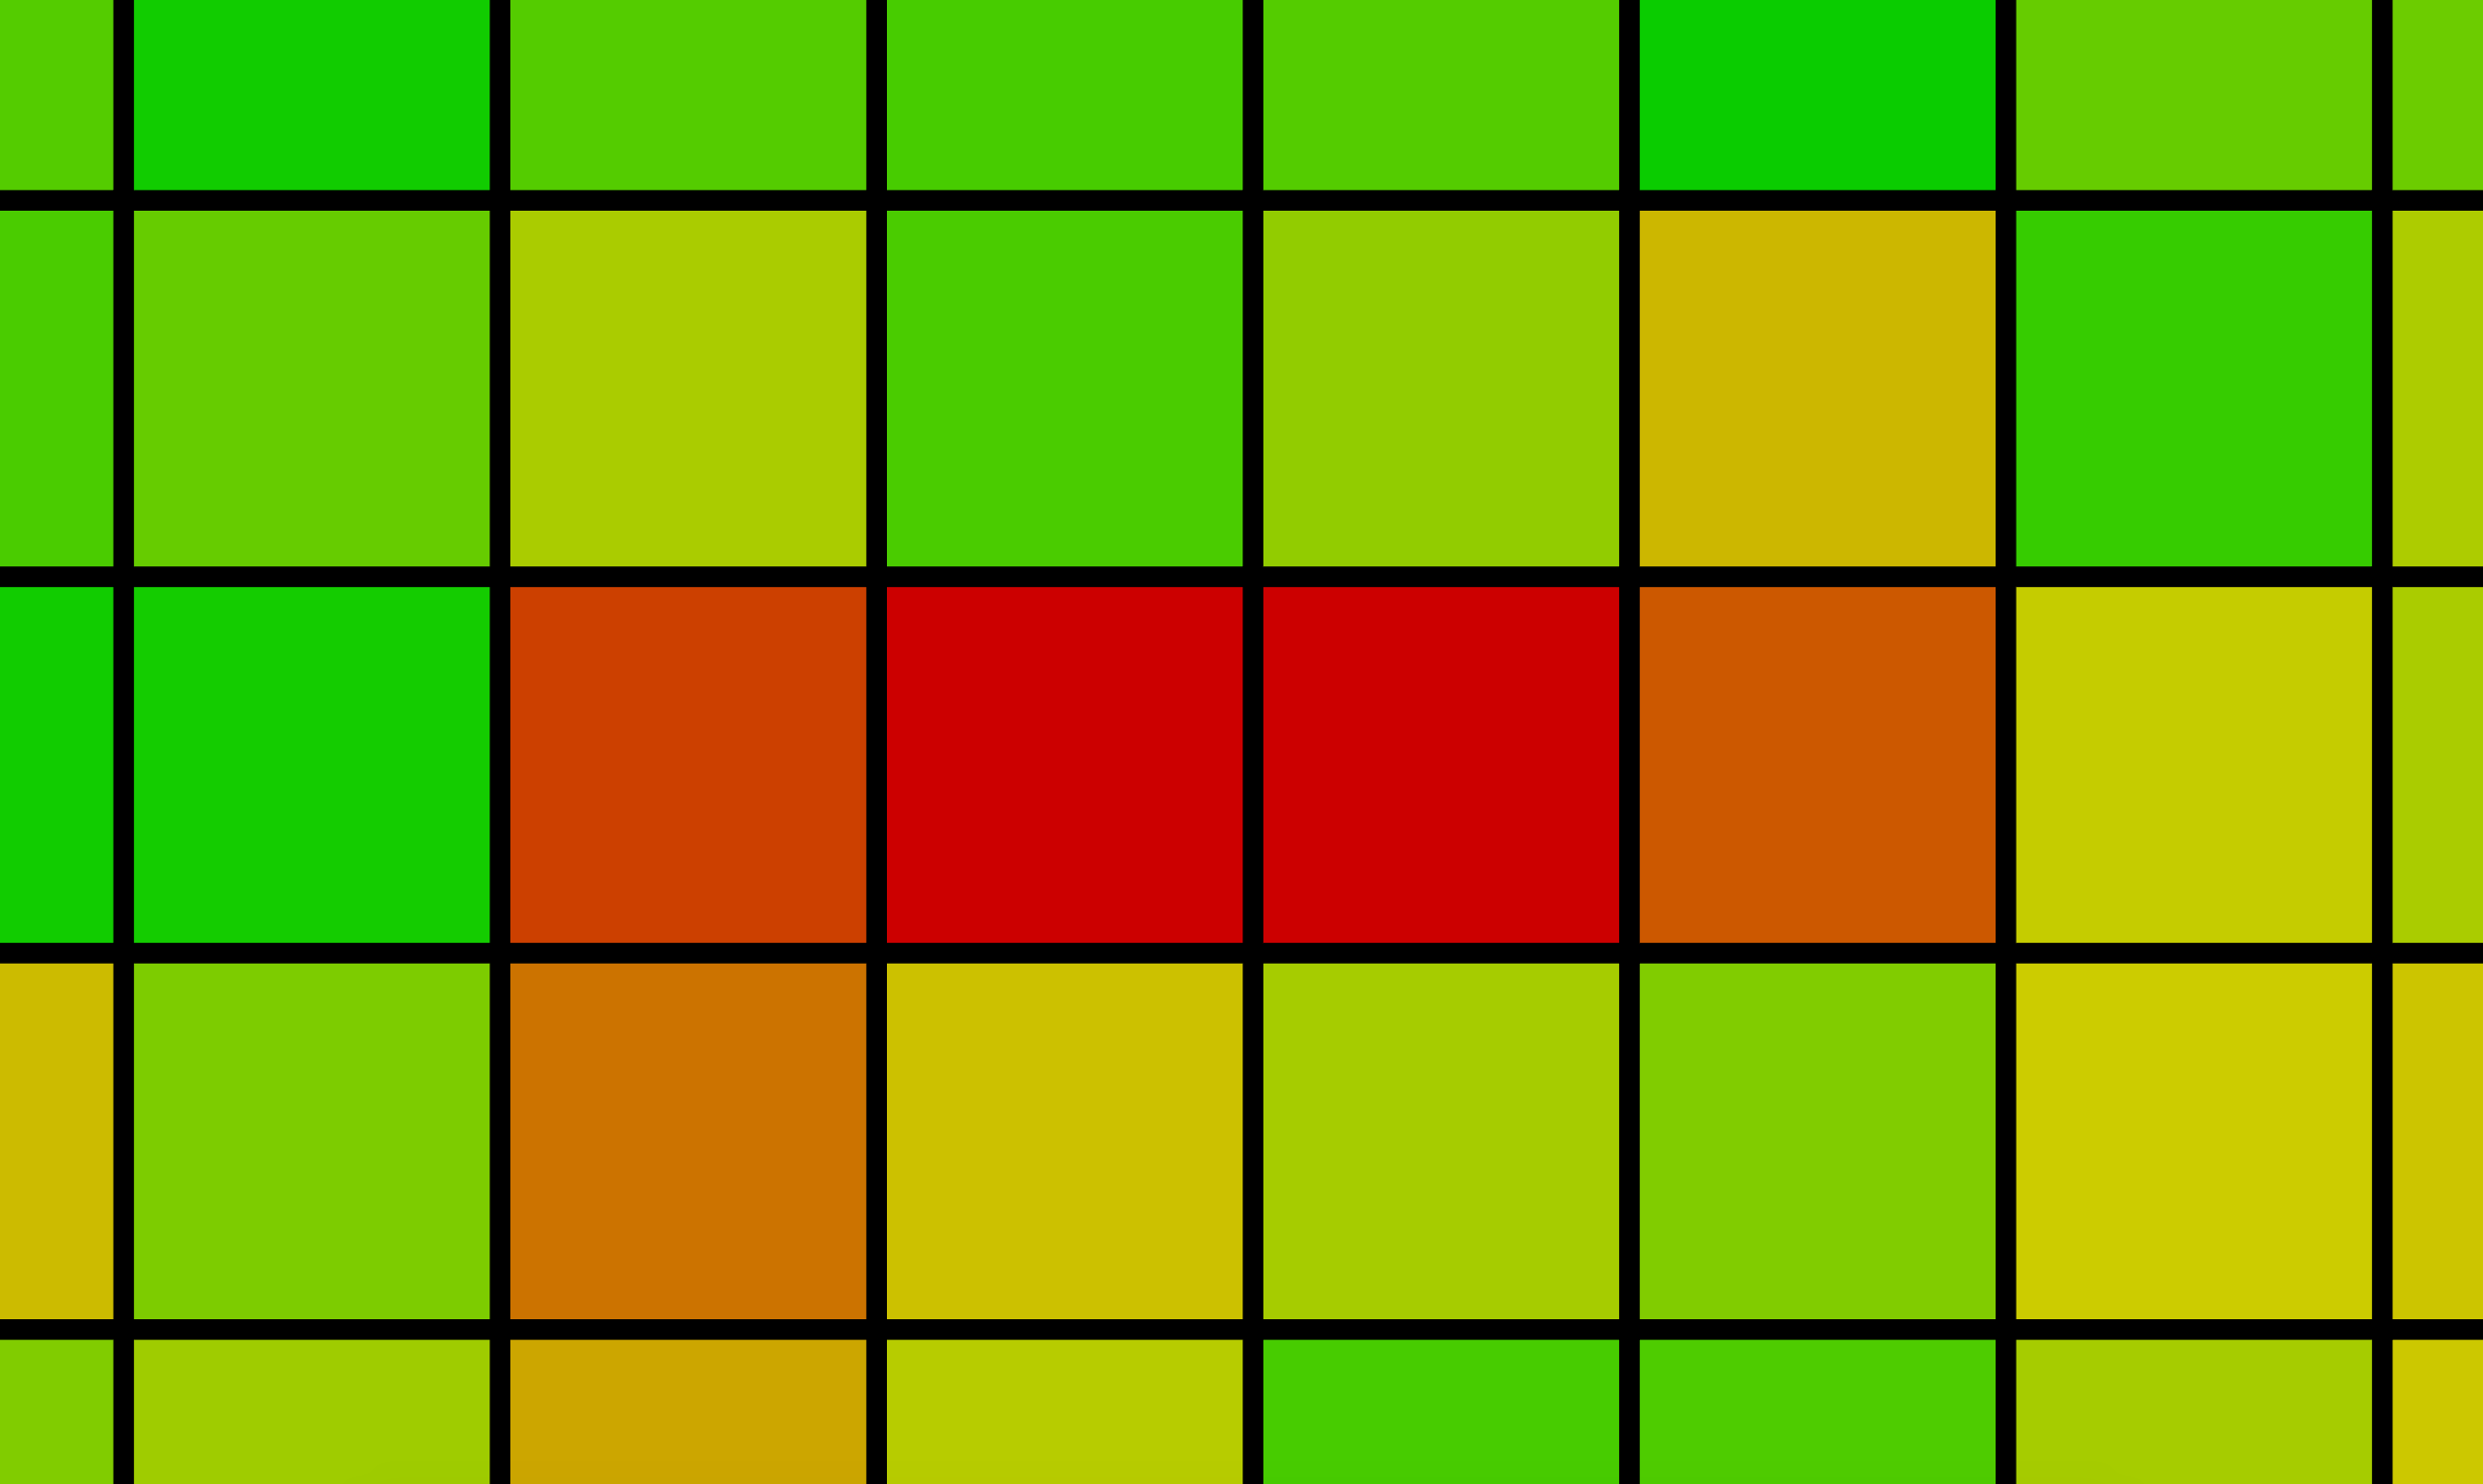
\includegraphics[width=0.5\textwidth]{Images/vis-edges-no.png}
    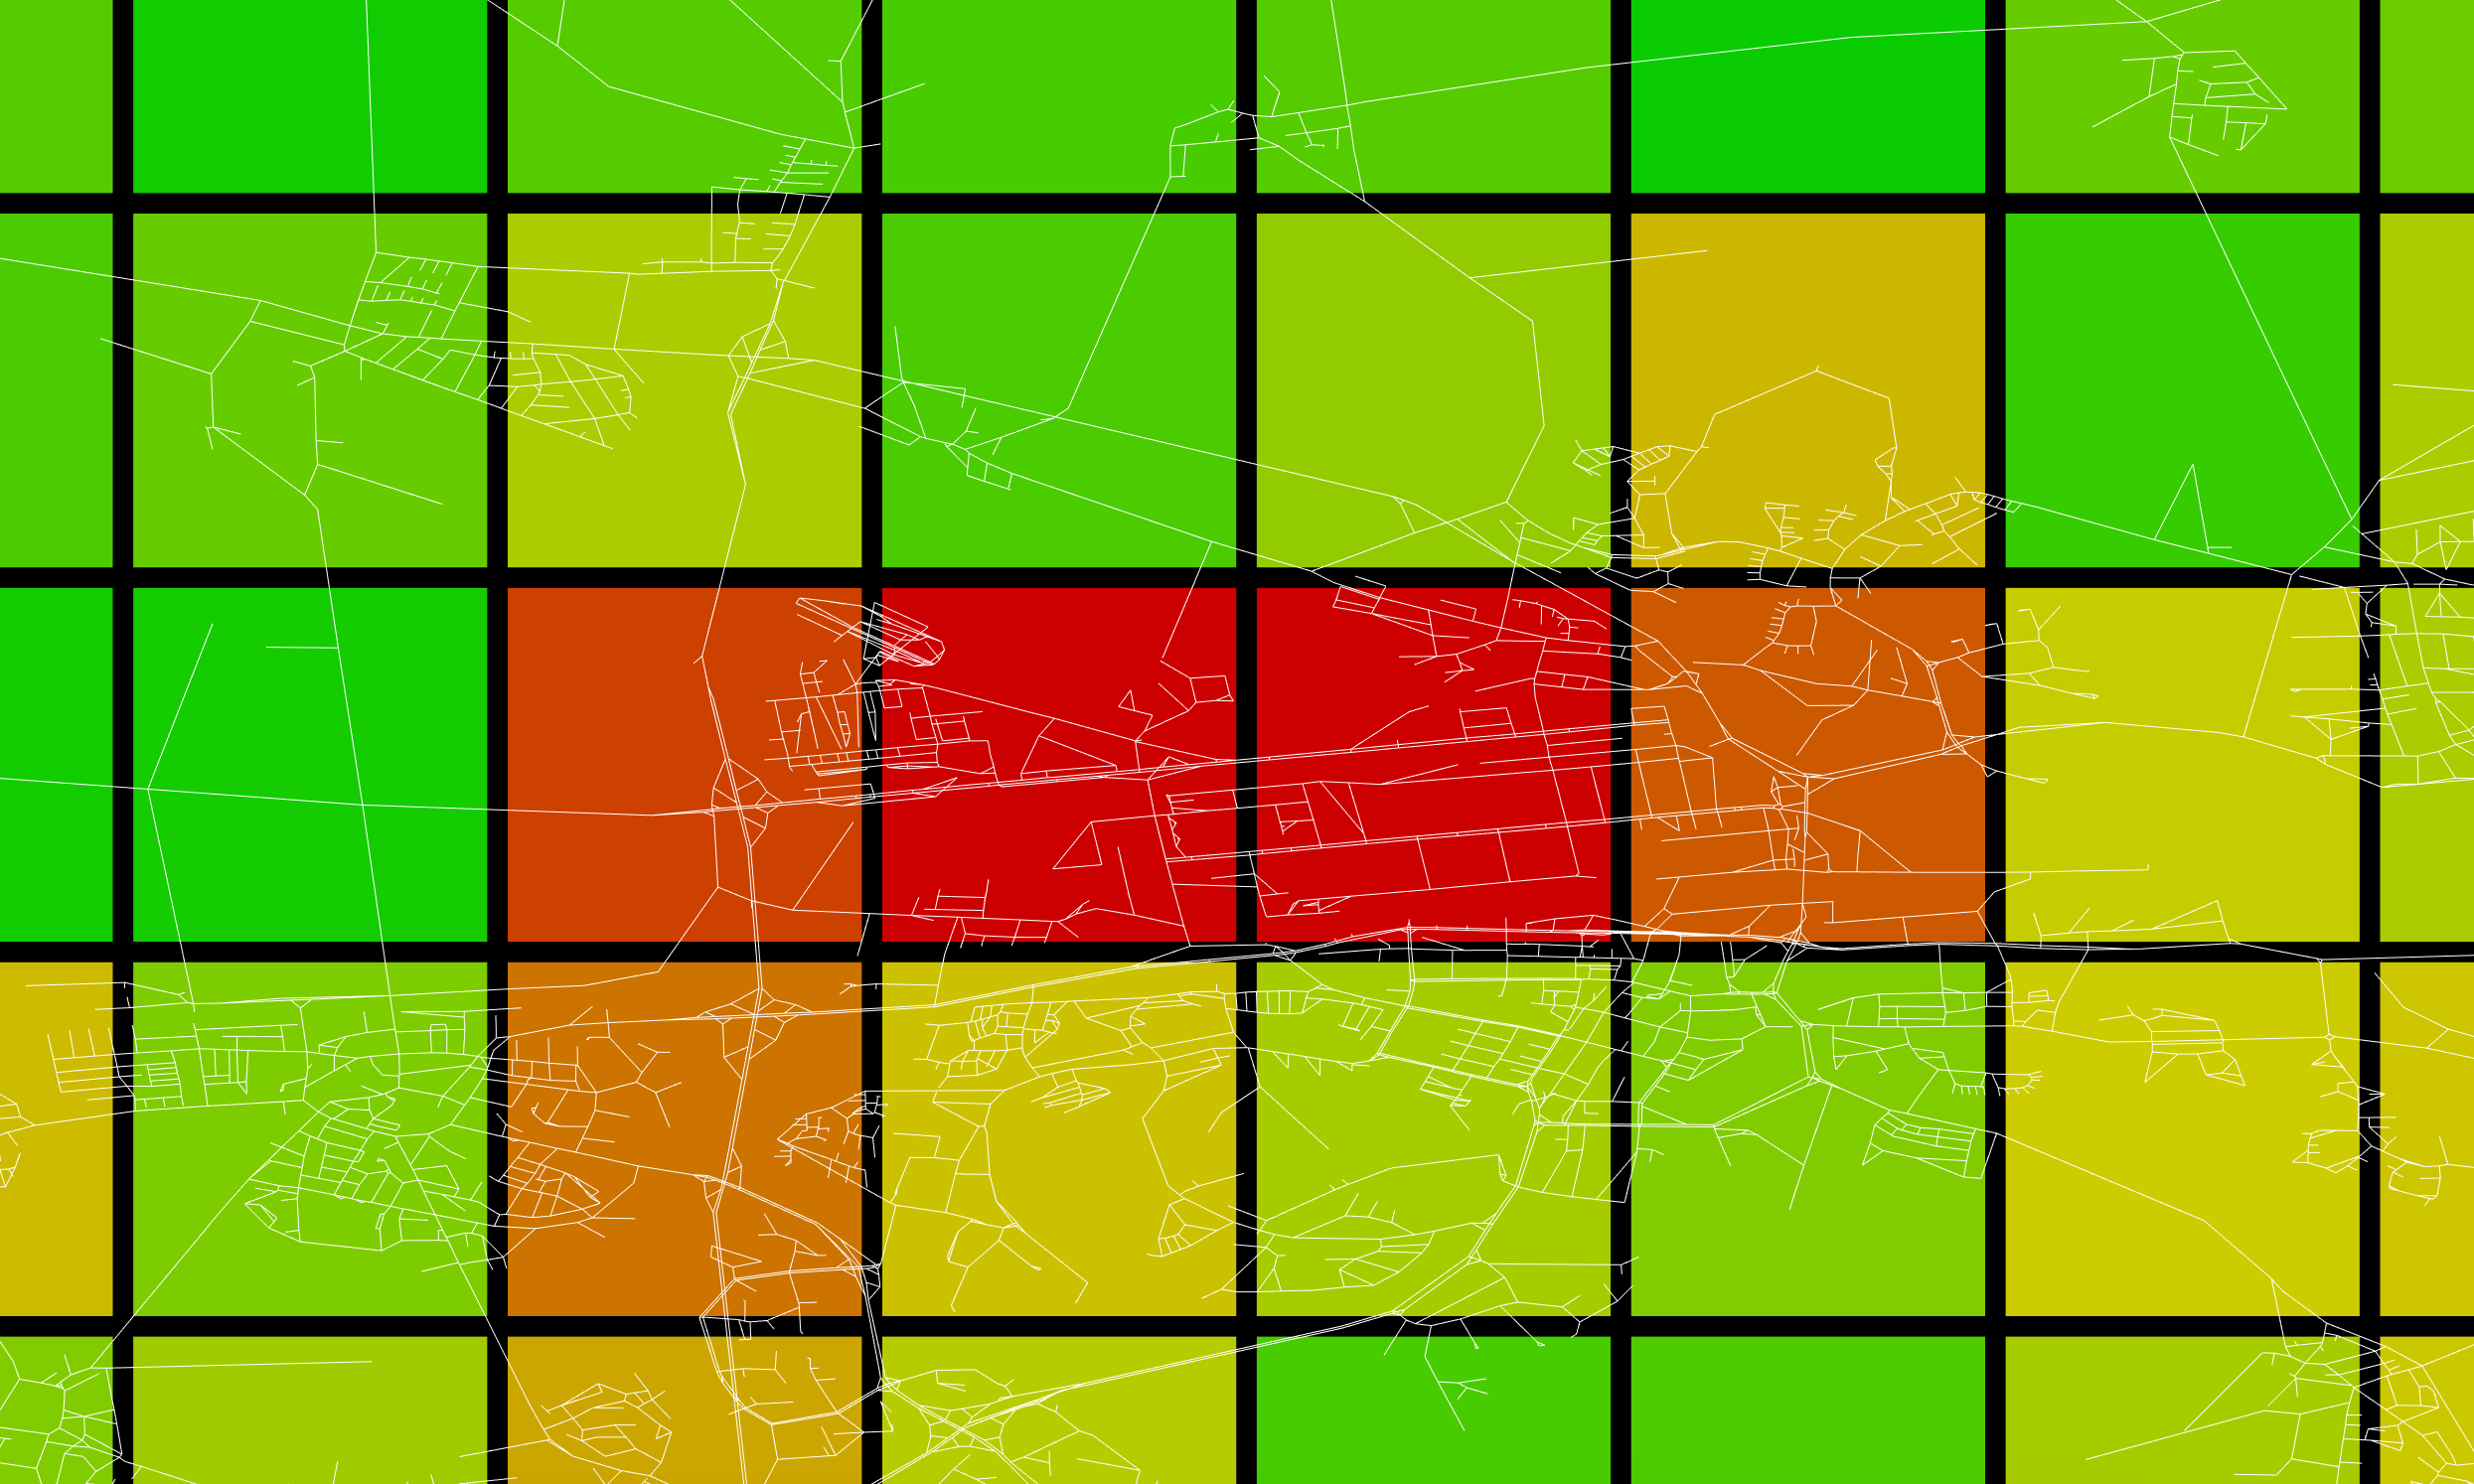
\includegraphics[width=0.5\textwidth]{Images/vis-edges-white.png}
\caption[]{Viewing the graph itself in addition to the tiles.}
\label{fig:white edges}
\end{figure}

Showing the edges helps to understand why some tiles in \cref{fig:white edges} a little in this cases.
The tiles with more reloadings have a high amount of nodes and edges.
Nevertheless, there are also other tiles with many nodes and edges, which are loaded less often.
We will now try to include all additional information we got about the edges into their representation.
As the length of the edges is already represented by the length of the lines in the visualization we only got the speed left to put into the edges.
We will do this by coloring the edges according to their speed.
Starting with red for 0 Km/h and going up to red for up to 150 Km/h.

\begin{figure}[H]
    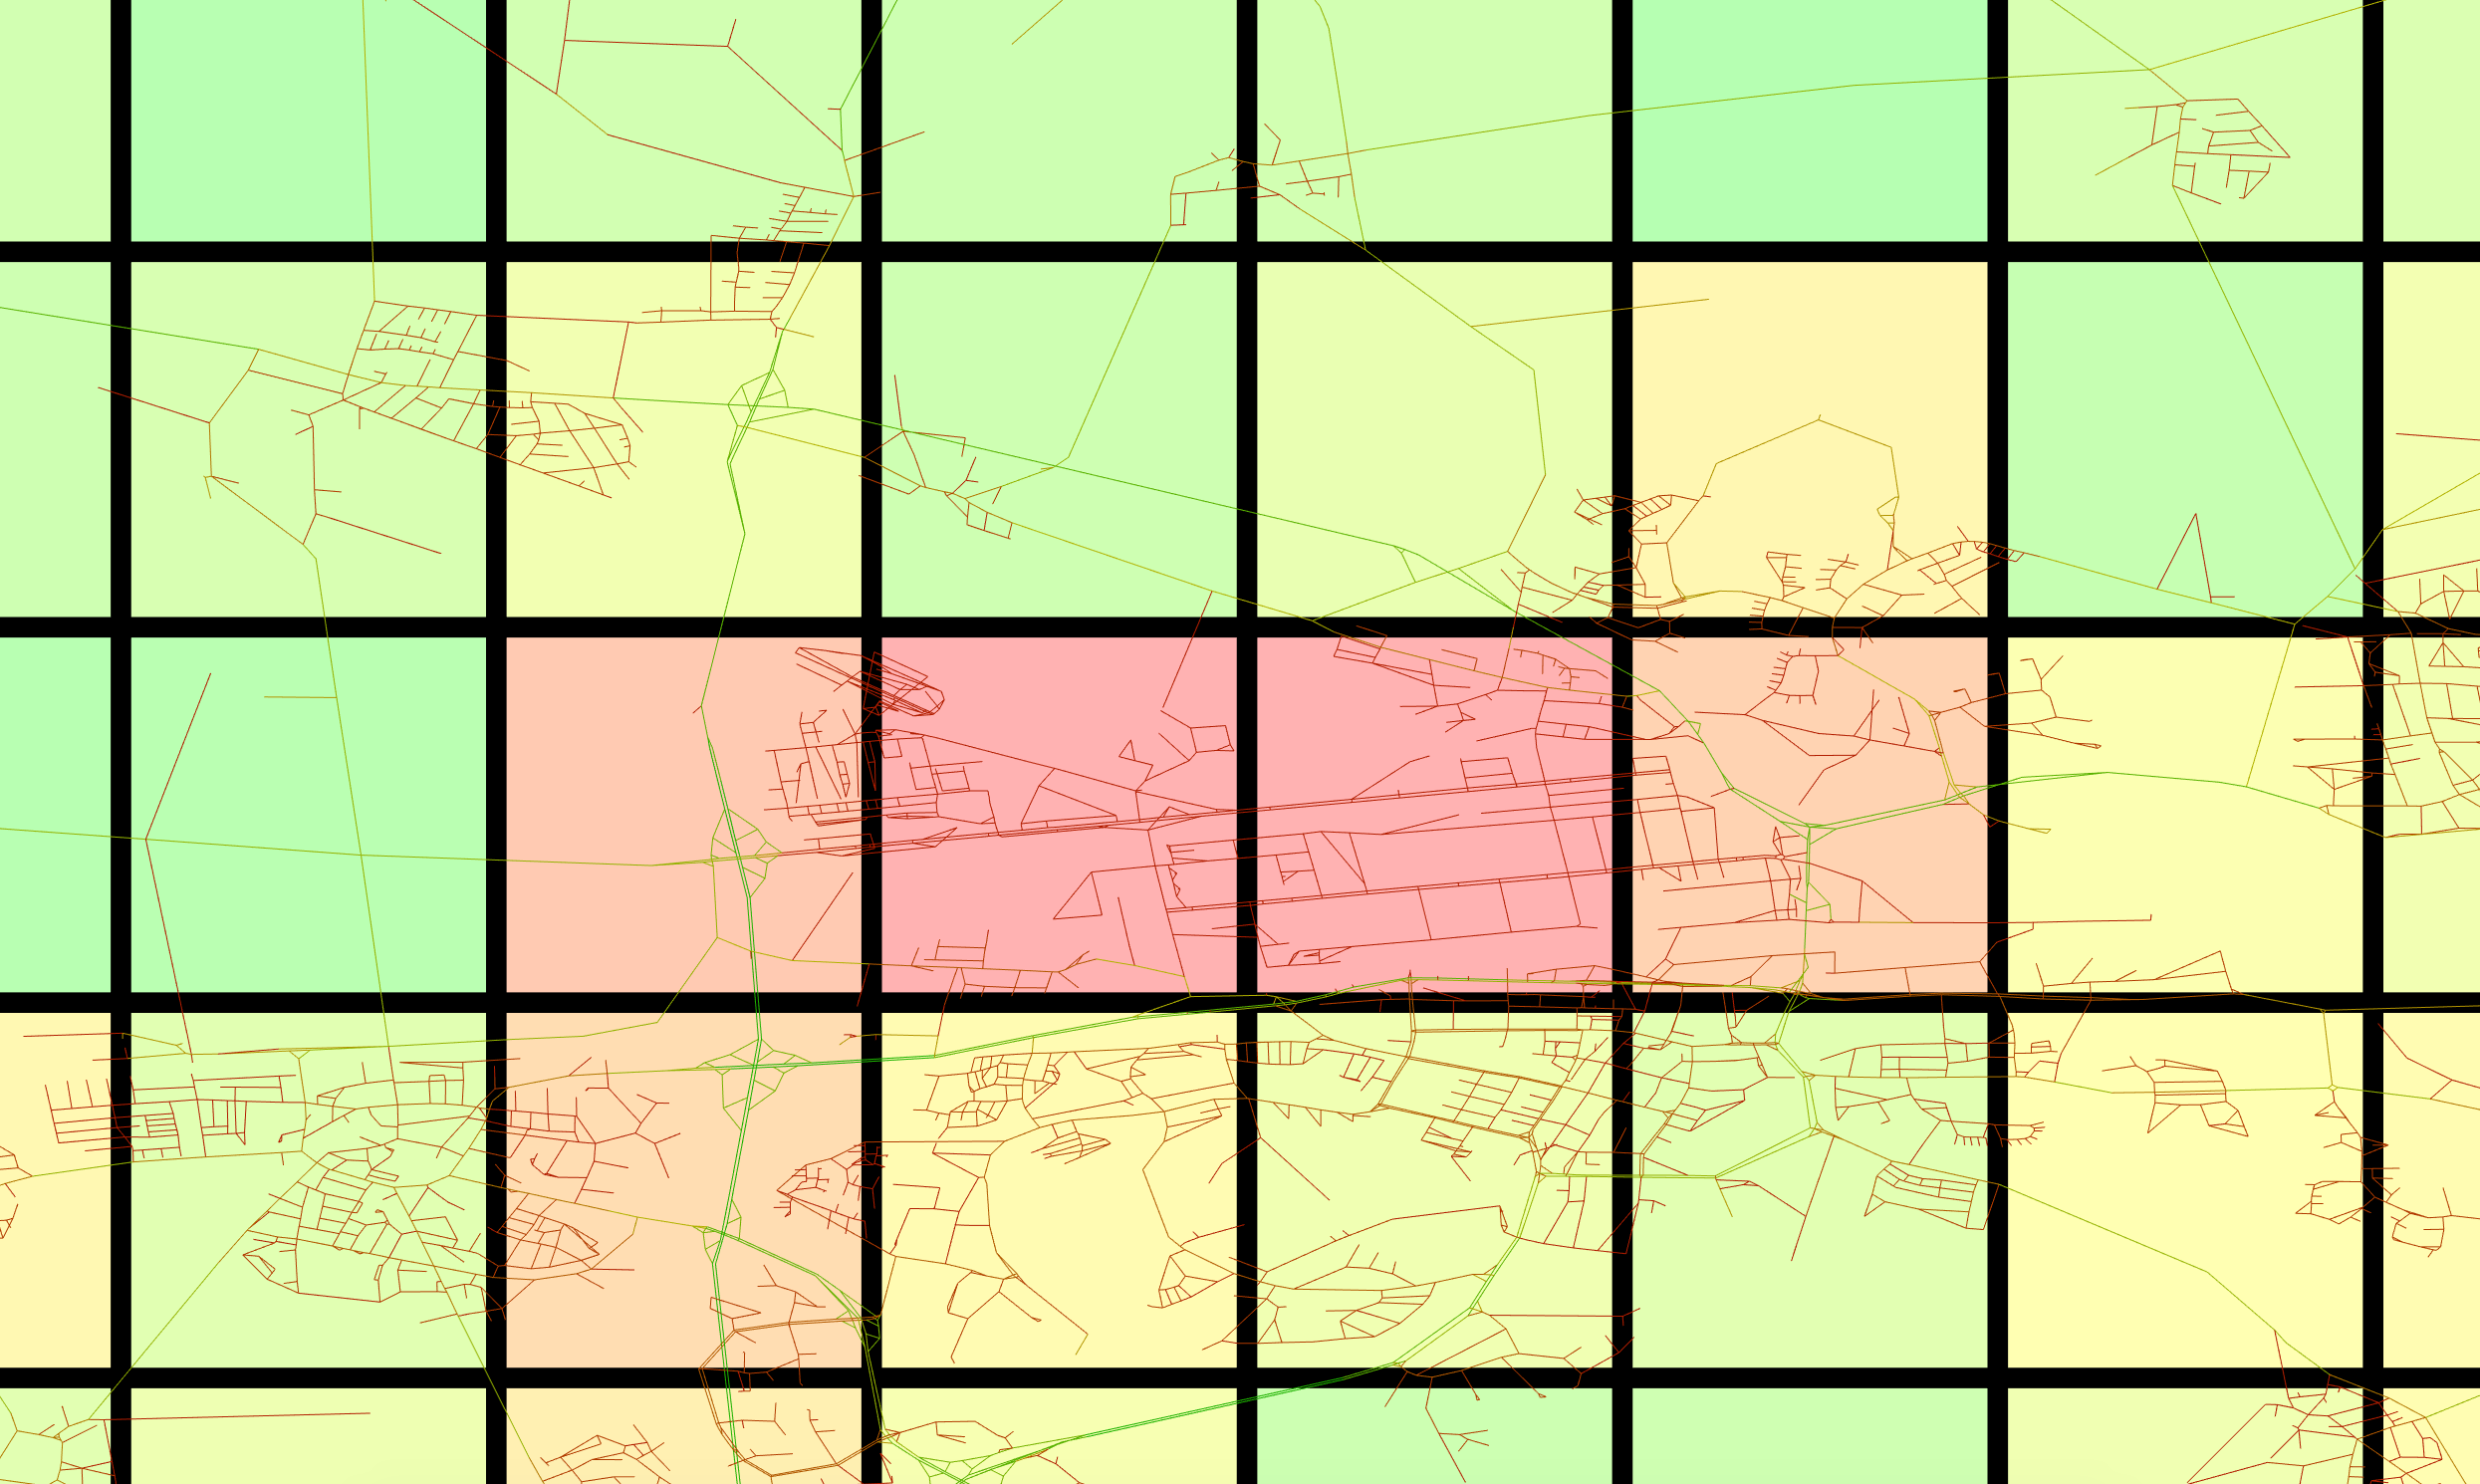
\includegraphics[width=\textwidth]{Images/vis-edges-hsv.png}
\caption[]{Speed based color scheeme. The background had to become a little brighter, when the edges are shown as it would be hard to recognize them clearly. }
\label{fig:colored edges}
\end{figure}

In \cref{fig:colored edges} we can now see that in the tiles that are loaded more often there are not only many edges, but also those with only a small speed.
The surrounding and less loaded tiles allow a higher speed in general.

\chapter{Outlook}
\begin{itemize}
	\item verschiedene Projektionen
	\item knoten anordnen mit kanten mit länge = kosten
	\item different layers
	\item gerichtete edges
\end{itemize}

% References
\renewcommand*{\bibname}{References}
\bibliographystyle{abbrvnat}
\bibliography{Files/References}


\chapter*{Independence Declaration}
\addcontentsline{toc}{chapter}{Declaration of Authorship}
\thispagestyle{empty}

I hereby declare that the thesis submitted is my own unaided work. All direct or indirect sources used are acknowledged as references.\vspace{2 ex}

Potsdam, \today\\[6 ex]

\begin{flushleft}
    \begin{tabular}{p{5cm}}
        \hline
        \centering\footnotesize\printAuthor
    \end{tabular}
\end{flushleft}


\end{document}
